\documentclass{xdupgthesis}

% XDUTS核心配置
\xdusetup{
  style = {
    customize-los = false,
    customize-loa = false,
    % 关闭DOI和URL链接
    biblatex-option = {doi=false, url=false},
  },
  info = {
    graduate-type         = 硕士,
    degree-type           = 学术,
    % 核心必填信息
    title                 = {面向双车道高速公路的多地磁传感器车辆目标跟踪方法研究},
    title*                = {Research on Vehicle Target Tracking Methods Using Multiple Geomagnetic Sensors for Two-Lane Expressways},
    author                = {侯照莹},
    author*               = {Zhaoying Hou},
    department            = {通信工程学院},
    major                 = {信息与通信工程},
    major*                = {Information and Communication Engineering},
    sub-major             = {通信计算融合与场景应用},
    student-id            = {23011210459},
    supervisor            = {毛国强},
    supervisor*           = {Guoqiang Mao},
    supv-title            = {教授},
    supv-title*           = {Professor},
    supervisor-enterprise = {},
    supervisor-enterprise*= {},
    supv-ent              = {},
    supv-ent*             = {},
    supv-ent-title        = {},
    supv-ent-title*       = {},
    supervisor-title      = {教授},
    supervisor-title*     = {Professor},
    supervisor-enterprise-title  = {},
    supervisor-enterprise-title* = {},
    %%自己新增申请学位类别
    degree = {工学硕士},
    % 学科与保密信息
    domain                = {新一代电子信息技术（含量子技术等）},
    clc                   = {TP391.41},
    secret-level          = {公开},
    submit-date           = {2026-04-01},
    % 关键词
    keywords              = {车辆目标跟踪，地磁传感器，卡尔曼滤波，数据关联，在线聚类},
    keywords*             = {Vehicle Target Tracking, Geomagnetic Sensor, Kalman Filtering, Data Association, Online Clustering},
    % 附件与声明文件
    abstract              = {chapters/abstract-zh.tex},
    abstract*             = {chapters/abstract-en.tex},
    acknowledgements      = {chapters/acknowledgements.tex},
    bio                   = {chapters/biography.tex},
    appendix              = {chapters/appendix1.tex},
    statement-scan        = {},
    statement-sign        = {},
    los                   = {chapters/los.tex},
    loa                   = {chapters/loa.tex},
    % 参考文献
    bib-resource          = {references.bib},
  }
}

% -------------------------
% 常用包（按功能分组）
% -------------------------
\usepackage{graphicx}
\graphicspath{{images/}}

\usepackage{amsmath}
\usepackage{amsfonts}
\usepackage{amssymb}

\usepackage{booktabs}
\usepackage{multirow}
\usepackage{makecell}
\usepackage{tabularx}
\usepackage{threeparttable}

\usepackage{subcaption}

\usepackage{xcolor}
\usepackage{pifont}

\usepackage{enumitem}


\usepackage{graphicx}
\graphicspath{{E:/MyLunWen/xduts-main/code/chapter4/experiment123/result/}}
 \usepackage{booktabs}
 \usepackage{float}

% 浮动体控制（你已在用：建议保留）
\usepackage[section]{placeins} % 提供 \FloatBarrier，并阻止浮动体跨 section
\usepackage{flafter}          % 防止浮动体出现在源码位置之前

% 超链接与智能引用：hyperref 必须在 cleveref 前面
\usepackage{hyperref}
\usepackage{cleveref}

%%修改字体
\usepackage{fontspec}
\usepackage{xeCJK}

% 英文字体
\setmainfont{Times New Roman}

% 中文字体
\setCJKmainfont{SimSun}      % 正文宋体
\setCJKsansfont{SimHei}      % 黑体（标题等可能用到）
\setCJKmonofont{FangSong}    % 仿宋（可选）

% -------------------------
% 全局宏：模型名（你原本就有）
% -------------------------
\newcommand{\ModelTF}{GazeFusion}
\newcommand{\ModelMM}{GazeGuide}

% -------------------------
% 全局宏：地磁章节统一口径（按你第2章需要）
% -------------------------
\newcommand{\Fs}{\ensuremath{50\,\mathrm{Hz}}}
\newcommand{\MagUnit}{\ensuremath{\mathrm{nT}}}
\newcommand{\SmoothLen}{\ensuremath{7}}        % L_s
\newcommand{\BgWinPts}{\ensuremath{500}}       % N_0 (10 s @ 50 Hz)
\newcommand{\ProbFloor}{\ensuremath{10^{-6}}}  % p_min

% 兜底：即使 placeins 被注释掉，也不至于 \FloatBarrier 报错
\providecommand{\FloatBarrier}{}

% -------------------------
% 文档开始
% -------------------------
\begin{document}


\chapter{绪论}

\section{研究背景与意义}

随着我国跨区域人员流动日益频繁和公路货运需求持续增长，高速公路在综合交通运输体系中的支撑作用不断增强。交通运输部数据显示，截至2024年末我国高速公路里程已达19.07万公里\cite{mot2024statisticalbulletin}，路网规模的持续扩展也使高速公路运行管理由单纯保障通行，逐步转为面向安全、效率与韧性的精细化治理。尤其在高速场景下，车辆运行速度高、交通流密度大、扰动传播快，局部异常往往会迅速影响车道乃至路段整体运行状态。因此，如何构建面向高速路段的持续感知与精细管理能力，已成为保障路网安全高效运行、提升运行韧性并支撑主动交通管理的重要基础问题。

在此背景下，智能交通系统（Intelligent Transportation Systems, ITS）通过交通检测与监视、通信与信息处理等技术实现对交通状态的实时感知与服务支撑，从而为交通管理与控制提供数据基础\cite{mimbela2007vdstits}。随着交通治理由以流量、平均速度等宏观统计指标为主，逐步转向对车道级运行机理与驾驶行为的微观刻画，车辆轨迹数据因能够连续表征车辆的时空运动过程，已成为交通分析、预测与控制的关键数据形态\cite{liu2025trajectorysurvey}。但连续车辆轨迹并不是路侧传感器的直接输出，而是需要在离散检测结果基础上完成关联与身份维护后才能形成，因此，车辆目标跟踪成为连接路侧感知与轨迹级应用的关键环节。目标跟踪的核心任务是将离散量测在时间轴上持续关联为可更新的车辆轨迹，并尽量保持位置与速度估计的连续性，为行为分析提供可靠输入，以支撑车道级速度估计、时距演化分析和变道行为识别等应用。需要指出的是，车辆目标跟踪的实施效果高度依赖路侧感知载体的观测能力与工程可用性，不同类型传感器在目标分辨能力、环境适应性以及部署维护成本等方面各有特点，这也决定了其在高速公路场景中的适用边界。以常见路侧传感器为例，摄像头能够提供丰富的轮廓、纹理与颜色信息，但在强逆光、夜间、雨雾等条件下检测质量易波动\cite{Pandharipande2023Perception}；激光雷达空间分辨率高、测距精度较好，但设备成本较高，且在降雨、降雪等天气下点云质量可能受到影响\cite{Pandharipande2023Perception,Wu2025LiDARAdverseWeather}；毫米波雷达对光照不敏感，在恶劣天气下相对更稳健，但在强多径环境中仍可能出现虚假检测，且受角分辨率限制，对邻近目标的分离能力仍存在约束\cite{Kong2025mmWaveSurvey}。

在面向大范围、全天候部署的路侧感知体系中，地磁传感器因成本较低、体积小、安装灵活且对光照与气象条件不敏感，被认为是面向低成本规模化部署的关键候选方案，其基本机理是车辆等铁磁体通过时会扰动局部地球静磁场，地磁传感器对磁场变化进行采样与特征提取，从而输出车辆通过事件及相关磁特征\cite{culik2023wirelessmagnetic}。与能够直接给出连续空间观测的感知方式不同，多地磁传感器组网条件下得到的是跨位置的离散检测数据流，难以直接表征车辆的连续运动过程。且在实际部署中，该类跟踪系统还会受到数据随机延迟到达、漏检以及噪声干扰等非理想因素的影响，同时由于车辆行驶行为复杂，邻道干扰与双车长距离并行通过在上报量测的时空特性上又具有较强相似性，难以简单依据单条量测特征判断区分，从而影响车辆实时跟踪的准确性与稳定性；进一步地，系统连续多年使用后，部分地磁传感器还可能因器件老化而导致检测能力下降，连续漏检现象增多，进而使跟踪结果更易出现轨迹碎片化\cite{rakai2022dataassociation,feng2021magneticdataassociation,wang2023distributedmagnetic}。由此可见，如何在非理想量测条件下实现多地磁传感器数据流的稳健在线跟踪，并在长缺测条件下进一步恢复断裂轨迹片段、保持轨迹身份一致性，已经成为发挥地磁传感技术在高速运行监测中应用价值的关键技术问题，也对轨迹级安全评估与精细化交通管理具有重要意义。

\section{国内外研究现状}

\subsection{地磁传感器车辆检测研究现状}
地磁传感器是一种基于环境磁场变化的路侧检测设备，通常采用磁阻器件对周围磁场进行连续采样。当车辆驶过传感器附近时，其所含铁磁材料会对局部磁场分布产生扰动，使磁信号在幅值与形态上出现显著变化；通过对该扰动信号进行检测与判别，可稳定提取车辆通过事件及相关特征，这也构成了多地磁传感器车辆目标跟踪的观测基础\cite{balid2018intelligent,feng2022magmonitor}。

早期研究主要关注单点条件下的车辆检出与过车时刻提取。Haoui 等以无线地磁检测系统 VDS240 为例，给出了由地磁传感器完成车辆存在判定以及车辆到达、离开时刻提取，再由中心侧汇聚处理的基本流程\cite{haoui2008wirelessmagnetic}。在此基础上，为提高单点检测在复杂工况下的稳定性，Markevičius等根据磁场分量在车辆接近和通过传感器时呈现的状态变化提出车辆检测思路，指出车辆相对地磁传感器的通过轨迹差异会显著改变扰动波形形态，因此检测阶段通常需要结合归一化与自适应处理，以减弱同一车辆因通过位置不同带来的特征漂移\cite{markevicius2016dynamic}。随着车辆通过检测逐步稳定后，研究开始从检测记录中进一步估计速度、车长等交通参数。Feng等提出 MagMonitor，在车辆磁场建模中采用了多磁偶极描述，在单传感器条件下实现速度估计与车辆分类，说明通过模型化描述可以提升单点检测输出的稳定性与可解释性\cite{feng2022magmonitor}。当研究进一步由单个地磁传感器扩展到多个地磁传感器协同观测时，地磁检测的输出能力也随之由基础过车事件逐步拓展到速度、车长、车辆分类以及更细粒度的车辆特征刻画。Taghvaeeyan与Rajamani提出由多个地磁传感器组成的便携式路侧磁传感系统，利用纵向间隔布设的地磁传感器互相关估计车速，并结合过车持续时间与速度推断车辆磁长度，同时利用横向布设信息抑制相邻车道大型车辆引起的误触发\cite{taghvaeeyan2014portable}。在工程实现层面，Balid等进一步将车辆检测、速度估计、长度估计、车辆分类和时间同步等功能集成到智能无线地磁传感系统中，并通过实地测试验证了端侧实时处理的可行性\cite{balid2018intelligent}。在此基础上，多地磁传感器观测又从局部参数估计扩展到更细粒度的车辆特征识别和跨点应用。Kwong等利用两处地磁传感器获得的带噪磁响应与过车时刻进行车辆重识别，实现了路段旅行时间估计，说明地磁响应不仅可用于本地检测，也可以作为跨点匹配线索\cite{kwong2009arterialtravel}。然而，当系统从单点走向多点组网并进入多车道场景后，不完美观测会显著放大跨点对应难度。Feng等指出，地磁传感器之间的时钟偏差与换道会引起量测时标错位以及漏检、重复检出，从而增加多点关联难度\cite{feng2021magneticdataassociation}。Mao等进一步讨论了随机延迟与不准确检测条件下的异步融合问题，并在融合毫米波雷达与地磁量测的场景中验证了方法有效性；但对于仅依赖地磁量测、且量测可能出现更多连续漏检的低成本高速路侧部署条件，上述思路仍难以直接满足在线跟踪需求\cite{mao2025asynchronousfusion}。 

总体来看，地磁车辆检测研究已经从单点过车检测逐步发展到速度、车长和车辆分类等更丰富的参数估计，并由单个地磁传感器扩展到多地磁传感器协同观测与跨点应用。相比之下，面向多地磁传感器组网的车辆连续跟踪研究仍显不足。尤其在时钟偏差、随机延迟、漏检和噪声干扰并存的条件下，如何将离散检测结果稳定转化为连续、可靠的车辆轨迹，仍是后续研究需要进一步解决的关键问题。

\subsection{滤波算法研究现状}
滤波算法是多目标跟踪的核心步骤之一，用于实现跟踪目标的运动状态预测与更新。由于目标跟踪过程中通常伴随着测量误差和环境噪声，传感器直接获得的量测往往带有随机波动和不确定性，而滤波算法能够结合目标的运动规律与当前观测信息，对含噪量测进行递推修正和平滑处理，从而减弱噪声和误差对估计结果的影响，提高对目标位置、速度等状态量估计的准确性与稳定性\cite{barshalomli1995multitarget}。

从研究脉络来看，滤波理论最早可追溯到 Wiener 于 1949 年提出的平稳随机过程最优线性滤波理论\cite{wiener1949extrapolation}。该理论奠定了现代滤波方法的数学基础，不过其主要面向平稳随机过程，求解时通常需要借助 Wiener--Hopf 方程等用于求解最优滤波器的积分方程，因此在处理状态随时间变化的动态系统时，建模和实时实现都不够方便。随后，Kalman 于 1960 年从状态空间建模和递推估计的角度重新表述滤波与预测问题，提出了卡尔曼滤波（Kalman Filter，KF）\cite{kalman1960linearfiltering}。与 Wiener 滤波相比，KF 能够以递推方式完成状态预测与更新，更适合实时状态估计，因此很快成为目标跟踪领域线性系统状态估计的经典方法。随着跟踪对象由近线性目标扩展到更复杂的机动目标，20 世纪 60 年代中期，以 Schmidt 为代表的研究开始将状态空间方法系统应用于导航等非线性问题，并逐步形成扩展卡尔曼滤波（Extended Kalman Filter，EKF）的基本思路\cite{schmidt1966statespace}。其基本做法是在每一步估计时，先在当前估计点附近对非线性状态方程和量测方程进行线性化处理，再沿用 KF 的递推框架完成状态估计。由于 EKF 与 KF 在形式上较为接近，工程实现相对方便，因此得到了广泛应用；但当系统非线性较强或模型失配较明显时，线性化误差容易逐步积累，进而导致估计精度下降，严重时甚至可能出现发散。进一步地，针对机动目标在不同运动模式之间切换的问题，Blom 和 Bar-Shalom 于 1988 年提出了交互式多模型（Interacting Multiple Model，IMM）算法\cite{blom1988imm}。该方法通过并行运行多个运动模型，并依据模型概率进行交互和融合，有效缓解了单一运动模型难以刻画加减速、转向或变道等机动行为的问题。进入 20 世纪 90 年代以后，非线性滤波研究继续沿两条路线展开。一方面，Gordon 等于 1993 年提出了 Bootstrap 粒子滤波（Bootstrap Particle Filter），其基本思想是利用一组带权粒子近似系统状态的后验分布，使滤波过程不再严格受限于线性和高斯假设\cite{gordon1993bootstrap}。该方法能够处理更一般的非线性、非高斯问题，但也容易受到粒子退化的影响，并且为保证估计精度通常需要较多粒子样本，因而计算代价较高。另一方面，Julier 和 Uhlmann 在 1997 年提出了无迹卡尔曼滤波（Unscented Kalman Filter，UKF），并在 2004 年对无迹变换与无迹滤波进行了系统总结\cite{julier1997ukf,julier2004unscented}。UKF 通过选取一组确定性的 Sigma 点来传播均值和协方差，避免了 EKF 中显式线性化非线性方程的步骤，因此在不少非线性场景下较好地兼顾了实现便利性与估计精度。不过，当状态维数较高或非线性模型计算较复杂时，UKF 需要对更多 Sigma 点进行传播与更新，其计算量会明显增大，从而在一定程度上降低实时性。


\subsection{数据关联研究现状}
与单目标场景不同，多目标跟踪中的核心难点之一在于量测归属不确定性。滤波预测只能为每条轨迹给出先验分布，而当前时刻的量测究竟应由哪一条轨迹吸收更新，需要通过数据关联判定\cite{barshalomli1995multitarget}。

数据关联问题在跟踪理论发展的早期就已受到关注。Singer与Stein在研究量测来源不精确条件下的跟踪滤波问题时指出，关联不确定性会直接影响递推估计的稳定性与可信度\cite{singer1971optimaltracking}。围绕这一问题，较早的研究思路是先依据预测均值与协方差构造跟踪门，以尽量排除明显不可能的匹配，再在门内选择最可能的关联对象。Sea提出的实时监视系统次优关联方法采用门内最近邻量测进行更新，后续被概括为最近邻数据关联（Nearest Neighbor Data Association, NNDA）\cite{sea1971suboptimal}。这种方法实现简单，适合实时处理，但当目标间距较小或量测较为拥挤时，多个跟踪门容易重叠，单一扫描内的最近邻选择也更容易产生误配。随着研究深入，数据关联逐步由门内局部选择发展为全局优化与概率化建模两条主要路线。确定性方法在每一帧输出唯一的匹配，典型代表包括NNDA及其全局化形式全局最近邻（Global Nearest Neighbor, GNN），后者通常在跟踪门后的候选集合上求解指派问题，以获得整体代价最小的匹配结果，Kuhn提出的匈牙利算法是其中常用的求解器\cite{kuhn1955hungarian}。这类硬判决方法计算量较小、实现直接，但一旦在拥挤场景中发生误配，往往难以及时修正。为缓解这一问题，Bar-Shalom与Tse提出概率数据关联（Probabilistic Data Association, PDA），通过计算跟踪门内各候选量测的关联概率并进行加权更新，降低了单一错误匹配对状态估计的冲击\cite{barshalom1975pda}；Fortmann等进一步扩展得到联合概率数据关联（Joint Probabilistic Data Association, JPDA），通过对多目标共享量测的联合关联事件进行概率化处理，减轻了多目标争抢量测时的轨迹黏连问题\cite{fortmann1983jpda}。考虑到JPDA在目标数增加时联合事件枚举开销迅速上升，后续又出现了广义概率数据关联与简化JPDA等近似形式，用于在在线复杂度受限条件下降低计算负担并保持一定的关联精度\cite{pan2005gpda,qin2005simplifiedjpda,sheng2020simplifiedjpda}。进一步地，由于单扫描方法只利用当前时刻的信息，早期误配容易影响后续跟踪门结构并形成链式传播，研究者开始把关联决策从单帧扩展到有限时间窗口内的多帧联合推断。Reid提出多假设跟踪（Multiple Hypothesis Tracking, MHT），通过并行维护多套关联假设来延后决策\cite{reid1979mht}，Cox与Hingorani进一步讨论了高效实现与剪枝策略对实时性的关键作用\cite{cox1996efficientmht}。在此基础上，Murty算法可用于生成多组候选指派\cite{murty1968ranking}，网络流、贪心以及K最短路等全局优化框架也被广泛用于多帧轨迹连接\cite{zhang2008networkflow,pirsiavash2011greedy,berclaz2011kshortest}。

总体来看，数据关联方法已经形成了从跟踪门与单帧决策，到概率化软关联，再到有限时域多帧联合推断的清晰发展脉络。不同方法在实时性、鲁棒性与计算复杂度之间各有取舍，这也为后续面向特定场景的在线跟踪算法设计提供了基础。

\subsection{在线聚类算法研究现状}
当观测存在较长时间连续缺测时，多目标跟踪结果往往难以保持完整连续，容易断裂为多个短轨迹片段，进而产生轨迹碎片化现象。在线轨迹聚类方法通过利用持续到达数据在时间、空间等特征上的相似性，对相关片段进行增量组织与归并，从而为长时间尺度下的轨迹连续性恢复提供了一种可行思路\cite{wang2021trajectorysurvey,wang2024reconstruction}。 

传统聚类研究以 $k$ 均值等划分式方法为代表，但这类方法通常假设样本可以被重复访问，更适用于静态数据集\cite{macqueen1967some}。真正针对数据流单遍扫描和有限存储约束展开的聚类研究，通常始于 2000 年前后。Guha 等首先在数据流模型下讨论了 $k$ 中值聚类问题，给出了满足单遍扫描和有限内存约束的近似求解思路\cite{guha2000clustering}。随后，O'Callaghan 等在此基础上提出 STREAM 算法，通过分治压缩和局部搜索不断维护聚类摘要，在保证单遍处理的同时提升了聚类质量\cite{ocallaghan2002streaming}。这一阶段的代表性方法本质上是在数据流约束下对传统划分式聚类进行改造，其优点是结构简单、处理速度较快，但通常需要预先给定簇数，而且主要依赖中心摘要，因此在簇数变化明显或簇形状较复杂的场景下适应性有限。为增强对演化数据流的刻画能力，Aggarwal 等提出 CluStream 框架，将在线微簇维护与离线宏聚类分析分开处理，成为后续流式聚类研究的重要基础\cite{aggarwal2003framework}。在此基础上，Cao 等提出 DenStream，通过核心微簇、潜在微簇和离群微簇的设计，将噪声处理和演化簇跟踪纳入统一框架\cite{cao2006denstream}。进一步地，Hyde 等提出 CEDAS（Clustering of Evolving Data-streams into Arbitrary Shapes），通过维护微簇及其连通关系实现全在线聚类，不再依赖离线重聚类过程，对实时性要求较高的场景更具吸引力\cite{hyde2017cedas}。

尽管在线聚类算法的发展使其能够适应更加复杂的簇形状，但现有方法大多仍将输入视为相互独立的数据点，对轨迹片段之间的时间顺序、运动连续性和身份一致性考虑不足，因此在直接用于长缺测条件下的轨迹片段重构时仍存在一定局限。



\section{论文研究内容及章节安排}

本文面向单向双车道高速公路场景下的多地磁传感器车辆目标跟踪问题，利用地磁传感器车辆检测、状态估计、数据关联和在线聚类等技术，构建在线跟踪与轨迹片段重构相结合的处理框架，实现多车辆目标的连续跟踪。针对量测到达时序错乱、短时漏检、噪声干扰、邻道干扰、双车并行易混淆以及长时连续缺测导致的轨迹碎片化等问题，分别研究非理想量测条件下的在线跟踪方法和长时缺测条件下的轨迹片段重构方法，以输出连续且身份一致的车辆轨迹。全文安排如下：

第一章为绪论，介绍本文的研究背景与意义，随后分别综述地磁传感器车辆检测、滤波算法、数据关联算法和在线聚类算法的国内外研究现状，最后给出本文的研究内容和章节安排。

第二章为多地磁传感器车辆目标跟踪理论概述，介绍地磁传感器检测车辆原理、地磁车辆检测算法、卡尔曼滤波算法及目标运动模型，并对常见数据关联算法、数据流基本概念和在线聚类算法进行概述，为后续章节的方法设计奠定理论基础。

第三章为非理想量测条件下双车道多地磁传感器的目标跟踪算法。首先建立系统架构、部署模型和量测模型，并分析量测随机延迟到达、漏检、多检和噪声干扰等问题。随后给出量测时序重排与局部处理结果回退方法，研究车辆运动状态估计、数据关联、邻道干扰与双车并行场景判别以及轨迹管理方法。最后通过仿真与实验验证所提算法在复杂场景下的有效性。

第四章为长时缺测条件下基于在线聚类的轨迹片段重构算法。首先给出算法输入的样本表示与簇图结构定义，随后提出基于聚类相似度评分的在线聚类与簇管理方法，利用轨迹运动方向信息和地磁信息完成断裂轨迹片段的在线归并与重构。最后通过实验结果分析、关键机制消融分析和不同漏检强度下的对比实验验证所提方法的性能。

第五章为总结与展望，包括对全文工作进行总结，分析当前方法的不足，并对后续研究方向进行展望。




\chapter{多地磁传感器车辆目标跟踪理论概述}
\label{ch:ch2_event_detect}

\section{引言}\label{sec:ch2_intro}

在智能交通系统中，地磁传感器因成本较低、布设灵活，且不易受光照和天气变化影响，已广泛应用于车辆检测。通过感知车辆经过时引起的局部磁场扰动，并融合多地磁传感器的时序信息，智能交通系统能够实现车辆通行检测与道路运行状态监测。然而，仅凭离散检测数据难以直接恢复连续、完整的目标轨迹，仍需进一步解决状态估计、数据关联以及长缺测条件下的轨迹片段重构等问题。因此，本章将围绕地磁检测机理、状态估计、数据关联和在线聚类方法展开论述，为后续章节的算法设计与推导奠定理论基础。


\section{地磁传感器检测车辆原理}\label{sec:ch2_principle}

\subsection{地磁传感器检测车辆原理}\label{sec:ch2_basic}

地磁传感器通过磁阻器件对安装位置处的三轴磁场强度进行连续采样。在无车状态下，地磁传感器周围环境磁场在短时间尺度内通常较为稳定。如图~\ref{fig:mag_disturbance}所示，当车辆进入传感器的感知范围时，车辆所含铁磁材料会对局部磁场分布产生扰动，使原本较为均匀的磁力线发生弯曲与畸变。与此同时，由于车辆不同部位的铁磁材料分布并不一致，局部磁场扰动强度在空间上也会呈现一定差异。随着车辆继续前行并逐渐远离传感器，局部磁场畸变逐步减弱，传感器观测值也随之回落至无车的稳定状态。 

\begin{figure}[htbp]
	\centering
	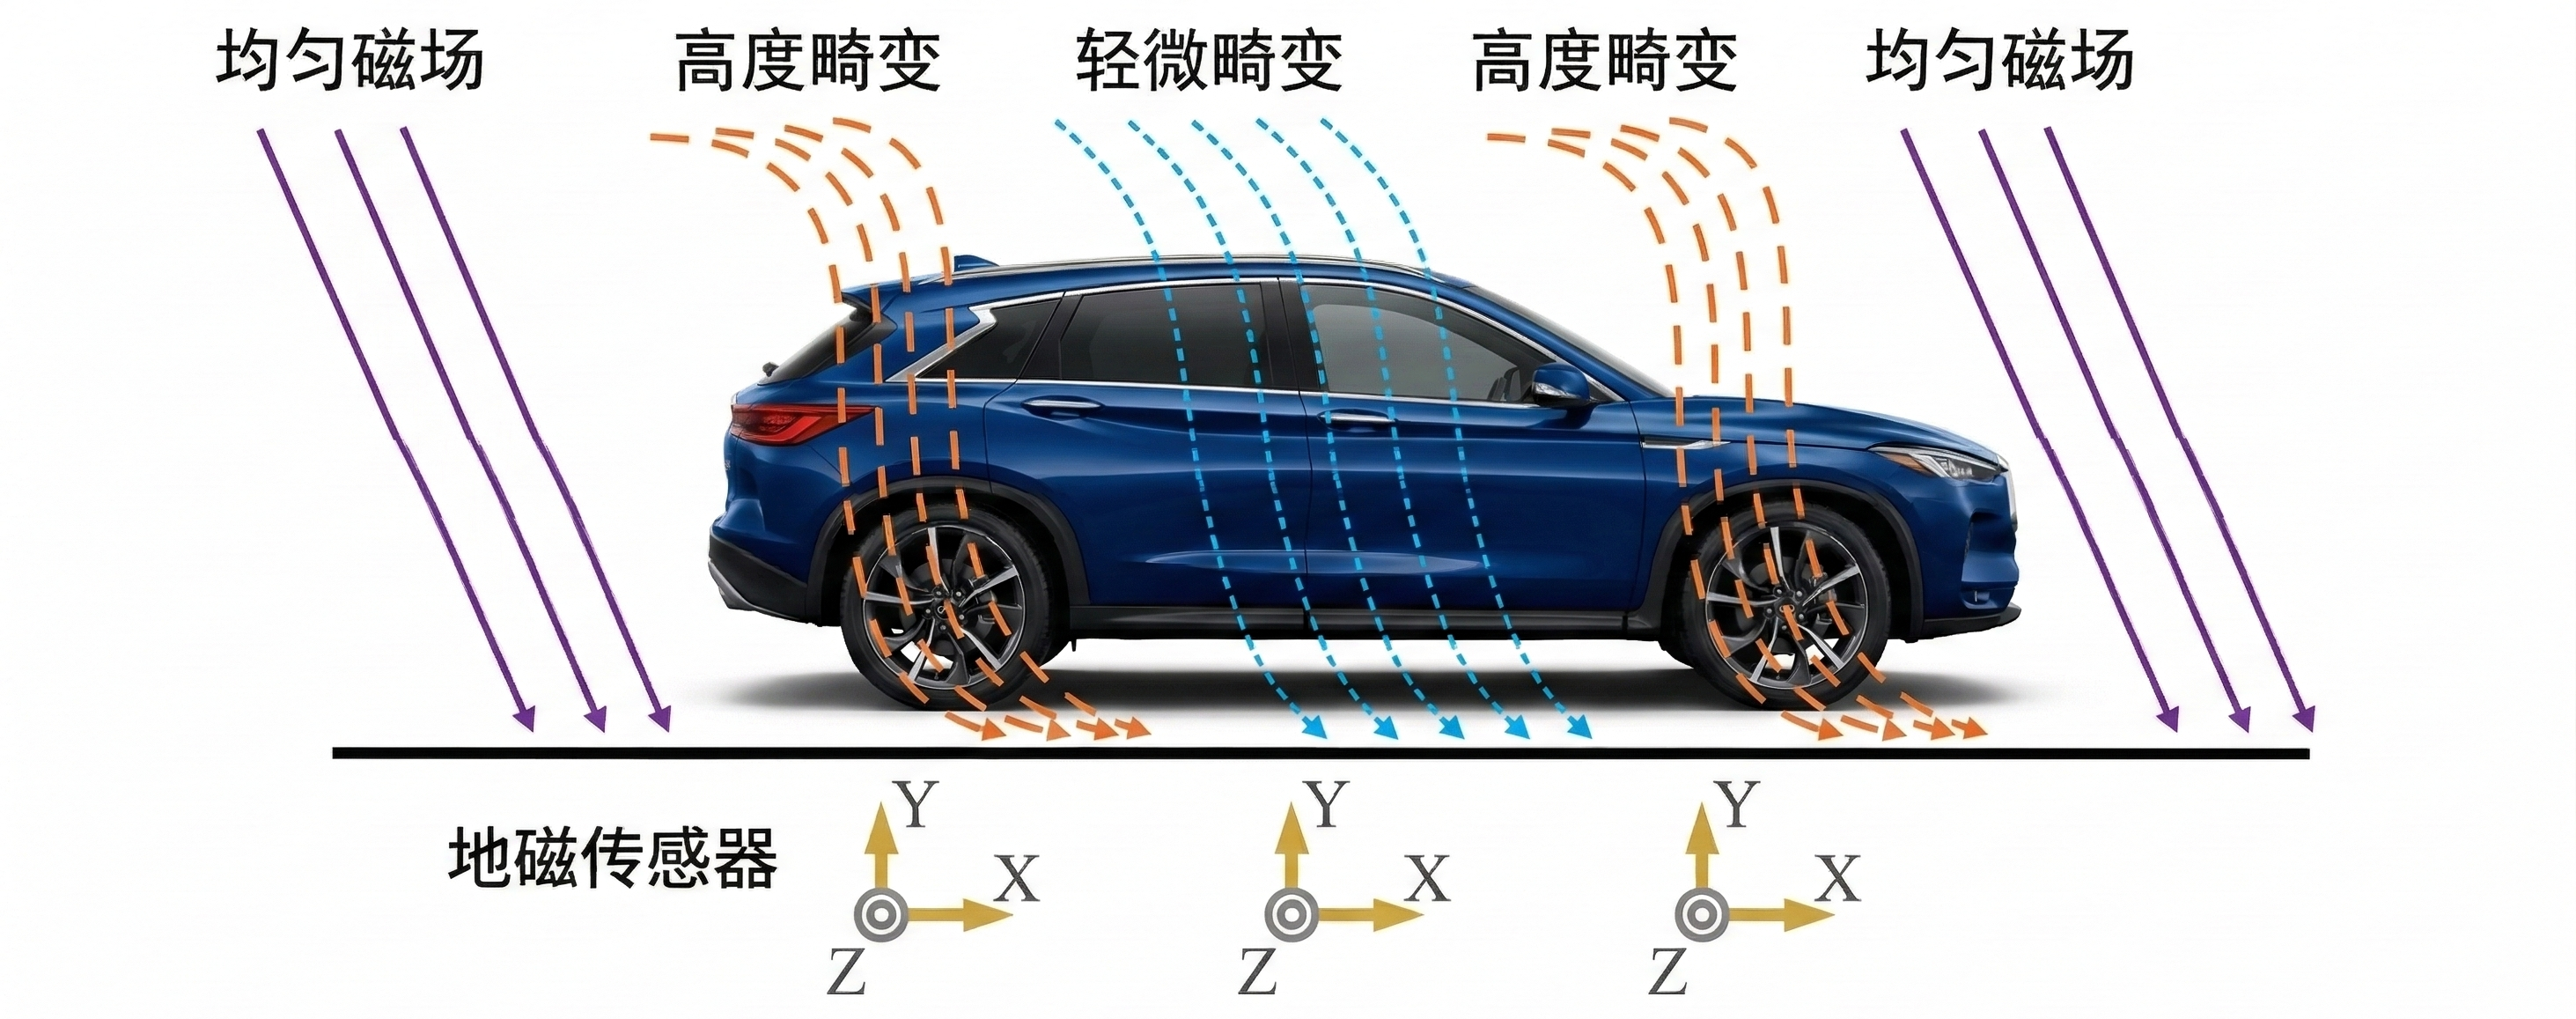
\includegraphics[width=0.85\textwidth]{images/chapter2/fig_2_1_mag_disturbance}
	\caption{车辆引起磁场扰动示意图}
	\label{fig:mag_disturbance}
\end{figure}

在上述机理基础上，空间磁场畸变会表现为传感器输出相对无车时基线磁场值的一段明显扰动。如图~\ref{fig:mag_value}所示，当车辆经过传感器时，磁场强度数据会在原有基线附近出现显著偏移，并形成具有一定持续时间的扰动区间；当车辆驶离后，输出值再逐步恢复并重新稳定在基线附近。基于这一扰动过程，可以进一步提取车辆触发时刻、持续时长以及磁场扰动峰值等检测信息。结合多地磁传感器观测，这些特征还可为后续的车辆跨点匹配、交通参数估计以及车辆类型判别等上层处理提供基础输入。

\begin{figure}[htbp]
	\centering
	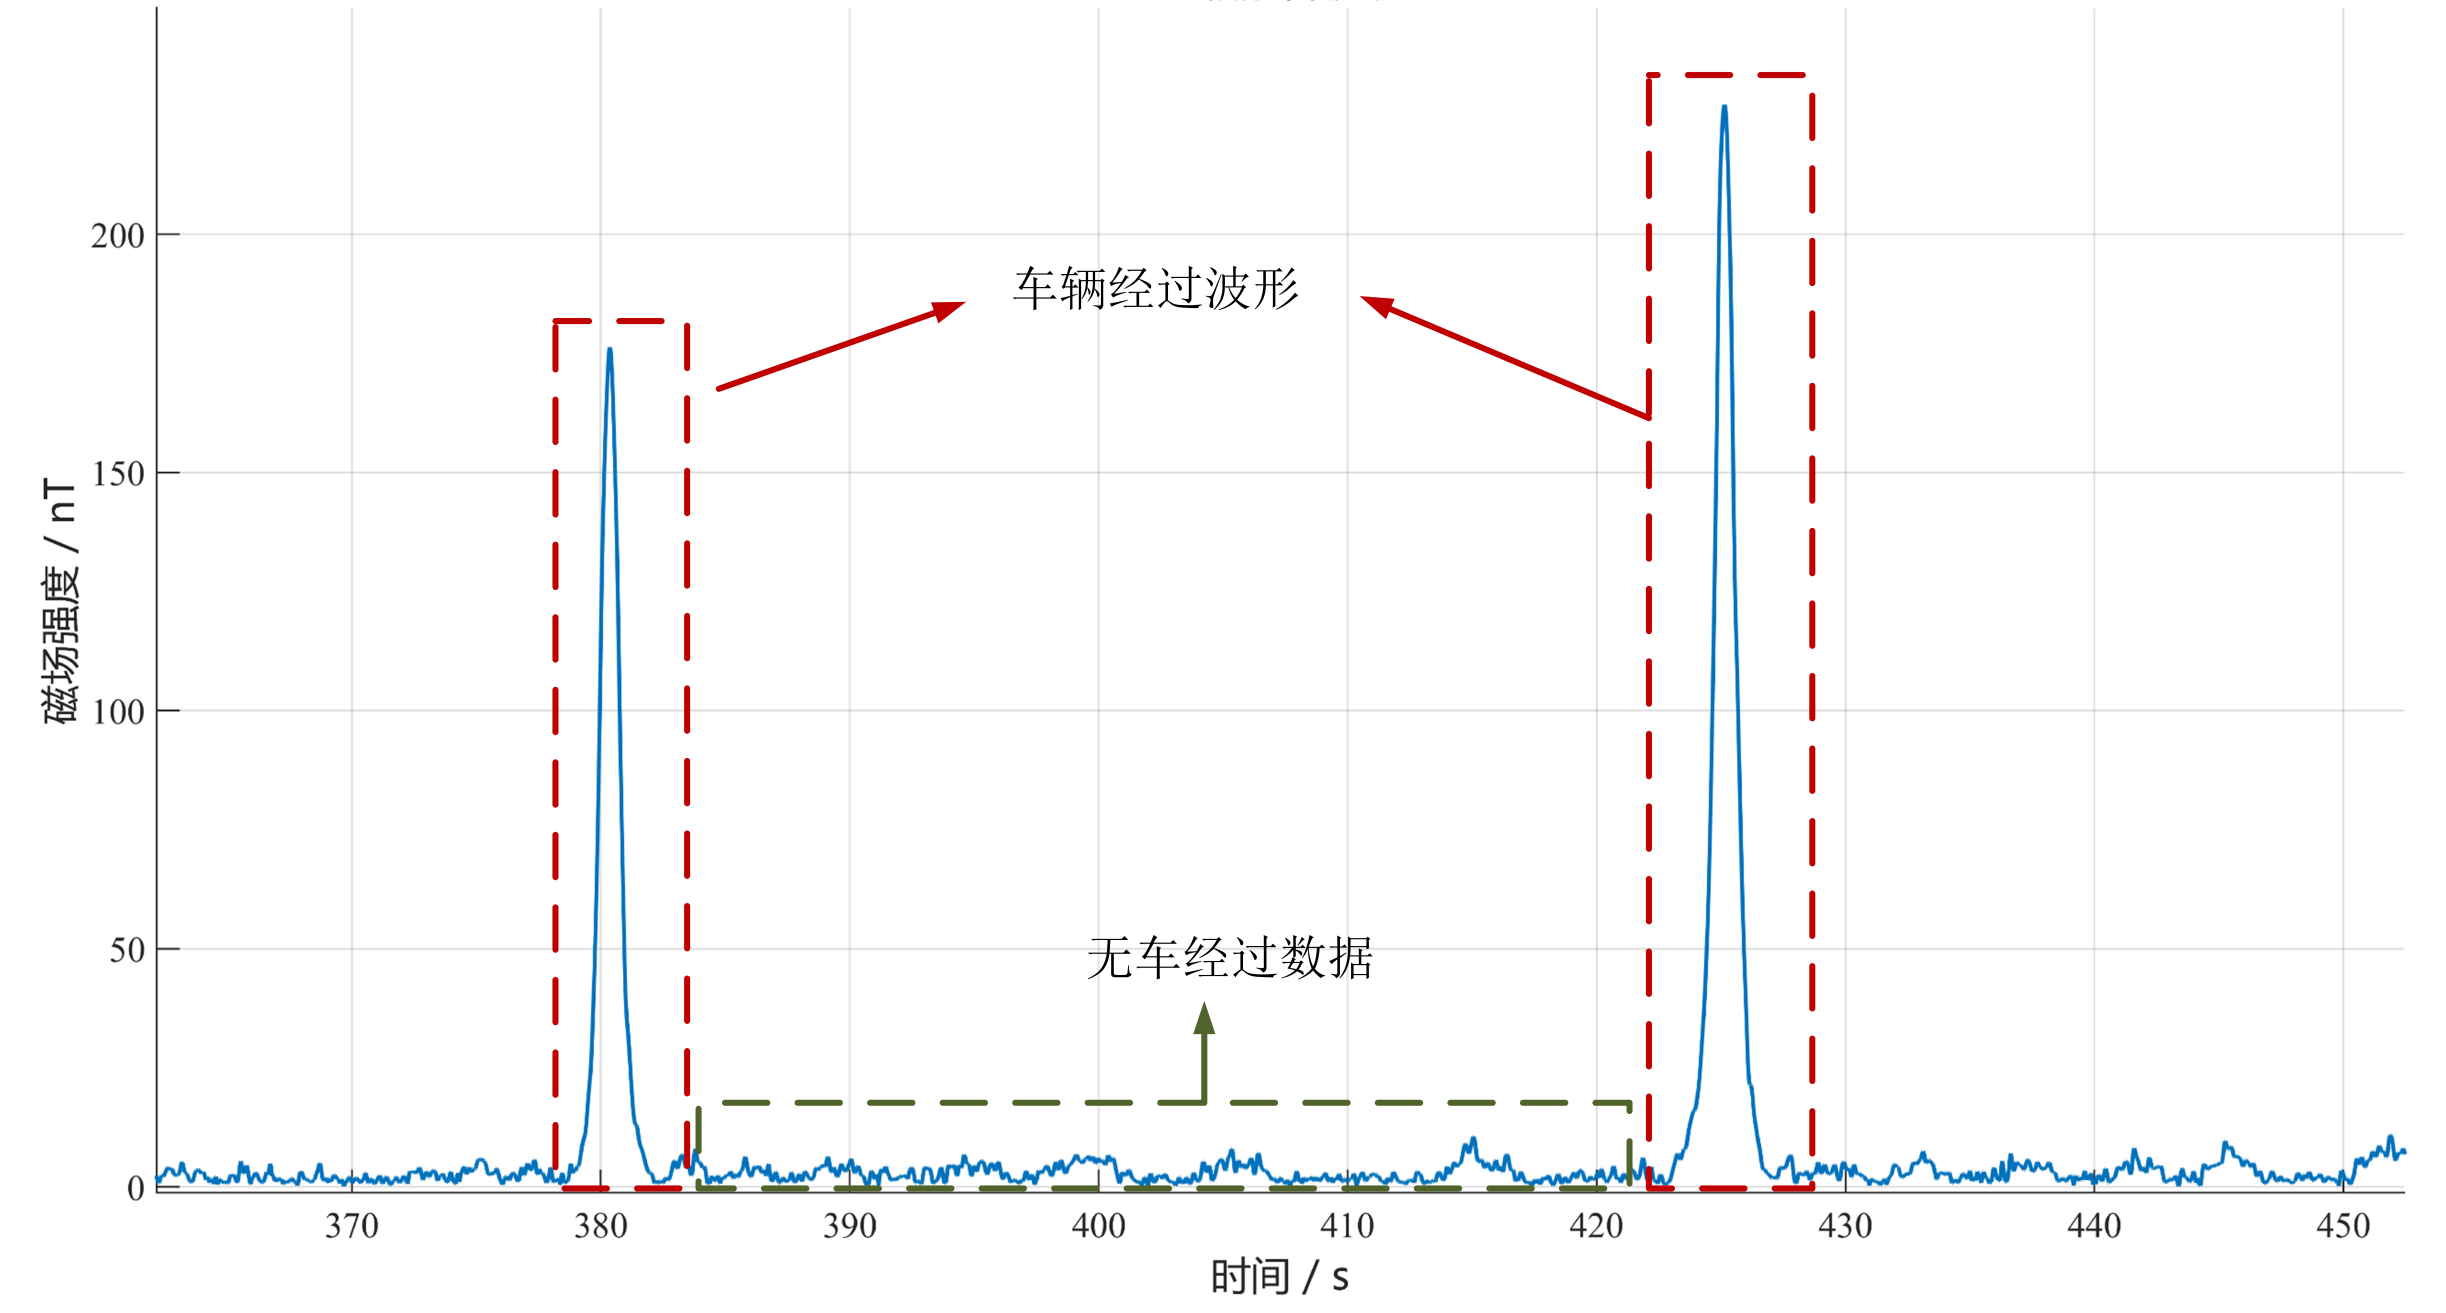
\includegraphics[width=0.85\textwidth]{images/chapter2/fig_2_2_mag_value}
	\caption{车辆经过时地磁传感器检测的磁场强度数据变化图}
	\label{fig:mag_value}
\end{figure}

同时需要指出的是，地磁扰动还具有明显的空间衰减特性。随着车辆与地磁传感器横向距离的增大，传感器接收到的扰动幅值会逐渐减小，信噪比也随之下降；再叠加环境噪声和基线波动等因素的影响，车辆通过所引起的磁场变化可能不再显著，从而导致漏检现象的出现。

\subsection{地磁车辆检测算法}\label{sec:vehicle_detection}

地磁车辆检测的任务是在连续三轴磁场采样序列中识别由车辆通过引起的扰动区间，并在基线缓慢漂移与随机噪声叠加条件下保持触发稳定。不同系统在采样频率、特征构造和上报字段上存在差异，但基本处理流程较为一致：先对原始观测进行平滑去噪并在线估计无车基线，再将三轴相对基线的偏移量转换为标量检测统计量，最后通过阈值或状态机判决确定车辆是否进入和离开传感器有效作用范围，并据此生成检测数据\cite{ding2004signalprocessing,sarcevic2022singlemagnetometer}。

为便于统一判决，设传感器在第 $q$ 个采样时刻的三轴磁场观测向量和对应的标量检测统计量分别为：
\begin{equation}
	\mathbf{B}(q)=
	\begin{bmatrix}
		B_x(q)\\
		B_y(q)\\
		B_z(q)
	\end{bmatrix}
	\label{eq:ch2_mag_observation_vector}
\end{equation}
\begin{equation}
	d(q)=\left\lVert \mathbf{B}(q)-\bar{\mathbf{B}}(q)\right\rVert_2
	\label{eq:ch2_mag_detection_scalar}
\end{equation}
其中，$B_x(q)$、$B_y(q)$、$B_z(q)$ 分别表示 $x$、$y$、$z$ 三个轴向的磁场分量观测值；$\bar{\mathbf{B}}(q)$ 表示对应时刻的无车基线估计向量，通常由滑动平均、低通滤波或递推估计获得。式~\eqref{eq:ch2_mag_detection_scalar}实质上是将三个轴向相对基线的偏移量融合为一个标量，用于表征当前采样时刻整体磁场扰动强度。这样，无论扰动主要体现在哪个轴向上，都可以在同一尺度下进行比较和阈值判决。由于 $d(q)$ 会随车型、车速、车辆相对传感器的通过位置以及姿态等因素产生幅值波动，同时基线也可能随温度或环境磁背景变化而缓慢漂移，因此检测阶段通常需要采用阈值自适应或引入序列一致性约束，以降低长期部署中阈值失配与抖动触发带来的稳定性下降\cite{sarcevic2022singlemagnetometer}。

在判决逻辑上，阈值判决通过比较 $d(q)$ 与阈值 $T$ 实现二值判定：当 $d(q)>T$ 时判为有车，否则判为无车，其中 $T$ 为判决阈值。该方法结构简单、计算代价低，适合在传感器端实时运行，但固定阈值对幅值变化与基线漂移较为敏感。为提升不同工况下的可用性，可采用自适应阈值策略，根据近期噪声水平或统计量分布对 $T$ 进行在线更新，从而在车辆幅值变化或背景波动时维持较稳定的检出性能。

仅依赖逐点阈值比较时，检测统计量 \(d(q)\) 在阈值附近的波动可能引发重复触发或短脉冲误检。为减小这类影响，工程实现中常在阈值判决基础上引入有限状态机（Finite State Machine, FSM）判决机制。如图~\ref{fig:ch2_fsm_detection}所示，FSM 将检测过程划分为无车状态 \(s_0\)、进入确认状态 \(s_1\)、有车状态 \(s_2\) 和离开确认状态 \(s_3\) 四个状态。记 \(T_{on}\) 和 \(T_{off}\) 分别为车辆进入判决阈值和车辆离开判决阈值，\(N_{in}\) 和 \(N_{out}\) 分别为进入确认和离开确认所需的连续采样点数。当 \(d(q)>T_{on}\) 时，系统由无车状态转入进入确认状态；当进入条件连续满足 \(N_{in}\) 个采样点时，确认车辆进入并转入有车状态。当 \(d(q)<T_{off}\) 时，系统进入离开确认状态；当离开条件连续满足 \(N_{out}\) 个采样点时，确认车辆离开并输出检测结果。该机制可避免统计量在阈值附近短时波动时频繁切换状态，从而提高对噪声和突发干扰的容忍度。在多车道场景下，还可进一步结合多轴一致性、滞回阈值或车道约束等机制，降低相邻车道干扰引发的误检概率\cite{guilbert2016statemachine}。

\begin{figure}[htbp]
	\centering
	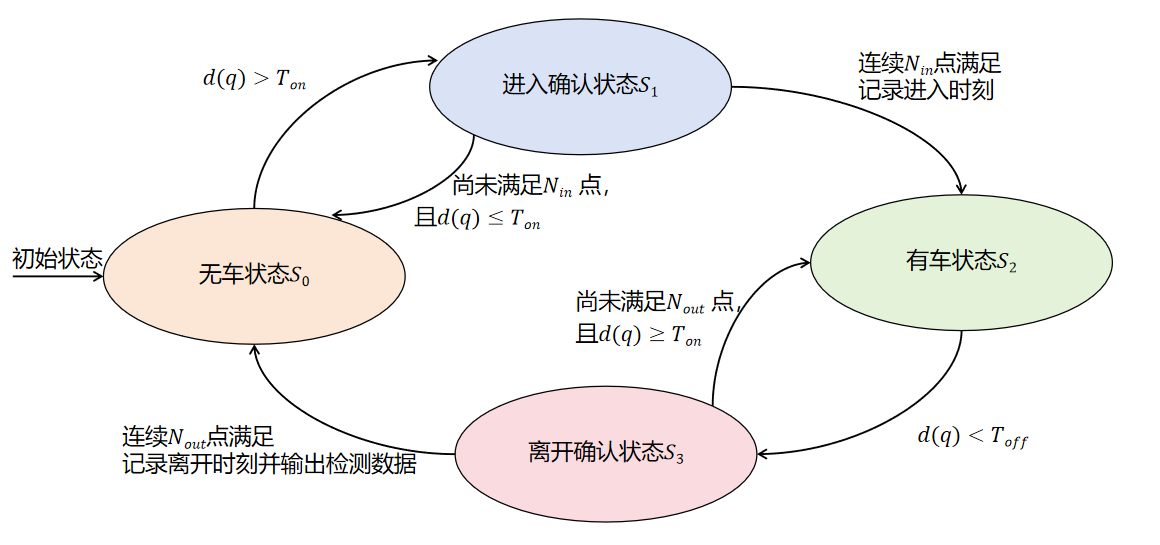
\includegraphics[width=0.82\textwidth]{images/chapter2/fig_2_3_fsm_detection}
	\caption{FSM状态机判决示意图}
	\label{fig:ch2_fsm_detection}
\end{figure}

当进入时刻和离开时刻被稳定确定后，系统即可生成一条车辆检测数据。该数据通常以进入时刻和离开时刻表征车辆在地磁传感器有效探测区内的通过区间，并可进一步输出扰动峰值、持续时长等特征字段，为速度估计、占有率计算、车长推断以及跨点数据关联提供基础量测输入\cite{balid2018intelligent}。


\section{卡尔曼滤波算法}

由于存在杂波干扰以及传感器量测误差，传感器输出与目标真实状态之间通常会有偏差，因此需要借助滤波算法对目标状态进行估计，以减弱不确定性带来的影响。卡尔曼滤波是多目标跟踪中常用的滤波方法之一，主要适用于线性动态系统。其基本思想是先依据目标运动模型对下一时刻状态进行预测，再将预测结果与传感器量测进行加权融合，从而得到目标运动状态的估计。该方法计算复杂度相对较低，并且在线性系统中能够取得较为稳定的跟踪效果。


\subsection{卡尔曼滤波算法的过程}

卡尔曼滤波的递推过程可以概括为模型建立、状态预测和量测更新三个步骤。为便于说明，先给出离散时间系统的状态方程与观测方程：
\begin{equation}
	x(k)=F(k-1)x(k-1)+W(k-1)
\end{equation}
\begin{equation}
	z(k)=H(k)x(k)+V(k)
\end{equation}

其中，$x(k)$ 表示 $k$ 时刻目标的运动状态，$F(k-1)$ 为目标的状态转移矩阵，$W(k-1)$ 为系统的过程噪声；$z(k)$ 表示 $k$ 时刻的量测，$H(k)$ 为系统的观测矩阵，$V(k)$ 为系统的量测噪声。

通常假设过程噪声与量测噪声相互独立，且均服从均值为零的高斯分布，则有：
\begin{equation}
	E\!\left(W(k)W^{T}(j)\right)=Q(k)\delta_{kj}
\end{equation}
\begin{equation}
	E\!\left(V(k)V^{T}(j)\right)=R(k)\delta_{kj}
\end{equation}
\begin{equation}
	E\!\left(W(k)V^{T}(j)\right)=0
\end{equation}

其中，$Q(k)$ 为 $k$ 时刻系统过程噪声的协方差矩阵，$R(k)$ 为 $k$ 时刻系统量测噪声的协方差矩阵。$\delta_{kj}$ 为 Kronecker delta 函数，其定义为：
\begin{equation}
	\delta_{kj}=
	\begin{cases}
		1, & k=j\\
		0, & k\neq j
	\end{cases}
\end{equation}

在完成上述建模后，卡尔曼滤波在每一个采样时刻均按照递推方式运行。具体而言，先利用上一时刻的状态估计结果对当前时刻的目标状态进行预测，再结合当前时刻获得的量测对预测结果进行修正。

首先，状态预测步骤利用 $k-1$ 时刻的后验估计得到 $k$ 时刻的先验状态预测，其计算公式为：
\begin{equation}
	\hat{x}(k|k-1)=F(k-1)\hat{x}(k-1|k-1)
\end{equation}
\begin{equation}
	P(k|k-1)=F(k-1)P(k-1|k-1)F^{T}(k-1)+Q(k-1)
\end{equation}

其中，$\hat{x}(k|k-1)$ 表示利用 $k-1$ 时刻信息得到的 $k$ 时刻目标状态预测，$P(k|k-1)$ 为对应的状态预测协方差矩阵。

在获得先验预测后，当 $k$ 时刻量测 $z(k)$ 到达时，需要将其与预测结果进行融合，以得到更优的后验估计。为此，首先定义新息向量：
\begin{equation}
	\nu(k)=z(k)-H(k)\hat{x}(k|k-1)
\end{equation}
其中，新息反映了当前量测与预测量测之间的偏差。对应的新息协方差矩阵为：
\begin{equation}
	S(k)=H(k)P(k|k-1)H^{T}(k)+R(k)
\end{equation}

进一步可得卡尔曼滤波增益：
\begin{equation}
	K(k)=P(k|k-1)H^{T}(k)S^{-1}(k)
\end{equation}

由此即可完成量测更新，得到 $k$ 时刻目标运动状态的后验估计及其协方差：
\begin{equation}
	\hat{x}(k|k)=\hat{x}(k|k-1)+K(k)\nu(k)
\end{equation}
\begin{equation}
	P(k|k)=P(k|k-1)-K(k)H(k)P(k|k-1)
\end{equation}

其中，$\hat{x}(k|k)$ 为 $k$ 时刻目标运动状态的后验估计，$P(k|k)$ 为对应的状态估计协方差矩阵。

由上述过程可见，卡尔曼滤波通过状态预测和量测更新的交替执行，实现了对目标运动状态的递推估计。其中，预测步骤依据目标运动规律给出目标状态的先验结果，更新步骤则利用当前量测对其进行修正，从而在含噪环境下获得更加稳定和准确的状态估计。卡尔曼滤波器的性能在很大程度上取决于目标运动模型的选取。下面介绍卡尔曼滤波器中常见的运动模型及其过程噪声的选取。

\subsection{目标运动模型}

卡尔曼滤波以及大多数跟踪器都建立在目标运动模型的基础上。目标运动模型描述了目标运动状态随时间的变化规律，选择合适的目标运动模型有助于提高目标状态估计的准确性。根据目标的运动学特征，常见的目标运动模型包括常速度（Constant Velocity，CV）模型、常加速度（Constant Acceleration，CA）模型以及匀速转弯（Constant Turn，CT）模型等。


\textnormal{（1）CV 模型}\par\vspace{0.3\baselineskip}

常速度模型假设目标做匀速直线运动。在理想情况下，目标加速度应为零；但在实际应用中，受外界干扰影响，加速度通常不可能严格为零。因此，CV 模型将加速度视为均值为零的高斯白噪声，用来描述这部分扰动

状态转移矩阵为：
\begin{equation}
	F(k)=
	\begin{bmatrix}
		1 & T_k\\
		0 & 1
	\end{bmatrix}
\end{equation}

噪声增益向量为：
\begin{equation}
	\Gamma(k)=
	\begin{bmatrix}
		\dfrac{1}{2}T_k^2\\
		T_k
	\end{bmatrix}
\end{equation}

过程噪声的协方差矩阵为：
\begin{equation}
	Q(k)=\Gamma(k)\sigma_w^2\Gamma^{T}(k)=
	\begin{bmatrix}
		\dfrac{1}{4}T_k^4 & \dfrac{1}{2}T_k^3\\[6pt]
		\dfrac{1}{2}T_k^3 & T_k^2
	\end{bmatrix}\sigma_w^2
\end{equation}

其中，$T_k$ 为 $k-1$ 时刻与 $k$ 时刻之间的时间间隔，$\sigma_w$ 表示过程噪声的标准差。在实际使用中，CV 模型中 $\sigma_w$ 的取值通常与目标最大加速度 $a_M$ 的数量级有关，一般可取\(0.5a_M \leq \sigma_w \leq a_M\)\cite{barshalom2004estimation}。


由此可见，CV 模型结构简单、参数较少，适合描述运动状态较为平稳的目标；但当目标存在较明显的加减速行为时，仅采用 CV 模型往往难以准确刻画其运动过程。

\textnormal{（2）CA 模型}\par\vspace{0.3\baselineskip}

当目标在运动过程中存在较明显的加速或减速行为时，常加速度模型能够更好地描述其状态变化。CA 模型假设目标在相邻采样间隔内保持恒定加速度，而加速度的变化部分由均值为零的白噪声来表征。等价地说，该模型认为加速度满足离散时间维纳过程。以下仍以目标在一维空间中的运动为例，其状态向量由位置、速度和加速度共同构成。

状态转移矩阵为：
\begin{equation}
	F(k)=
	\begin{bmatrix}
		1 & T_k & \dfrac{T_k^2}{2}\\
		0 & 1   & T_k\\
		0 & 0   & 1
	\end{bmatrix}
\end{equation}

噪声增益向量为：
\begin{equation}
	\Gamma(k)=
	\begin{bmatrix}
		\dfrac{T_k^2}{2}\\
		T_k\\
		1
	\end{bmatrix}
\end{equation}

过程噪声的协方差矩阵为：
\begin{equation}
	Q(k)=\Gamma(k)\sigma_q^2\Gamma^{T}(k)=
	\begin{bmatrix}
		\dfrac{1}{4}T_k^4 & \dfrac{1}{2}T_k^3 & \dfrac{1}{2}T_k^2\\[6pt]
		\dfrac{1}{2}T_k^3 & T_k^2 & T_k\\[6pt]
		\dfrac{1}{2}T_k^2 & T_k & 1
	\end{bmatrix}\sigma_q^2
\end{equation}

其中，$\sigma_q$ 表示过程噪声的标准差。在实际应用中，CA 模型中 $\sigma_q$ 的取值通常与两次更新时刻之间目标最大加速度增量 $\Delta a_M$ 的数量级有关，一般可取\(0.5\Delta a_M \leq \sigma_q \leq \Delta a_M\)\cite{barshalom2004estimation}：

与 CV 模型相比，CA 模型能够更好地反映目标速度随时间变化的过程，因此更适合处理存在明显加减速机动的目标。但与此同时，CA 模型的状态维数更高，对模型参数设置也更加敏感。

\textnormal{（3）CT 模型}\par\vspace{0.3\baselineskip}

当目标存在明显转弯机动时，仅采用直线运动模型往往难以获得理想的状态预测结果，此时可采用匀速转弯模型进行描述。CT 模型主要用于刻画目标在二维平面内以近似恒定角速度转弯的运动状态。该模型通过引入转弯角速度，使状态转移过程能够反映目标方向变化对位置和速度的影响。

令 $\omega$ 表示目标的转弯角速度，在二维坐标系中，目标的状态向量为：
\[
x(k)=[x,\ v_x,\ y,\ v_y]^T
\]
则 CT 模型的离散状态方程为：
\begin{equation}
	x(k+1)=
	\begin{bmatrix}
		1 & \dfrac{\sin \omega T}{\omega} & 0 & -\dfrac{1-\cos \omega T}{\omega}\\[8pt]
		0 & \cos \omega T & 0 & -\sin \omega T\\[6pt]
		0 & \dfrac{1-\cos \omega T}{\omega} & 1 & \dfrac{\sin \omega T}{\omega}\\[8pt]
		0 & \sin \omega T & 0 & \cos \omega T
	\end{bmatrix}
	x(k)
	+
	\begin{bmatrix}
		\dfrac{T^2}{2}\\
		T\\
		\dfrac{T^2}{2}\\
		T
	\end{bmatrix}
	w(k)
\end{equation}

其中，$T$ 为相邻时刻之间的时间间隔，$w(k)$ 为过程噪声。目标转弯角速度 $\omega$ 决定了目标的转弯速度和转弯方向，因此 CT 模型能够较好地描述存在持续转向行为的机动目标。在实际应用中，应结合具体场景和目标运动特性选择合适的运动模型，从而为后续状态估计提供更准确的预测基础。



\section{数据关联算法}\label{sec:orm}

在多目标跟踪中，滤波器可以依据历史信息给出各条轨迹在下一时刻的预测状态，但当前到来的量测并不携带目标身份，因此仍需判断每个量测应由哪条轨迹吸收更新。若关联错误，错误量测会直接进入状态更新过程，继而引起轨迹漂移、身份切换甚至轨迹中断。因此，数据关联的核心任务不是简单地为每条轨迹寻找距离最近的量测，而是在漏检、杂波同时存在的条件下，为轨迹选择最合理的更新对象。

设更新时刻为 $k$，当前共有 $N_k$ 条待更新轨迹，接收到的量测集合记为：
\begin{equation}
	\mathcal{Z}_k=
	\left\{
	z^{(1)}(k),z^{(2)}(k),\ldots,z^{(M_k)}(k)
	\right\}
\end{equation}
式中，$\mathcal{Z}_k$ 表示 $k$ 时刻的量测集合，$M_k$ 表示当前时刻的量测数，$z^{(j)}(k)$ 表示第 $j$ 个量测。对第 $i$ 条轨迹，滤波器已给出预测状态 $\hat{x}^{(i)}(k|k-1)$ 和预测协方差 $P^{(i)}(k|k-1)$。数据关联要解决的问题，就是判断 $\mathcal{Z}_k$ 中哪些量测可以用于更新第 $i$ 条轨迹，哪些量测应视为杂波或新目标候选。接下来将对数据关联过程中的常用算法进行相关介绍。


\subsection{最近邻类数据关联方法}


最近邻数据关联方法（Nearest Neighbor Data Association, NNDA）是实现最为直接的一类关联方法，在部分文献中也称为最近邻滤波方法\cite{sea1971suboptimal}。其基本思想是，先依据轨迹预测状态构造跟踪门，排除明显不可能的轨迹量测组合，再从门内候选量测中选取与当前轨迹最接近的一个进行更新。由于该方法只保留一个候选量测，因此计算简单，适合实时性要求较高且目标密度较低的场景。

在前文线性观测模型下，轨迹 $i$ 在时刻 $k$ 的预测量测可写为：
\begin{equation}
	\hat{z}^{(i)}(k|k-1)
	=
	H(k)\hat{x}^{(i)}(k|k-1)
\end{equation}
对应的新息协方差为：
\begin{equation}
	S^{(i)}(k)
	=
	H(k)P^{(i)}(k|k-1)H^{T}(k)
	+
	R(k)
\end{equation}
式中，$\hat{z}^{(i)}(k|k-1)$ 表示轨迹 $i$ 的预测量测，$H(k)$ 表示量测矩阵，$\hat{x}^{(i)}(k|k-1)$ 表示轨迹 $i$ 的预测状态，$S^{(i)}(k)$ 表示轨迹 $i$ 的新息协方差，$P^{(i)}(k|k-1)$ 表示轨迹 $i$ 的预测协方差，$R(k)$ 表示量测噪声协方差矩阵。

进一步定义轨迹 $i$ 与量测 $j$ 的新息向量为：
\begin{equation}
	\nu^{(i,j)}(k)
	=
	z^{(j)}(k)-\hat{z}^{(i)}(k|k-1)
\end{equation}
轨迹 $i$ 与量测 $j$ 之间的平方马氏距离为：
\begin{equation}
	d_k^2(i,j)
	=
	\left(
	\nu^{(i,j)}(k)
	\right)^{T}
	\left(
	S^{(i)}(k)
	\right)^{-1}
	\nu^{(i,j)}(k)
\end{equation}
相应的落入轨迹 $i$ 跟踪门内的量测编号集合可写为：
\begin{equation}
	\mathcal{G}^{(i)}_k
	=
	\left\{
	j \mid d_k^2(i,j)\le \gamma
	\right\}
\end{equation}
式中，$\gamma$ 表示跟踪门阈值,若量测维数为 $m$，通常可取 $\gamma=\chi_m^2(P_G)$，其中，$\chi_m^2(\cdot)$ 表示自由度为 $m$ 的卡方分布分位函数，$P_G$ 表示真实量测被跟踪门保留的概率。

在只针对单条轨迹作局部选择时，最近邻方法取平方马氏距离最小的量测作为更新对象，即：
\begin{equation}
	j_i^\star
	=
	\arg\min_{j\in\mathcal{G}^{(i)}_k}
	d_k^2(i,j)
\end{equation}
式中，$j_i^\star$ 表示与轨迹 $i$ 关联的最近邻量测编号。若 $\mathcal{G}^{(i)}_k=\varnothing$，则认为轨迹 $i$ 在当前时刻未检出可关联量测；否则可按
\begin{equation}
	\hat{x}^{(i)}(k|k)
	=
	\hat{x}^{(i)}(k|k-1)
	+
	K^{(i)}(k)\nu^{(i,j_i^\star)}(k)
\end{equation}
完成状态更新。式中，$\hat{x}^{(i)}(k|k)$ 表示更新后的状态估计，$K^{(i)}(k)$ 表示轨迹 $i$ 在时刻 $k$ 的卡尔曼增益，$\nu^{(i,j_i^\star)}(k)$ 表示最近邻量测对应的新息向量。

上述形式只针对单条轨迹在各自跟踪门内作局部最近邻选择。若进一步考虑多条轨迹之间对同一批候选量测的竞争关系，则最近邻思想可推广为全局最近邻（Global Nearest Neighbor, GNN）关联方法。GNN 不再对各条轨迹分别独立选择最近量测，而是在当前时刻同时考虑所有轨迹和所有候选量测之间的匹配关系，在满足一对一约束的条件下求取总代价最小的关联结果，因此具有实现直接、求解高效、工程部署方便等优点，在实时性要求较高的系统中仍被广泛采用\cite{kuhn1955hungarian,wang2022improvedgnn}。

在给定跟踪门候选集合后，可先定义轨迹 $i$ 与量测 $j$ 的关联代价：
\begin{equation}
	Cost_{i,j}
	=
	\begin{cases}
		d_k^2(i,j), & j\in\mathcal{G}^{(i)}_k\\
		C_{\max}, & j\notin\mathcal{G}^{(i)}_k
	\end{cases}
\end{equation}
式中，$Cost_{i,j}$ 表示轨迹 $i$ 与量测 $j$ 的关联代价，$Cost_{\max}$ 表示一个足够大的惩罚值，用于排除不在跟踪门内的不合理匹配。令二值分配变量 $a_{i,j}$ 表示量测 $j$ 是否分配给轨迹 $i$，则 GNN 的单时刻线性分配模型可写为：
\begin{align}
	\min_{\{a_{i,j}\}}\quad
	& \sum_{i=1}^{N_k}\sum_{j=1}^{M_k} Cost_{i,j}a_{i,j} \\
	\text{s.t.}\quad
	& a_{i,j}\in\{0,1\}, \\
	& \sum_{j=1}^{M_k} a_{i,j}\le 1,\qquad i=1,2,\ldots,N_k, \\
	& \sum_{i=1}^{N_k} a_{i,j}\le 1,\qquad j=1,2,\ldots,M_k.
\end{align}
式中，$a_{i,j}=1$ 表示量测 $j$ 分配给轨迹 $i$，$a_{i,j}=0$ 表示二者不关联。目标函数表示在所有可行匹配中寻找总代价最小的分配方案；第一组约束表示每条轨迹至多分配一个量测，第二组约束表示每个量测至多分配给一条轨迹。该问题本质上是标准线性指派问题，通常可用匈牙利算法高效求解。对未被分配量测的轨迹，可视为当前时刻漏检；对未被分配的量测，则可作为新目标候选。

总体来看，NNDA 与 GNN 都属于当前时刻直接给出唯一匹配结果的硬关联方法。前者实现更简洁，后者则显式处理了多轨迹之间的一对一竞争关系；但二者都可能在信息不足时把局部误配直接带入状态更新过程。为减弱这种硬判决带来的直接冲击，可进一步采用概率数据关联方法。

\subsection{概率数据关联方法}

当某条轨迹的跟踪门内同时出现多个都较为合理的候选量测时，无论是 NNDA 还是 GNN，都需要在当前时刻直接给出唯一分配。若当前信息不足以消除歧义，这种硬判决容易把局部误配直接传递到状态更新阶段。为此，概率数据关联方法不急于只选取一个量测，而是先对候选关联事件进行概率化建模，再按关联概率完成更新。


概率数据关联方法（Probabilistic Data Association, PDA）主要面向单条轨迹的关联更新问题。其基本思想是先为门内候选量测计算关联概率，再按概率加权完成状态更新\cite{barshalom1975pda,chen2018weightedpda}。

对于任意 $j\in\mathcal{G}^{(i)}_k$，其量测似然可写为：
\begin{equation}
	L_{i,j}
	=
	\mathcal{N}
	\left(
	z^{(j)}(k);
	\hat{z}^{(i)}(k|k-1),
	S^{(i)}(k)
	\right)
\end{equation}
式中，$L_{i,j}$ 表示量测 $j$ 由轨迹 $i$ 生成的似然值，$\mathcal{N}(\cdot;\mu,\Sigma)$ 表示均值为 $\mu$、协方差为 $\Sigma$ 的高斯概率密度函数。

在考虑漏检和杂波后，PDA 常用的关联概率写为：
\begin{equation}
	\beta_{i,j}
	=
	\frac{P_D L_{i,j}}
	{\lambda_c V_k^{(i)}+P_D\sum\limits_{\ell\in\mathcal{G}^{(i)}_k}L_{i,\ell}}
\end{equation}
对应的漏检概率为：
\begin{equation}
	\beta_{i,0}
	=
	1-\sum_{j\in\mathcal{G}^{(i)}_k}\beta_{i,j}
\end{equation}
式中，$\beta_{i,j}$ 表示量测 $j$ 与轨迹 $i$ 的关联概率，$\beta_{i,0}$ 表示轨迹 $i$ 在当前时刻漏检的概率，$P_D$ 表示检测概率，$\lambda_c$ 表示杂波空间密度，$V_k^{(i)}$ 表示轨迹 $i$ 在时刻 $k$ 的跟踪门体积，$\ell$ 为跟踪门内量测的求和下标。

得到关联概率后，可构造加权新息：
\begin{equation}
	\bar{\nu}^{(i)}(k)
	=
	\sum_{j\in\mathcal{G}^{(i)}_k}
	\beta_{i,j}\nu^{(i,j)}(k)
\end{equation}
再完成状态更新：
\begin{equation}
	\hat{x}^{(i)}(k|k)
	=
	\hat{x}^{(i)}(k|k-1)
	+
	K^{(i)}(k)\bar{\nu}^{(i)}(k)
\end{equation}
式中，$\bar{\nu}^{(i)}(k)$ 表示轨迹 $i$ 的加权新息，$\hat{x}^{(i)}(k|k)$ 表示更新后的状态估计，$K^{(i)}(k)$ 表示轨迹 $i$ 的卡尔曼增益。由上式可见，PDA 通过对门内候选量测进行概率加权，减弱了单个错误匹配对状态估计的冲击，因此在单轨迹场景下通常比硬关联方法更稳健。

需要指出的是，PDA 默认各条轨迹之间相互独立。当多条轨迹共用同一批门内量测时，若仍分别独立计算关联概率，可能出现同一量测被多条轨迹同时高权重使用的情况。为进一步处理多轨迹之间的量测互斥关系，需要引入联合概率数据关联方法。


联合概率数据关联方法（Joint Probabilistic Data Association, JPDA）是 PDA 在多目标场景下的自然扩展。它不再只考虑单条轨迹内部的候选量测竞争关系，而是从整体上描述多条轨迹与多条量测的联合匹配状态，再由联合假设的后验概率计算单条轨迹的边缘关联概率，从而避免同一量测被多条轨迹同时高权重使用\cite{fortmann1983jpda,cheng1998fastjpda}。

定义时刻 $k$ 的联合关联变量为：
\begin{equation}
	\theta_k
	=
	\left[
	\theta_k^{(1)},\theta_k^{(2)},\ldots,\theta_k^{(N_k)}
	\right]^{T}
\end{equation}
式中，$\theta_k$ 表示当前时刻的联合关联变量，$\theta_k^{(i)}=j$ 表示轨迹 $i$ 与量测 $j$ 关联，$\theta_k^{(i)}=0$ 表示轨迹 $i$ 在当前时刻漏检，$N_k$ 表示待更新轨迹数。设 $\Theta_k$ 为满足一对一约束的可行联合假设集合，则轨迹 $i$ 与量测 $j$ 的边缘关联概率可写为：
\begin{equation}
	\beta_{i,j}
	=
	\sum_{\theta_k\in\Theta_k:\,\theta_k^{(i)}=j}
	p\!\left(
	\theta_k\mid\mathcal{Z}_k
	\right)
\end{equation}
对应的漏检概率为：
\begin{equation}
	\beta_{i,0}
	=
	\sum_{\theta_k\in\Theta_k:\,\theta_k^{(i)}=0}
	p\!\left(
	\theta_k\mid\mathcal{Z}_k
	\right)
\end{equation}
式中，$\beta_{i,j}$ 表示量测 $j$ 与轨迹 $i$ 的边缘关联概率，$\beta_{i,0}$ 表示轨迹 $i$ 的漏检概率，$\Theta_k$ 表示满足量测互斥约束的可行联合假设集合，$p(\theta_k\mid\mathcal{Z}_k)$ 表示联合假设 $\theta_k$ 在当前量测集合 $\mathcal{Z}_k$ 下的后验概率。

在得到边缘关联概率后，各条轨迹仍按加权新息方式更新，其加权新息可写为：
\begin{equation}
	\bar{\nu}^{(i)}(k)
	=
	\sum_{j\in\mathcal{G}^{(i)}_k}
	\beta_{i,j}\nu^{(i,j)}(k)
\end{equation}
对应的状态更新形式与 PDA 相同。与 PDA 相比，JPDA 显式体现了多轨迹之间的量测互斥约束，因此在多目标近距离并行、交汇或短时密集场景中通常更为稳定；但与此同时，联合假设数量会随轨迹数和量测数迅速增长，计算开销也明显上升。

尽管 JPDA 能够在多目标场景下抑制同一量测被多条轨迹重复高权重使用，但其联合事件数量会随问题规模迅速增长。若系统希望避免过早决策，并允许利用后续量测对当前关联解释进行回溯修正，则可进一步采用多假设跟踪方法。


\subsection{多假设跟踪方法}

多假设跟踪方法（Multiple Hypothesis Tracking, MHT）的基本思想是在当前时刻不急于只保留一种关联解释，而是并行维持多种仍然合理的全局关联假设，待后续量测到达后再利用更长时间范围内的信息进行判别\cite{gui2022doubleloopmht}。因此，相较于 NNDA、GNN、PDA 和 JPDA 这类主要依赖当前时刻信息的关联方法，MHT 更适合处理多目标交汇、短时漏检频繁以及身份易混淆的复杂场景。

设时刻 $k$ 保留的全局假设集合为：
\begin{equation}
	\mathcal{H}_k
	=
	\left\{
	h_k^{(r)} \mid r=1,2,\ldots,|\mathcal{H}_k|
	\right\}
\end{equation}
式中，$\mathcal{H}_k$ 表示时刻 $k$ 的全局假设集合，$h_k^{(r)}$ 表示第 $r$ 个全局假设，$|\mathcal{H}_k|$ 表示当前保留的全局假设数。每个全局假设都对应一套对当前量测、已有轨迹、漏检事件以及新生事件的完整解释。

若第 $r$ 个子假设由上一时刻的父假设 $h_{k-1}^{(\pi(r))}$ 扩展得到，则其后验概率可递推写为：
\begin{equation}
	p\!\left(
	h_k^{(r)}\mid\mathcal{Z}_{1:k}
	\right)
	\propto
	p\!\left(
	\mathcal{Z}_k\mid h_k^{(r)},\mathcal{Z}_{1:k-1}
	\right)
	p\!\left(
	h_k^{(r)}\mid h_{k-1}^{(\pi(r))}
	\right)
	p\!\left(
	h_{k-1}^{(\pi(r))}\mid\mathcal{Z}_{1:k-1}
	\right)
\end{equation}
式中，$\mathcal{Z}_{1:k}$ 表示从时刻 $1$ 到时刻 $k$ 的全部量测集合，$\mathcal{Z}_k$ 表示当前时刻量测集合，$\pi(r)$ 表示子假设 $h_k^{(r)}$ 对应的父假设编号，$p(\mathcal{Z}_k\mid h_k^{(r)},\mathcal{Z}_{1:k-1})$ 表示在假设 $h_k^{(r)}$ 下当前量测的似然，$p(h_k^{(r)}\mid h_{k-1}^{(\pi(r))})$ 表示由父假设扩展到当前子假设的转移概率。

工程实现中，通常将上式改写为累计评分形式：
\begin{equation}
	\Upsilon_k^{(r)}
	=
	\Upsilon_{k-1}^{(\pi(r))}
	+
	\log p\!\left(
	\mathcal{Z}_k\mid h_k^{(r)},\mathcal{Z}_{1:k-1}
	\right)
	+
	\log p\!\left(
	h_k^{(r)}\mid h_{k-1}^{(\pi(r))}
	\right)
\end{equation}
式中，$\Upsilon_k^{(r)}$ 表示假设 $h_k^{(r)}$ 的累计评分，$\Upsilon_{k-1}^{(\pi(r))}$ 表示其父假设的累计评分。评分越大，说明对应假设对历史量测的整体解释越一致。

据此，时刻 $k$ 的最优全局假设可表示为：
\begin{equation}
	\hat{h}_k
	=
	\arg\max_{h_k^{(r)}\in\mathcal{H}_k}
	\Upsilon_k^{(r)}
\end{equation}
式中，$\hat{h}_k$ 表示时刻 $k$ 选出的最优全局假设，$\arg\max$ 表示取累计评分最大的假设。由于假设数量会随时间快速增加，实际应用中常结合跟踪门筛选、假设合并以及固定扫描深度剪枝等策略，仅保留近期仍具有竞争关系的少量高分支路。总体而言，MHT 通过显式保留多种关联解释，提高了复杂场景下的身份连续性和抗误关联能力，但其代价是实现复杂度和存储开销相对更高。

综上，NNDA 与 GNN 代表了由局部到全局的单时刻硬关联思路，PDA 与 JPDA 分别对应单轨迹和多轨迹场景下的概率软关联思路，MHT 则进一步体现了多时刻延迟决策的基本思想。后续章节将在此基础上结合本文场景特征，进一步构建适用于地磁车辆样本流的在线关联与跟踪方法。

\section{在线聚类算法}

\subsection{数据流基本概念}

在线聚类中的数据流指持续不断、时序有序、规模无限、无法完整存储的流式轨迹或观测数据，只能单遍或增量处理。多地磁传感器系统上传到后台的检测数据本质上就属于数据流。

设按到达顺序进入聚类模块的第 $m$ 个样本为 $u_m$，则数据流可表示为：
\begin{equation}
	\mathcal{U}=\left\{u_m\right\}_{m=1}^{\infty}
\end{equation}
在本文场景中，$u_m$ 可以直接对应单条量测 $z_k^{(j)}$，也可以表示由多条量测进一步整理得到的聚类输入，例如轨迹片段摘要或特征向量。

数据流通常具有以下几个特点。

(1) 持续到达

与离线聚类面对的固定样本集不同，数据流不会在算法开始前一次性全部给出，而是随着系统运行不断进入处理链路。聚类算法需要在样本持续扩展的过程中动态维护当前簇结构，而不是在一个封闭数据集上完成一次性划分。

(2) 单遍处理与有限资源

由于样本会持续生成，系统通常难以长期保存全部原始数据，也无法像离线方法那样反复遍历历史样本。因此，算法往往只能按照到达顺序进行单遍或近似单遍处理，并在每个新样本到达后，以较小的存储开销和较短的计算时间完成归类判断与簇状态更新。这一特点决定了在线聚类方法更强调增量更新能力和实时处理能力。

(3) 分布随时间变化


真实在线场景中的数据分布通常不是固定不变的。对多地磁传感器场景而言，交通状态、环境噪声以及设备工作状态的变化，都可能使早期样本逐渐失去代表性。若聚类结果长期受旧样本主导，算法对当前模式的响应能力就会下降。为此，数据流聚类通常需要引入时间敏感机制，例如滑动窗口或衰减更新，使簇结构能够更及时地反映最近一段时间的数据特征。

基于上述特点，现有在线聚类方法通常可按聚类结果形成的时机分为两类：一类在在线阶段维护数据摘要，并在需要时由离线阶段生成聚类结果；另一类在样本到达后直接完成归类与簇状态更新。前者更强调摘要压缩能力，后者更强调结果的实时可用性。下面分别进行说明。

\subsection{两阶段在线聚类算法}

两阶段在线聚类算法采用在线摘要维护与离线结果生成相结合的处理框架，代表性方法是 CluStream\cite{aggarwal2003framework}。这类方法在在线阶段持续接收数据流，并利用有限的摘要结构压缩历史信息；当系统需要输出聚类结果时，再由离线阶段对摘要进行进一步分析。如图\ref{fig:two_stage}所示，由于计算量较大的全局聚类操作被推迟到离线阶段，因此在线链路的处理压力相对较小，更适合数据规模较大、样本到达频繁而实时输出要求不高的场景。

\begin{figure}[htbp]
	\centering
	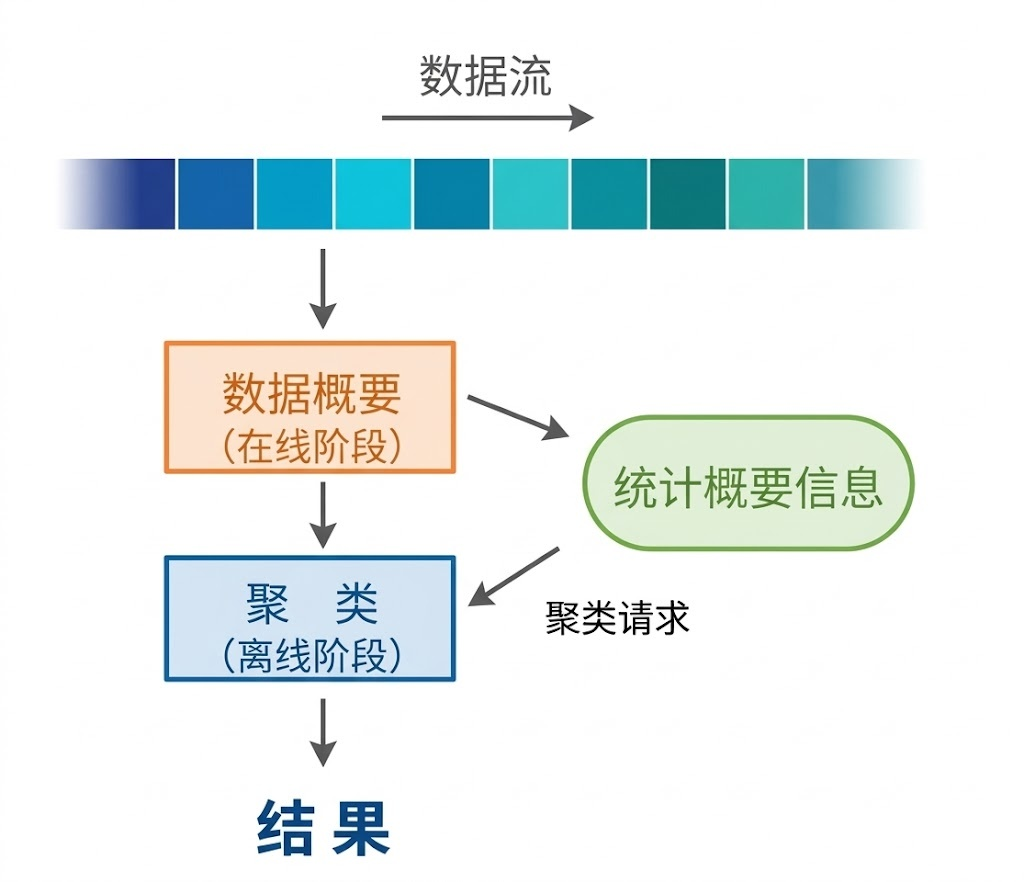
\includegraphics[width=0.65\textwidth]{images/chapter2/two_stage}
	\caption{两阶段在线聚类处理框架图}
	\label{fig:two_stage}
\end{figure}

这类方法的关键在于微簇。微簇并不保存全部历史样本，而是以簇中心、样本数、离散程度以及时间统计量等信息，对局部数据分布进行紧凑表示。当新样本 $u_m$ 到达时，算法先判断其能否并入某个已有微簇；若能够并入，则更新对应的统计摘要；若不能归入现有微簇，则根据当前内存和簇容量约束创建新的微簇，或对旧摘要结构进行合并、替换与压缩。离线阶段再以这些微簇为输入，执行 $k$-means 等宏聚类操作，从而得到用户所需时间范围内的聚类结果。CluStream 体现了这种在线压缩、离线生成的基本思路，而 DenStream\cite{cao2006denstream} 则在此基础上进一步引入潜在微簇、离群微簇和衰减机制，以增强对噪声样本和分布演化的适应能力。总体来看，两阶段方法的优势在于可扩展性较好、在线开销较低；其局限在于最终结果仍依赖额外的离线处理，因此难以持续给出当前时刻的即时聚类结果。

\subsection{完全在线聚类算法}

完全在线聚类算法要求系统在新样本到达后立即完成归类判断，并同步更新簇状态，因此在任意时刻都能够给出当前可用的聚类结果。与先进行在线摘要、再通过离线过程恢复全局簇结构的两阶段方法相比，该类方法更强调结果的即时可用性以及对簇生命周期的持续维护能力，更适用于实时性要求较高的数据流场景。

在代表性的完全在线聚类方法中，CEDAS\cite{hyde2017cedas} 并不直接在原始样本层面维护全局聚类结果，而是先采用固定半径的局部微簇对数据空间进行在线刻画，再通过微簇之间的连接关系描述更高层次的结构演化。具体而言，CEDAS 将连续到达的样本逐步归并到若干微簇中，每个微簇记录其中心位置、支持度以及活跃状态等信息，用以表征数据流在局部区域上的聚集特征。在此基础上，若两个微簇中心分别为 $\boldsymbol{\zeta}_p$ 和 $\boldsymbol{\zeta}_q$，并满足：
\begin{equation}
	\left\|
	\boldsymbol{\zeta}_p-\boldsymbol{\zeta}_q
	\right\|
	\le
	\frac{3}{2}r_0
\end{equation}
则可认为这两个微簇在结构上相邻，并在二者之间建立连接关系。其中，$r_0$ 表示微簇半径。由此，CEDAS 不仅能够利用微簇对局部样本分布进行压缩表示，还能够借助簇间连边刻画数据流聚类结构的整体组织形态。

图\ref{fig:cedas_graph} 给出了 CEDAS 微簇与图结构的示意。左图展示了样本点被多个局部微簇覆盖后的空间分布形式，不同微簇分别对应数据流中的局部聚集区域；右图则进一步给出了依据微簇邻接关系构造得到的图结构。可以看出，CEDAS 所维护的并不是一组彼此孤立的簇中心，而是一个随数据流持续演化的微簇网络。这样的表示方式为后续的在线归并、结构更新和陈旧簇淘汰提供了统一的组织基础。

\begin{figure}[htbp]
	\centering
	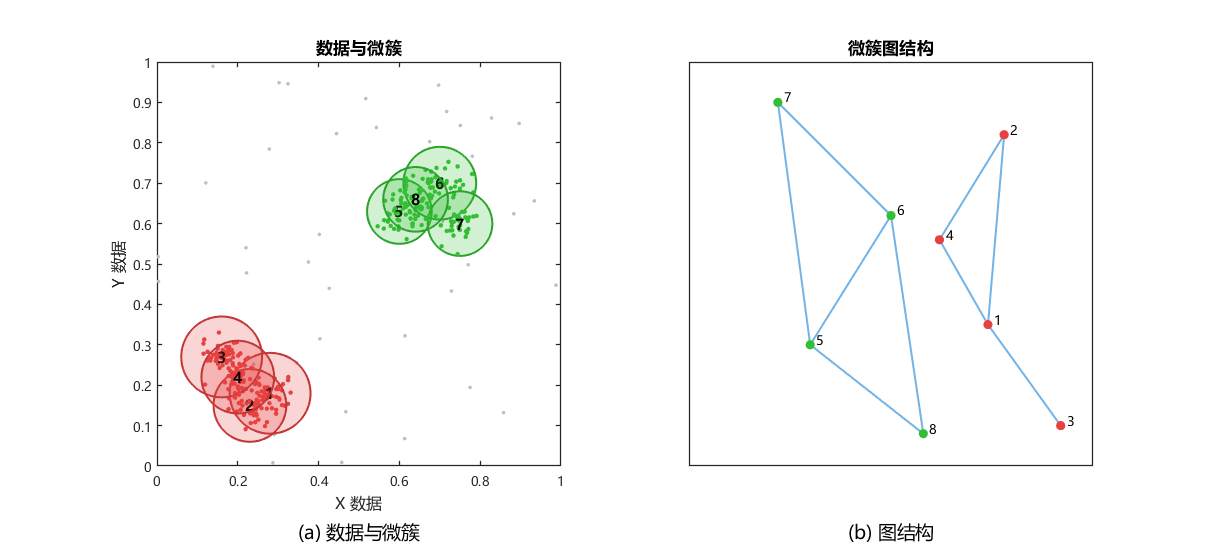
\includegraphics[width=0.85\textwidth]{images/chapter2/CEDAS}
	\caption{CEDAS微簇与图结构示意图}
	\label{fig:cedas_graph}
\end{figure}

在明确了 CEDAS 以微簇与图结构为基本组织方式之后，其在线处理流程便可进一步表述如下。设处理第 $m$ 个样本前的当前微簇集合为：
\begin{equation}
	\mathcal{C}_{m-1}
	=
	\left\{
	C_{m-1}^{(1)},C_{m-1}^{(2)},\ldots,C_{m-1}^{(K_{m-1})}
	\right\}
\end{equation}
其中，$K_{m-1}$ 为当前微簇数，$C_{m-1}^{(c)}$ 表示第 $c$ 个微簇。记第 $c$ 个微簇的中心为 $\boldsymbol{\zeta}_{m-1}^{(c)}$，对于新到达样本 $u_m$，算法首先计算其与各微簇中心之间的距离，并确定最近微簇：
\begin{equation}
	c^{\ast}
	=
	\arg\min_{1\le c\le K_{m-1}}
	d\!\left(u_m,\boldsymbol{\zeta}_{m-1}^{(c)}\right)
\end{equation}
其中，$d(\cdot,\cdot)$ 表示距离度量。

若：
\begin{equation}
	d\!\left(u_m,\boldsymbol{\zeta}_{m-1}^{(c^{\ast})}\right)\le r_0
\end{equation}
则将样本 $u_m$ 并入微簇 $C_{m-1}^{(c^{\ast})}$，并同步更新该微簇的中心、支持度以及相关统计量；否则，说明当前样本无法被已有微簇有效覆盖，此时以 $u_m$ 为中心创建新的微簇。样本归并或建簇完成后，算法还需要依据前述邻接判据更新受影响微簇之间的结构连接关系，从而保证图结构能够及时反映当前数据流的局部组织形态。

除归并与建簇外，CEDAS 还引入了面向数据流场景的生命周期管理机制。随着时间推进，已有微簇的活跃度会持续衰减；对于长期未获得新样本支持的微簇，算法将根据其状态执行失活或删除处理，以避免大量陈旧微簇持续占用存储与计算资源。因而，CEDAS 的核心并不只是样本属于哪个簇的即时判定，更重要的是在持续到达的数据流中同步维护微簇集合、邻接结构及其活跃状态。其整体处理流程如图\ref{fig:cedas_flow} 所示。

\begin{figure}[htbp]
	\centering
	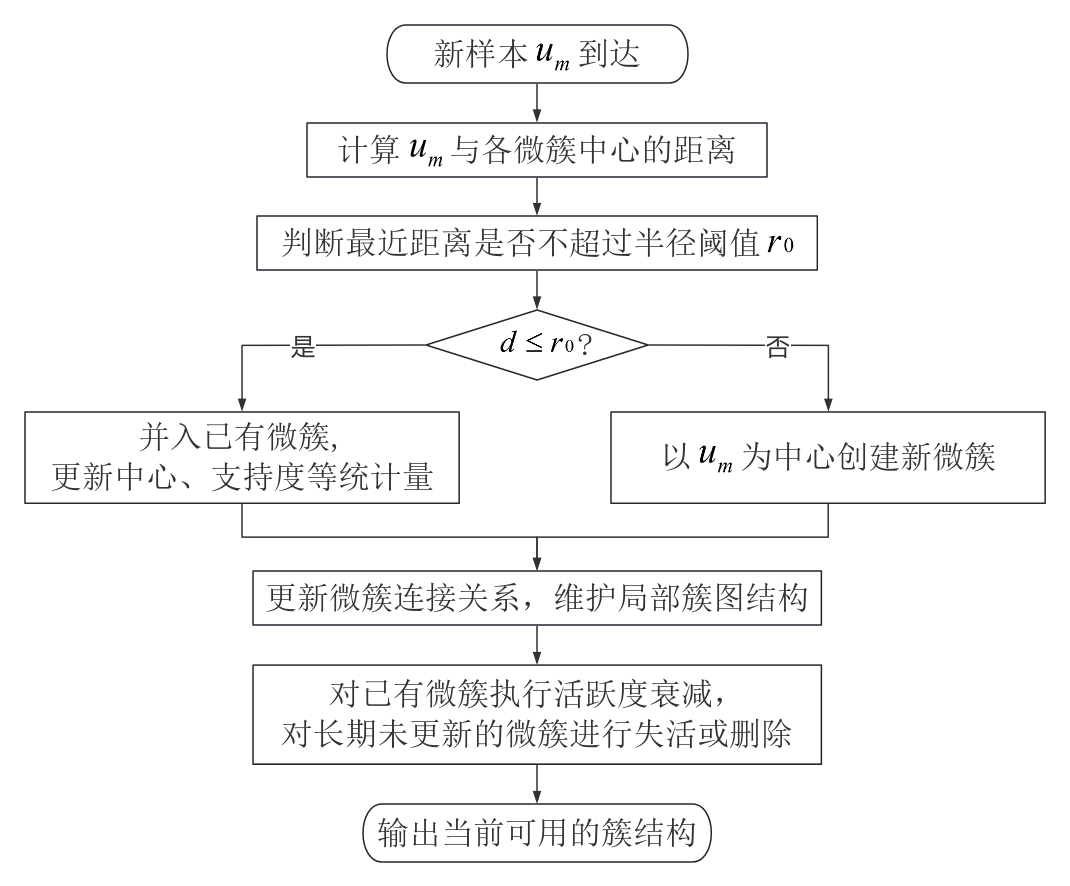
\includegraphics[width=0.72\textwidth]{images/chapter2/CEDAS_flow}
	\caption{CEDAS在线聚类基本流程图}
	\label{fig:cedas_flow}
\end{figure}

相较于两阶段方法，完全在线聚类方法更强调结果的即时可用性以及簇生命周期的持续维护能力。对于本文所面对的地磁检测数据流场景，后台处理端需要随着数据到达持续维护簇结构和中间结果，难以依赖额外的离线重聚类过程，因此其处理需求更接近完全在线聚类框架。也正因如此，后续章节在设计面向长缺测工况的轨迹重构方法时，将更加关注在线归并、结构更新与生命周期管理等机制。


\section{本章小结}
本章对多地磁传感器车辆目标跟踪涉及的基础理论进行了系统梳理。首先从车辆通过传感器时引起的地磁扰动入手，说明了地磁车辆检测的基本机理和检测结果的形成过程；随后介绍了卡尔曼滤波的基本递推过程与目标运动模型，并对常用数据关联方法和在线聚类方法进行了概述。上述内容为后续章节开展在线跟踪算法设计以及长缺测条件下的轨迹片段重构研究提供了必要的理论支撑。


\chapter{非理想量测条件下的多地磁传感器车辆目标跟踪算法}
\label{chap:online_tracking}

\section{引言}

在单向双车道高速公路路段内，多地磁传感器车辆目标跟踪系统实际接收到的检测数据并不总是理想、完整且严格有序的。受无线传输时延、个别地磁传感器短时异常、小型车辆磁扰动较弱以及环境噪声等因素影响，后台量测会出现随机延迟到达、少量漏检和虚警。与此同时，双车道场景下车辆运行关系复杂，邻道干扰与双车长距离并行通过在时空特性上往往十分接近，难以仅凭单条量测直接判断其来源和所属车道。上述因素相互叠加，会同时增加车辆目标跟踪准确跟踪的难度。针对这些问题，本章面向系统常态工况下的非理想量测条件，提出一种基于地磁传感器状态自适应与场景概率判别的多车辆目标跟踪方法，以提高复杂工况下车辆跟踪的准确性、连续性和稳定性。 

围绕这一目标，本章按照先整理量测、再完成跟踪的思路展开。首先，给出系统架构、双车道部署方式和量测模型，并结合理想与非理想数据流的差异，说明漏检、虚警、邻道干扰和量测迟到到达引起的乱序对后续处理的影响。随后，利用时间窗口缓存重排到达顺序，并通过固定滞后窗口接纳迟到量测，在必要时对近期结果局部回放，尽量恢复量测的时间一致性。完成量测整理后，再建立车辆运动模型和量测模型，依次完成状态初始化、状态预测和量测更新，形成连续递推的车辆运动状态估计。在此基础上，针对多车辆并发条件下的量测归属问题，先利用跟踪门缩小候选范围，再通过标准化关联似然和跟踪门内局部关联权重衡量轨迹与量测之间的匹配程度，并结合地磁传感器检测概率和杂波强度的在线估计，使关联判断能够随地磁传感器工作状态和局部杂波水平的变化自适应调整。对于容易混淆的邻道干扰与真实双车并行，进一步构建三状态场景递推判别模型，将局部交通场景区分为左车道真实车辆伴随右侧干扰、右车道真实车辆伴随左侧干扰以及两车道真实车辆并行通过三种情况，为量测归属和车道判断提供连续依据。最后，在轨迹管理阶段，结合目标存在概率递推与基于场景后验的车道状态更新机制，完成轨迹的起始、确认、维持、删除以及车道状态修正，形成完整的在线跟踪流程，并通过仿真与实验对各关键环节及整体性能进行验证。

\section{双车道多地磁传感器系统架构与建模}\label{sec:ch2_platform}

相比单个地磁传感器，多地磁传感器协同检测具有更好的可靠性和覆盖能力。沿道路连续布设多个地磁传感器后，车辆在不同观测位置的通过信息可以被依次记录；即使个别地磁传感器受干扰影响而暂时失效，其余地磁传感器的检测数据仍可支撑系统正常运行。与此同时，车辆在某一检测时刻的位置可近似视为对应地磁传感器的预设安装位置，因此联合多地磁传感器检测数据能够为车辆运动状态估计提供更充分的时空约束。为开展后续车辆目标跟踪研究，下面分别介绍系统架构、地磁传感器部署模型及量测模型。
\subsection{系统架构概述}

本文搭建了由地磁传感器、数据传输模块、后台处理模块和平台展示模块组成的多地磁车辆感知系统，其总体结构如图~\ref{fig:ch2_system_architecture}所示。系统前端负责车辆检测数据采集，中间层负责多地磁传感器数据汇聚与回传，后台负责数据接入、处理以及车辆目标跟踪结果输出，平台展示模块负责对跟踪结果进行可视化展示。

\begin{figure}[H]
	\centering
	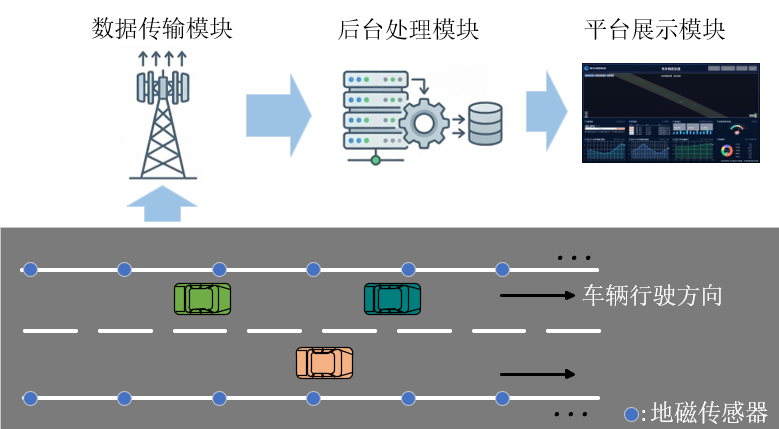
\includegraphics[width=0.77\textwidth]{images/chapter2/fig_2_5_system_v1.png}
	\caption{多地磁传感器车辆目标跟踪系统架构示意图}
	\label{fig:ch2_system_architecture}
\end{figure}

首先，前端地磁传感器负责连续采集路面附近的磁场变化并检测车辆通过。本系统采用一体化地磁传感器设计，将三轴地磁传感器 VCM5883、微控制器（Microcontroller Unit，MCU）、LoRa通信模块以及太阳能供电与充电单元集成在同一设备中，实物如图~\ref{fig:ch2_geomagnetic_sensor_real}所示。VCM5883 持续输出三轴磁场数据，MCU 在端侧完成必要的预处理、阈值判别和状态机检测，并在车辆通过后生成检测数据。单条检测数据通常包含车辆经过对应地磁传感器编号、地磁传感器的触发时间、所在位置以及车辆所引起的磁场扰动峰值等字段。生成后的检测数据经 LoRa 通信模块上传至数据传输模块；太阳能供电与充电单元则用于保障地磁传感器在无外接电源条件下的长期稳定运行。
\begin{figure}[H]
	\centering
	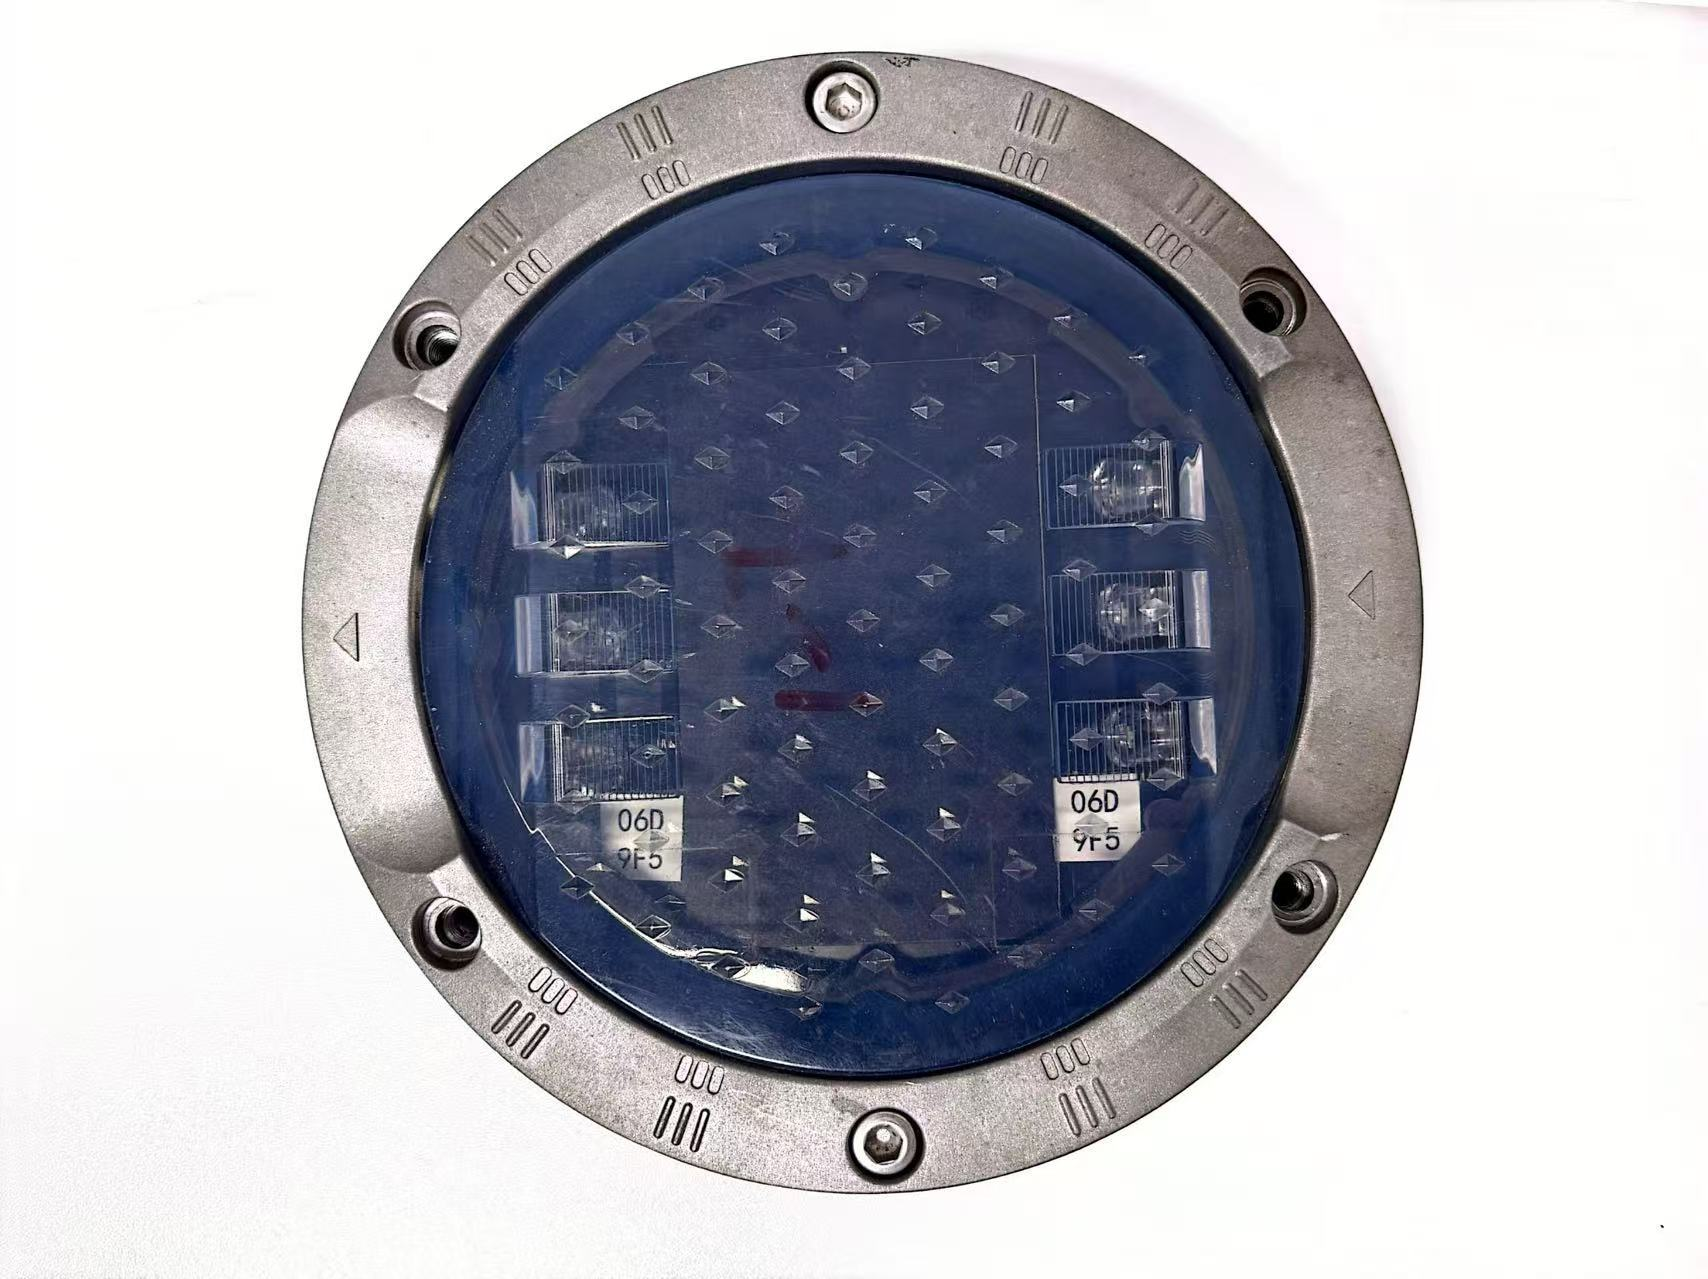
\includegraphics[width=0.40\textwidth]{images/chapter2/fig_2_4_geomagnetic_sensor}
	\caption{地磁传感器实物图}
	\label{fig:ch2_geomagnetic_sensor_real}
\end{figure}
其次，数据传输模块负责多地磁传感器检测数据的汇聚与回传，其实物如图~\ref{fig:ch2_comm_base_real}所示。该模块一方面可通过 LoRa 与沿线部署的多个地磁传感器建立无线通信，接收并缓存各地磁传感器上传的检测数据；另一方面可通过 4G 网络按预设时间间隔将检测数据打包发送至后台处理模块，从而实现前端检测数据的集中回传。考虑到实际道路环境中的通信条件变化，LoRa 的有效通信距离一般为 3$\sim$5 km。需要说明的是，检测数据流在后台侧按到达顺序进入处理链路，受无线链路时延与回传机制影响，部分量测可能出现随机延迟甚至迟到到达，导致数据到达顺序与实际触发时间顺序不一致，从而对后续关联与更新产生直接影响。
\begin{figure}[H]
	\centering
	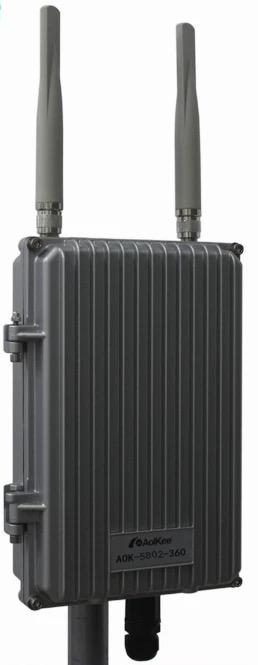
\includegraphics[width=0.15\textwidth]{images/chapter2/fig_2_1_base}
	\caption{数据传输模块实物图}
	\label{fig:ch2_comm_base_real}
\end{figure}
再次，后台处理模块负责对上传的地磁传感器检测数据进行统一接入与在线处理，本文以云服务器作为后台载体。后台持续接收数据传输模块回传的地磁传感器检测数据，首先完成数据解析、校验和量测时序整理；随后结合量测时序矫正、数据关联、状态估计、邻道干扰与双车并行场景判别以及车道状态更新，对同一车辆在不同观测位置形成的离散量测进行联合处理，逐步估计车辆在监测路段内的位置、速度和所属车道，输出连续的车辆目标跟踪结果。当连续漏检累积并造成轨迹明显断裂时，后台不再回到原始地磁传感器检测数据上重复执行点级跟踪，而是以前一阶段得到的轨迹片段和少量未关联量测为输入，采用基于在线聚类的轨迹片段重构方法，对彼此衔接的断裂片段进行聚类、匹配与拼接，以恢复更完整的车辆轨迹。其中涉及的量测时序矫正、关联建模、状态递推、轨迹管理和在线聚类重构等算法，也是本文后续章节重点研究的内容。

最后，平台展示模块负责对后台输出的车辆目标跟踪结果进行实时展示。后台处理模块完成车辆实时位置计算后，将车辆位置、所属车道及相关运行信息推送至平台端界面，平台据此对路段内车辆运行状态和系统工作状态进行可视化展示。本文搭建的前端展示界面如图~\ref{fig:ch2_online_platform}所示。
\begin{figure}[H]
	\centering
	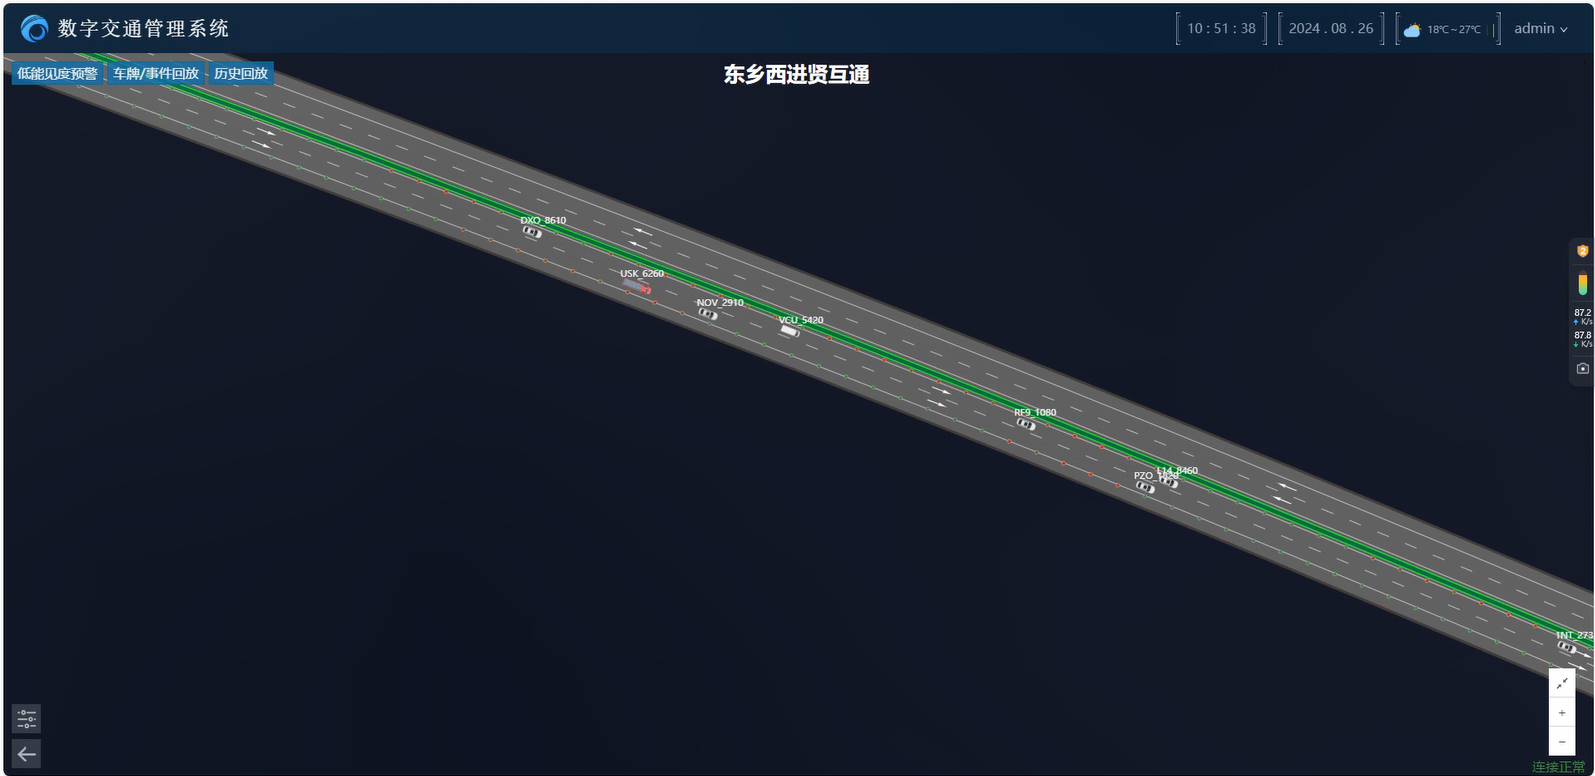
\includegraphics[width=0.85\textwidth]{images/chapter2/fig_2_7_platform}
	\caption{车辆目标跟踪前端展示界面}
	\label{fig:ch2_online_platform}
\end{figure}

\subsection{双车道多地磁传感器部署模型}\label{sec:ch2_summary}

图~\ref{fig:ch2_road_layout}给出了本文研究的单向双车道场景及地磁传感器部署方式。为获得可用于车辆目标跟踪的离散量测序列，本文沿车辆行驶方向以固定间距设置多个观测位置；在每个观测位置的两侧边界车道线附近各部署一个地磁传感器，从而形成左右成对的观测点。图中实心圆点表示地磁传感器。车辆沿道路行驶时，会依次在不同观测位置形成检测记录，这为后续速度估计、数据关联和轨迹构建提供了基础输入。
\begin{figure}[H]
	\centering
	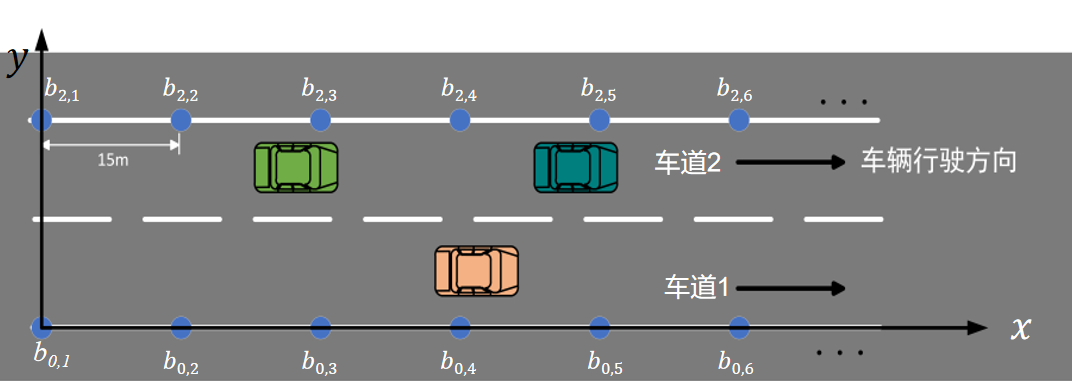
\includegraphics[width=0.85\textwidth]{images/chapter2/fig_2_8_roadv2}
	\caption{单向双车道场景地磁传感器部署示意图}
	\label{fig:ch2_road_layout}
\end{figure}
为便于后续建模与推导，建立道路坐标系：以车辆行驶方向为 $x$ 轴正方向，以纵向跨车道方向为 $y$ 轴正方向，并取上游第一组地磁传感器所在的观测位置为坐标原点。本文仅考虑在两条边界车道线附近布设地磁传感器，并与后续车道线索引保持一致，将两条布设车道线编号为：
\begin{equation}
	l \in \{0,2\},
	\label{eq:ch2_lane_index}
\end{equation}

其中，$l=0$ 表示沿车辆行驶方向最右侧边界车道线，$l=2$ 表示最左侧边界车道线。沿行驶方向的地磁传感器按组编号记为：
\begin{equation}
	r=0,1,\ldots,N_{\mathrm{grp}}-1,
	\label{eq:ch2_group_index}
\end{equation}
其中，$N_{\mathrm{grp}}$ 表示沿车辆行驶方向布设的地磁传感器组数。则位于车道线 $l$ 且属于第 $r$ 组的地磁传感器记为 $b_{l,r}$。进一步地，记 $r(j)$ 为量测 $\mathbf z_j$ 所属的观测位置组编号。若触发地磁传感器满足 $b_j=b_{l,r}$，则有 $r(j)=r$。地磁传感器的空间位置用二维坐标向量表示为：
\begin{equation}
	\mathbf{s}_{l,r} =
	\begin{bmatrix}
		x_r \\
		y_l
	\end{bmatrix},
	\qquad
	l\in\{0,2\},\; r=0,1,\ldots,N_{\mathrm{grp}}-1,
	\label{eq:ch2_sensor_position}
\end{equation}
其中，$x_r$ 为第 $r$ 个横向观测位置的坐标，$y_l$ 为对应边界车道线的纵向坐标。本文采用对称布设方式，即同一组中的 $b_{0,r}$ 与 $b_{2,r}$ 位于同一横向观测位置，二者具有相同的 $x_r$，仅在横向位置 $y$ 上不同。相邻两组观测位置的横向间距记为 $L_a$，则有：
\begin{equation}
	x_r = x_0 + rL_a,
	\qquad r=0,1,\ldots,N_{\mathrm{grp}}-1,
	\label{eq:ch2_sensor_spacing}
\end{equation}
其中，$x_0$ 为第一组观测位置的横向坐标，后续推导中通常取 $x_0=0$ 以简化表达。

需要指出的是，对称布设在工程实现与空间标定上较为直接，但在双车道并行行驶或换道条件下也会提高数据关联难度：一方面，同一横向观测位置同时存在左右两个观测点，不同车辆的检测时间可能相互接近甚至部分重叠；另一方面，车辆沿$y$轴位置变化会使左右地磁传感器的触发时间和扰动强度产生偏移，因此仅依据时空邻近关系往往难以稳定完成对应匹配。基于上述部署模型，下一节将给出量测的统一表示，并结合理想与非理想检测数据流说明后续跟踪中面临的主要不确定性。

\subsection{双车道多地磁传感器量测模型}

当地磁传感器检测到车辆通过后，系统会向后台上传一条检测数据。将后台按到达顺序接收的第 $j$ 条检测数据记为量测向量 $\mathbf z_j$，结合本文系统的上报格式，量测可定义为：
\begin{equation}
	\mathbf z_j=
	\begin{bmatrix}
		t_j &
		b_j &
		x_{b_j} &
		y_{b_j} &
		l_j &
		Mpeak_j
	\end{bmatrix}^{\mathrm T},
	\label{eq:ch2_measurement_vector}
\end{equation}
其中，$t_j$ 为触发时间戳，$x_{b_j}$ 和 $y_{b_j}$ 分别为该触发地磁传感器在道路坐标系下的横向和纵向安装坐标，$l_j$ 为该设备所属边界车道线编号，$Mpeak_j$ 为对应车辆引起的磁场扰动峰值。式~\eqref{eq:ch2_measurement_vector}描述了车辆在时刻 $t_j$ 于观测点 $(x_{b_j},y_{b_j})$ 附近形成的一次离散量测。


(1) 理想检测数据流形态

图~\ref{fig:ch2_detection_flow}(a)给出了理想情况下检测数据流的典型形态。图中以时间戳 $t$ 为横轴，以道路横向位置 $x$ 为竖轴，斜向坐标表示边界车道线编号 $l$，每一个散点对应一条检测记录，连线仅用于表示同一车辆的连续通过过程。

\begin{figure}[H]
	\centering
	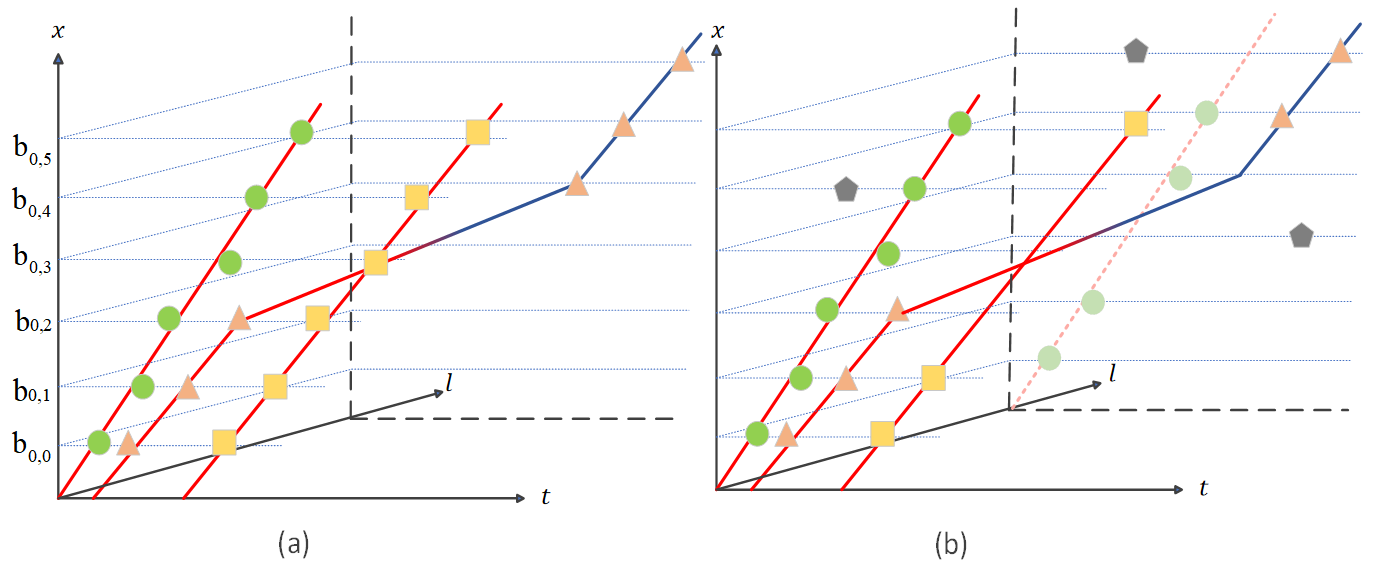
\includegraphics[width=0.88\textwidth]{images/chapter2/fig_2_9_data_v3}
	\caption{地磁传感器检测数据在理想与非理想情况下的分布示意图}
	\label{fig:ch2_detection_flow}
\end{figure}

如图所示，绿色圆点和黄色方块分别表示两辆始终在各自车道内直行的车辆，它们的检测记录沿对应车道线随时间依次向下游推进，在图中形成两条连续、平滑的直行轨迹。橙色三角形表示另一辆发生换道的车辆，其检测记录在纵向持续向前推进的同时，在车道线维上由一侧逐步过渡到另一侧，因此形成一条具有明显横向转移特征的换道轨迹。可以看出，在理想条件下，同一车辆的检测记录在时间顺序、纵向推进和车道归属上都具有较强连续性，这为后续的数据关联和状态估计提供了清晰的先验结构。

(2) 非理想检测数据流形态

真实道路环境下，检测数据流通常表现为图~\ref{fig:ch2_detection_flow}(b)中的所示形态。与理想情况相比，原本连续的轨迹结构会受到多种不确定因素干扰。

首先是漏检导致的量测缺失。部分观测位置未形成有效检测记录，既可能表现为单次缺失，如橙色三角形轨迹所示；也可能在若干相邻观测位置上连续缺失，如黄色方块轨迹所示，这些量测的缺失可能使同一车辆的量测点出现明显空档并导致轨迹结构断裂。这会直接削弱由时间差推得的速度约束，并增大后续关联的不确定性。

其次是是虚警导致的离散杂波量测。环境噪声或异常电磁扰动可能产生与真实车辆无关的检测点，如图中灰色五边形量测点所示，这类量测通常分布较为离散，且缺乏与真实车辆一致的时空连续性。当车流密度较高时，这类离散杂波量测会显著扩大候选关联集合，增加误关联风险。

再次邻道干扰导致的伪轨迹量测。在双车道场景中，相邻车道车辆尤其是大型车辆通过时，由于其铁磁材料较多且磁扰动范围更大，另一侧地磁传感器也可能被同步或连续触发。图~\ref{fig:ch2_detection_flow}中的浅绿色圆点即表示此类由真实车辆诱发的干扰量测。需要指出的是，这些量测并不对应另一侧的一辆独立真实车辆，但在若干相邻观测位置上仍可能沿车辆行驶方向形成近似连续的时空结构，从而表现出与真实单车通过相似的伪轨迹形态。进一步地，当道路上确有两辆车长时间并行通过时，两侧量测在时间差、横向推进顺序上又会与上述邻道干扰情形较为接近，因此仅依据单次触发或局部量测形态往往难以直接区分。

最后是随机传输时延导致的量测迟到与乱序到达。对于同一车辆，各观测位置形成的检测量测在物理触发顺序上通常是有序的；然而受无线链路传输时延等因素的影响，量测到达算法模块的先后顺序可能与其实际触发顺序不一致，从而出现迟到到达甚至局部乱序。当某条本应在当前时刻参与关联的量测尚未到达时，轨迹只能依据当下已接收的数据进行更新，此时就可能错误关联到其他车辆的量测而导致状态估计发生漂移，也可能暂时未能获得正确关联，转而在后续时刻与该车辆之后到来的量测建立匹配，这样一来，先前迟到的那条量测在随后进入系统时，往往已经错过其最合适的关联时机，进而可能继续干扰其他车辆的量测分配，诱发连锁性的误关联。

因此，本文所研究的多地磁传感器车辆目标跟踪问题，本质上是在存在漏检、邻道干扰、离散杂波以及随机时延导致的迟到与乱序量测等不确定因素的条件下，利用多点检测数据完成车辆量测关联，并进一步估计车辆的运动状态与行驶车道。后续章节将在此基础上展开具体算法设计，并重点处理邻道干扰与真实双车并行等易混淆场景的判别问题。




\section{量测时序矫正}

在量测进入状态估计与数据关联模块之前，有必要首先对其进行时序矫正，在有限滞后范围内尽可能恢复量测的真实触发顺序，从而为后续跨地磁传感器关联提供时间一致且信息尽可能完整的输入。

\subsection{基于时间窗口缓存的量测时序重排}

时间窗口缓存本质上就是按扫描序号组织的量测集合序列，系统在线处理时按该序列维护各扫描槽位，从而既保留了时间先后关系，也为迟到量测回插预留了位置。

给定参考时刻 $t_0$，事件 $\mathbf z_j$ 所属的扫描序号定义为：
\begin{equation}
	n(j)=\left\lfloor \frac{t_j-t_0}{\Delta T} \right\rfloor +1
	\label{eq:ch3_scan_index}
\end{equation}
其中，$\Delta T$ 为时间窗口缓存的扫描时间片长度，其取值通常结合系统允许的处理时延、输出刷新要求以及迟到量测延迟分布的统计结果共同设定。于是，第 $n$ 个扫描内的量测集合可写为：
\begin{equation}
	\mathcal Z_n=
	\left\{
	\mathbf z_j\,\big|\, n(j)=n
	\right\}
	\label{eq:ch3_scan_set}
\end{equation}
时间窗口缓存本质上就是按扫描序号排列的若干个量测集合，系统在线处理时只维护其中最近一段时间内的扫描时间片，从而既保留了时间先后关系，也为迟到量测回插预留了位置。

同一扫描内，不同地磁传感器上报的量测到达顺序可能与真实触发顺序不一致，因此还需要在扫描内部按触发时间戳升序排序，得到：
\begin{equation}
	\mathcal Z_n^{\uparrow}=\mathrm{Sort}\left(\mathcal Z_n; t_j\uparrow\right)
	\label{eq:ch3_scan_sort}
\end{equation}
后续的状态预测、量测关联和轨迹更新均按照 $\mathcal Z_n^{\uparrow}$ 中的顺序逐条执行。这样，系统先在扫描层面对事件作粗粒度对齐，再在扫描内部恢复真实先后关系，使进入后续递推的事件流在时间上尽可能一致。

\subsection{基于固定滞后窗口的局部处理结果回退}

扫描内排序可以解决同一扫描中的局部乱序，但仍不能处理跨扫描迟到到达的量测。为此，在时间窗口缓存上进一步引入固定滞后窗口，以当前第$n$个扫描为右端点对最近 $L$ 个扫描保持可回溯状态。以当前扫描序号 $n$ 为右端点的活动窗口定义为：
\begin{equation}
	\mathcal W_n=
	\left\{
	\mathcal Z_{n-L+1},\ldots,\mathcal Z_n
	\right\}
	\label{eq:ch3_lag_window}
\end{equation}
同时，在窗口左端保留快照状态：
\begin{equation}
	\mathcal S_{n-L}=
	\left\{
	\hat{\mathbf x}_{i,k|k},\mathbf P_{i,k|k},P_{E,i},
	\boldsymbol\pi_i^{\mathrm{lane}},
	\boldsymbol\pi_r^{\mathrm{scene}},
	\alpha_{D,b},\beta_{D,b},a_{\lambda_c,b},b_{\lambda_c,b}
	\right\}
	\label{eq:ch3_snapshot_reorg}
\end{equation}
其中，$k=n-L$ 表示窗口左端之前最近一次已提交扫描对应的时刻；$\hat{\mathbf x}_{i,k|k}$ 和 $\mathbf P_{i,k|k}$ 分别为轨迹 $i$ 在该时刻的后验状态估计与协方差，$P_{E,i}$ 为轨迹存在概率，$\boldsymbol\pi_i^{\mathrm{lane}}$ 为轨迹 $i$ 的车道后验向量，$\boldsymbol\pi_r^{\mathrm{scene}}$ 为第 $r$ 组观测位置对应的左右地磁传感器对的场景后验向量，其中 $r=0,1,\ldots,N_{\mathrm{grp}}-1$；$\alpha_{D,b}$ 与 $\beta_{D,b}$ 为地磁传感器 $b$ 检测概率的 Beta 后验参数，$a_{\lambda_c,b}$ 与 $b_{\lambda_c,b}$ 为地磁传感器 $b$ 杂波空间密度的 Gamma 后验参数，这些参数的计算与更新将在后续给出。另外注意，所称已提交是指该扫描已经不再参与后续局部回放，其关联、状态更新和轨迹管理结果被视为当前在线流程中的确定历史。之所以需要同时保留这些信息，是因为局部回放不仅要回退轨迹运动状态，还要恢复当时用于关联、场景判别和地磁传感器状态更新的先验条件，这样重新执行窗口内各扫描时，才能与原始处理链条保持一致。

当新到达量测 $\mathbf z_j$ 满足
\begin{equation}
	n(j)\in\{n-L+1,\ldots,n\},
	\label{eq:ch3_late_condition}
\end{equation}
则认为其属于固定滞后窗口内的迟到量测。此时，系统先将该量测回插至对应历史扫描的量测集合中，再从快照 $\mathcal S_{n-L}$ 出发，将该快照之后已经生成的关联、状态更新和轨迹管理结果全部回退，并按时间顺序重新执行窗口内的状态预测、场景判别、数据关联、量测更新和轨迹管理流程。若量测所属扫描早于窗口左端，则说明其已超出当前在线可修正范围，不再纳入跟踪流程。借助固定滞后窗口与局部回放机制，系统可以利用后续到达的信息对近期历史关联结果进行局部修正，在不过度增加计算开销的前提下，改善短时乱序和迟到条件下的轨迹连续性与结果一致性。

\section{基于多地磁传感器数据的车辆运动状态估计算法}
\label{sec:ch3_state_estimation}

完成量测时序矫正后，系统获得了按真实触发时间组织的地磁传感器数据流输入。接下来需要在此基础上建立与地磁事件流相匹配的车辆状态估计算法，把车辆在某一时刻通过某一已知地磁传感器的离散检测事实转化为可递推的状态约束，为后续的数据关联、场景判别和轨迹管理提供统一的状态表达。


\subsection{车辆运动模型与观测模型}

由于双车道地磁系统并不直接提供车辆纵向连续坐标，本文仅对车辆沿$x$轴行驶方向的连续状态进行递推估计，而将地磁传感器纵向安装位置、边界车道线编号和地磁扰动峰值等信息作为离散证据保留，用于后续的数据关联与车道状态判别。考虑到车辆在高速路段沿车道横向行驶，且相邻地磁传感器之间的通过时间通常处于较短时间尺度内，本文采用常速度（CV）模型作为车辆沿$x$轴方向的运动基础模型。设轨迹 $i$ 在第 $k$ 次有效更新后的状态向量为：
\begin{equation}
	\mathbf x_{i,k}=
	\begin{bmatrix}
		p_{i,k}\\
		v_{i,k}
	\end{bmatrix},
	\label{eq:ch3_state_vec}
\end{equation}
其中，$p_{i,k}$ 与 $v_{i,k}$ 分别表示车辆在道路横向上的位置与速度。

若轨迹 $i$ 在相邻两次有效更新之间的时间间隔为 $\Delta t_{i,k+1}$，则其状态转移模型写为：
\begin{equation}
	\mathbf x_{i,k+1}=
	\mathbf F\left(\Delta t_{i,k+1}\right)\mathbf x_{i,k}+\mathbf w_{i,k},
	\label{eq:ch3_state_transition}
\end{equation}
其中，状态转移矩阵为：
\begin{equation}
	\mathbf F\left(\Delta t_{i,k+1}\right)=
	\begin{bmatrix}
		1 & \Delta t_{i,k+1}\\
		0 & 1
	\end{bmatrix},
	\label{eq:ch3_F}
\end{equation}
过程噪声满足 $\mathbf w_{i,k}\sim\mathcal N(\mathbf 0,\mathbf Q(\Delta t_{i,k+1}))$。考虑短时机动和时间戳抖动对横向传播误差的影响，过程噪声协方差写为：
\begin{equation}
	\mathbf Q\left(\Delta t_{i,k+1}\right)
	=
	q_a
	\begin{bmatrix}
		\dfrac{\Delta t_{i,k+1}^{4}}{4} & \dfrac{\Delta t_{i,k+1}^{3}}{2}\\[6pt]
		\dfrac{\Delta t_{i,k+1}^{3}}{2} & \Delta t_{i,k+1}^{2}
	\end{bmatrix}
	+
	\begin{bmatrix}
		c_t \hat v_{i,k+1|k}^{\,2}\sigma_t^2 & 0\\
		0 & 0
	\end{bmatrix}
	\label{eq:ch3_Q}
\end{equation}
当地磁传感器量测最终被关联到轨迹后，说明车辆在时刻 $t_j$ 经过了地磁传感器 $b_j$ 所在的纵向观测位置，因此该量测可进一步转化为对车辆纵向位置的约束。记地磁传感器 $b_j$ 的纵向安装坐标为 $x_{b_j}$，则定义伪位置观测：
\begin{equation}
	\tilde p_{i,k+1}=x_{b_j}
	\label{eq:ch3_pseudo_meas}
\end{equation}
相应的观测模型写为：
\begin{equation}
	\tilde p_{i,k+1}=\mathbf H\mathbf x_{i,k+1}+e_{i,k+1}
\end{equation}
其中，观测矩阵为：
\begin{equation}
	\mathbf H=
	\begin{bmatrix}
		1 & 0
	\end{bmatrix}
\end{equation}
观测噪声项满足：
\begin{equation}
	e_{i,k+1}\sim\mathcal N(0,R_{b_j})
	\label{eq:ch3_measurement_k}
\end{equation}
式中，$R_{b_j}$ 为与地磁传感器 $b_j$ 相关的观测方差。需要说明的是，$R_{b_j}$ 反映的是地磁传感器安装标定误差以及地磁传感器工作状态波动折算到位置约束上的综合不确定性，而非时间戳误差方差。后文将结合地磁传感器检测概率与杂波强度的在线估计结果，对 $R_{b_j}$ 进行自适应调整。

\subsection{状态初始化}

对于当前扫描中尚未与任何已确认轨迹关联的量测，系统将其作为新生轨迹的初始化对象；新生轨迹在完成初始化后，不再参与当前时刻已有轨迹的关联竞争。设事件 $\mathbf z_{j_0}$ 触发了新候选轨迹 $i$，则其初始位置取为对应地磁传感器的横向坐标：
\begin{equation}
	p_{i,0}=x_{b_{j_0}}
	\label{eq:ch3_init_pos}
\end{equation}
由于单条地磁事件无法可靠提供速度信息，本文采用道路历史平均速度或经验速度 $\bar v_0$ 作为初始速度先验，从而得到初始状态均值：
\begin{equation}
	\hat{\mathbf x}_{i,0|0}=
	\begin{bmatrix}
		p_{i,0}\\
		\bar v_0
	\end{bmatrix}
	\label{eq:ch3_init_state}
\end{equation}
对应的初始协方差取为：
\begin{equation}
	\mathbf P_{i,0|0}=\mathrm{diag}\left(\sigma_{p0}^{2},\sigma_{v0}^{2}\right)
	\label{eq:ch3_init_cov}
\end{equation}
其中，$\sigma_{p0}^{2}$ 表示新生轨迹初始纵向位置的先验方差，$\sigma_{v0}^{2}$ 表示新生轨迹初始纵向速度的先验方差。考虑到初始时刻车辆位置可由触发量测对应的地磁传感器纵向安装位置近似给出，$\sigma_{p0}^{2}$ 可取与地磁传感器位置观测方差同量级；而由于初始阶段车辆速度尚缺乏充分观测信息，$\sigma_{v0}^{2}$ 通常取较大的先验值，以反映新生轨迹在初始阶段速度不确定性较高。

为使地磁扰动峰值信息能够进入后续关联计算，本文同时维护轨迹级对数磁峰值统计量。设新生事件的对数峰值为：
\begin{equation}
	m_{i,0}=\log(Mpeak_{j_0}+\varepsilon_M)
	\label{eq:ch3_init_mag}
\end{equation}
则其磁特征均值初始化为：
\begin{equation}
	\mu_{i,0}^{M}=m_{i,0}
	\label{eq:ch3_init_mag_mean}
\end{equation}
对应的磁特征方差初始化为：
\begin{equation}
	(\sigma_{i,0}^{M})^{2}=\sigma_{M0}^{2}
	\label{eq:ch3_init_mag_var}
\end{equation}

这样设置的目的是使新生轨迹在具备位置与速度先验的同时，保留可供后续关联使用的地磁特征先验。

\subsection{状态预测}

设轨迹 $i$ 在第 $k$ 次有效更新后的后验状态均值与协方差分别为 $\hat{\mathbf x}_{i,k|k}$ 和 $\mathbf P_{i,k|k}$。若后续某个量测最终对应其第 $k+1$ 次有效更新，则该事件触发时间记为 $t_j$，相邻两次有效更新之间的时间间隔定义为：
\begin{equation}
	\Delta t_{i,k+1}=t_j-t_{i,k}
	\label{eq:ch3_dt_update}
\end{equation}
于是，轨迹 $i$ 在第 $k+1$ 次更新前的预测状态均值与预测协方差分别为：
\begin{equation}
	\hat{\mathbf x}_{i,k+1|k}
	=
	\mathbf F\left(\Delta t_{i,k+1}\right)\hat{\mathbf x}_{i,k|k}
	\label{eq:ch3_predict_state}
\end{equation}
\begin{equation}
	\mathbf P_{i,k+1|k}
	=
	\mathbf F\left(\Delta t_{i,k+1}\right)
	\mathbf P_{i,k|k}
	\mathbf F^{\mathrm T}\left(\Delta t_{i,k+1}\right)
	+
	\mathbf Q\left(\Delta t_{i,k+1}\right)
	\label{eq:ch3_predict_cov}
\end{equation}
由此可将轨迹状态传播到候选事件触发时刻，为后续量测关联和滤波更新提供统一的预测先验。

\subsection{量测更新}

若轨迹 $i$ 最终被分配到事件 $\mathbf z_j$，则由伪位置观测模型可得新息为：
\begin{equation}
	\nu_{i,k+1}=\tilde p_{i,k+1}-\mathbf H\hat{\mathbf x}_{i,k+1|k}
	\label{eq:ch3_innovation_event}
\end{equation}
对应的新息方差为：
\begin{equation}
	S_{i,k+1}=\mathbf H\mathbf P_{i,k+1|k}\mathbf H^{\mathrm T}+R_{b_j}
	\label{eq:ch3_S_event}
\end{equation}
于是，Kalman 增益写为：
\begin{equation}
	\mathbf K_{i,k+1}
	=
	\mathbf P_{i,k+1|k}\mathbf H^{\mathrm T}
	\left(
	\mathbf H\mathbf P_{i,k+1|k}\mathbf H^{\mathrm T}+R_{b_j}
	\right)^{-1}
	\label{eq:ch3_K_event}
\end{equation}
相应的状态均值与协方差更新为：
\begin{equation}
	\hat{\mathbf x}_{i,k+1|k+1}
	=
	\hat{\mathbf x}_{i,k+1|k}
	+
	\mathbf K_{i,k+1}\nu_{i,k+1}
	\label{eq:ch3_update_state_event}
\end{equation}
\begin{equation}
	\mathbf P_{i,k+1|k+1}
	=
	\left(\mathbf I-\mathbf K_{i,k+1}\mathbf H\right)\mathbf P_{i,k+1|k}
	\label{eq:ch3_update_cov_event}
\end{equation}
若轨迹在当前扫描内未获得有效关联，则不执行量测更新，而仅保留预测结果，并将该次未命中事实作为后续目标存在概率递推和地磁传感器检测概率统计更新的输入证据。至此，本文建立了与地磁传感器数据流相匹配的量测级状态估计框架。下面进一步解决多车辆共享地磁传感器数据流条件下的量测归属与场景消歧问题。

\section{数据关联算法设计}
\label{sec:ch3_association}

在完成车辆状态估计模型之后，下一步需要处理地磁传感器检测数据流中的量测来源不确定性问题。对于双车道地磁系统而言，量测归属不仅取决于时间一致性，还受到地磁传感器检测能力差异、杂波水平变化以及邻道干扰与真实双车并行混淆的共同影响。因此，本节围绕跟踪门、关联似然与跟踪门内局部关联权重、地磁传感器状态自适应以及并行场景判别四个方面构建统一的概率建模框架。


\subsection{车辆目标跟踪门}

由于地磁传感器量测在时间轴上异步到达，系统无法像同步采样传感器那样在单一采样时刻统一判断所有事件的来源。因此，本文首先基于时间一致性构造轨迹关联跟踪门。对任意候选事件 $\mathbf z_j$，记其触发地磁传感器编号为 $b_j$，对应地磁传感器的横向安装坐标为 $x_{b_j}$，触发时间戳为 $t_j$。若轨迹 $i$ 在当前状态下可能继续前进至该地磁传感器，则由常速度模型可得到其预测通过地磁传感器 $b_j$ 的时刻：
\begin{equation}
	\hat t_{i\rightarrow b_j}
	=
	t_{i,k}+\frac{x_{b_j}-\hat p_{i,k|k}}{\hat v_{i,k|k}}
	\label{eq:ch3_pred_time}
\end{equation}
于是，事件 $\mathbf z_j$ 与轨迹 $i$ 之间的时间残差定义为：
\begin{equation}
	\nu^{t}_{i,j}=t_j-\hat t_{i\rightarrow b_j}
	\label{eq:ch3_time_residual}
\end{equation}
由式~\eqref{eq:ch3_pred_time} 对状态变量 $(p,v)$ 作一阶线性化，可得雅可比向量：
\begin{equation}
	\mathbf J_{i,j}
	=
	\begin{bmatrix}
		-\dfrac{1}{\hat v_{i,k|k}} & -\dfrac{x_{b_j}-\hat p_{i,k|k}}{\hat v_{i,k|k}^{\,2}}
	\end{bmatrix}
	\label{eq:ch3_time_jacobian}
\end{equation}
从而时间残差方差写为：
\begin{equation}
	S^{t}_{i,j}=\mathbf J_{i,j}\mathbf P_{i,k|k}\mathbf J_{i,j}^{\mathrm T}+\sigma_{t,b_j}^{2}
	\label{eq:ch3_time_var}
\end{equation}
其中，$\sigma_{t,b_j}^{2}$ 表示地磁传感器 $b_j$ 的时间戳误差方差。基于此，定义时间域归一化距离：
\begin{equation}
	d^{t\,2}_{i,j}=\frac{\left(\nu^{t}_{i,j}\right)^2}{S^{t}_{i,j}}
	\label{eq:ch3_time_maha}
\end{equation}
当 $d^{t\,2}_{i,j}\le \gamma_t$ 时，认为事件 $\mathbf z_j$ 落入轨迹 $i$ 的时间跟踪门范围内，其中 $\gamma_t$ 为时间跟踪门阈值。对应的跟踪门宽度可写为：
\begin{equation}
	V^{t}_{i,j}=2\sqrt{\gamma_t S^{t}_{i,j}}
	\label{eq:ch3_gate_width_time}
\end{equation}
该跟踪门机制为后续关联求解提供了候选事件集合，并显著降低了不合理匹配进入关联阶段的概率。


\subsection{标准化关联似然计算}

在跟踪门筛选出候选量测之后，本文进一步构造融合运动学一致性、地磁扰动峰值一致性和结合场景后验的车道一致性的关联似然。

对轨迹 $i$ 与事件 $\mathbf z_j$，定义总似然为：
\begin{equation}
	g(\mathbf z_j\mid \hat{\mathbf x}_{i,k|k})
	=
	g_{i,j}^{\mathrm{time}}
	\phi_{i,j}^{\mathrm{mag}}
	\phi_{i,j}^{\mathrm{lane}},
	\label{eq:ch3_total_likelihood}
\end{equation}
其中，基于时间残差的运动学一致性项为：
\begin{equation}
	g_{i,j}^{\mathrm{time}}
	=
	\frac{1}{\sqrt{2\pi S^{t}_{i,j}}}
	\exp\left(-\frac{1}{2}d^{t\,2}_{i,j}\right),
	\label{eq:ch3_g_time}
\end{equation}
地磁扰动峰值一致性项采用轨迹历史对数峰值统计建模：
\begin{equation}
	\phi_{i,j}^{\mathrm{mag}}
	=
	\exp\left[
	-\frac{
		\left(
		\log(Mpeak_j+\varepsilon_M)-\mu_i^{M}
		\right)^2
	}{2\left((\sigma_i^{M})^2+\varepsilon_M\right)}
	\right],
	\label{eq:ch3_phi_mag}
\end{equation}
结合场景后验的车道一致性项定义为

\begin{equation}
	\phi_{i,j}^{\mathrm{lane}}
	=
	\sum_{l\in\{1,2\}}
	p\!\left(l_j\middle|l,\boldsymbol\pi_{r(j),n}^{\mathrm{scene}}\right)
	\pi_{i,n}^{\mathrm{lane}}(l),
	\label{eq:ch3_phi_lane}
\end{equation}
其中，$\pi_{i,n}^{\mathrm{lane}}(l)$ 表示轨迹 $i$ 在第 $n$ 个扫描中属于车道 $l$ 的后验概率；$r(j)$ 表示量测 $\mathbf z_j$ 所属的观测位置组编号，也即该量测所属左右地磁传感器对的组编号；$\boldsymbol\pi_{r(j),n}^{\mathrm{scene}}$ 表示第 $r(j)$ 组观测位置对应的左右地磁传感器对在扫描 $n$ 时的场景后验向量，用于描述当前更可能处于邻道干扰还是双车并行等局部场景。因此，$p(l_j\mid l,\boldsymbol\pi_{r(j),n}^{\mathrm{scene}})$ 表示在轨迹真实车道为 $l$ 的条件下，结合当前场景后验后观测到车道线编号 $l_j$ 的概率。这样处理的目的是在关联阶段就将场景信息纳入车道证据解释过程，避免系统仅凭一次对侧触发就过早改变轨迹车道判断。

为使不同地磁传感器、不同车流密度和不同杂波条件下的关联代价具有可比性，本文采用显式包含地磁传感器检测概率与地磁传感器杂波空间密度的标准化关联似然比。其中，地磁传感器检测概率和杂波空间密度并非预先设定的固定常数，而是将在下节内容展开。记事件 $\mathbf z_j$ 所属地磁传感器 $b_j$ 在第$n$个扫描开始时固定的检测概率后验均值和杂波空间密度后验均值分别为 $\hat P_D^{(b_j)}(n^-)$ 与 $\hat\lambda_{c,b_j}(n^-)$，则定义：
\begin{equation}
	\Lambda_{i,j}(n)
	=
	\frac{\hat P_D^{(b_j)}(n^-)\,g(\mathbf z_j\mid \hat{\mathbf x}_{i,k|k})}{\hat\lambda_{c,b_j}(n^-)},
	\label{eq:ch3_assoc_ratio}
\end{equation}
相应的全局分配代价写为：
\begin{equation}
	Cost_{i,j}(n)=-\log \Lambda_{i,j}(n)
	\label{eq:ch3_assoc_cost}
\end{equation}

进一步地，为向地磁传感器后验更新和目标存在概率更新提供软统计证据，对每条轨迹 $i$ 在其跟踪门内定义局部关联权重。设轨迹 $i$ 在第$n$个扫描中的候选事件集合为 $\mathcal G_i(n)$，则对任意 $\mathbf z_j\in\mathcal G_i(n)$，定义轨迹 $i$ 选择量测 $\mathbf z_j$ 作为当前更新量测的相对权重为：
\begin{equation}
	\beta_{i,j}(n)=
	\frac{\Lambda_{i,j}(n)}{1-\bar P_{D,i}(n)P_G+\sum\limits_{\mathbf z_\ell\in\mathcal G_i(n)}\Lambda_{i,\ell}(n)},
	\label{eq:ch3_beta_soft}
\end{equation}
而该轨迹在当前扫描内未检出的相对权重为：
\begin{equation}
	\beta_{i,0}(n)=
	\frac{1-\bar P_{D,i}(n)P_G}{1-\bar P_{D,i}(n)P_G+\sum\limits_{\mathbf z_\ell\in\mathcal G_i(n)}\Lambda_{i,\ell}(n)}
	\label{eq:ch3_beta_miss}
\end{equation}
式中，$\bar P_{D,i}(n)$ 表示轨迹 $i$ 在当前扫描预测位置附近对应地磁传感器上的平均检测概率，$P_G$ 表示时间跟踪门保留真实量测的概率。式~\eqref{eq:ch3_beta_soft} 的分子反映量测 $\mathbf z_j$ 对轨迹 $i$ 的关联支持度，分母则综合考虑了两部分可能性：一部分是轨迹在当前扫描内未获得有效量测，另一部分是跟踪门内各候选量测对该轨迹的总体支持度。在工程实现中，系统仍以全局分配结果作为主关联输出，同时利用这些局部关联权重为后续地磁传感器状态在线估计和目标存在概率递推提供统计量。

\subsection{地磁传感器检测可靠性建模与自适应更新}
\label{subsec:ch3_node_stats}

在完成关联似然建模后，还需要根据已获得的地磁传感器量测，对各地磁传感器的检测能力和杂波水平进行在线修正。需要说明的是，第$n$个扫描中 的关联结果依赖于该扫描开始时的地磁传感器后验参数。若在第$n$个扫描中 尚未处理完成时，立即利用该扫描的关联结果反向更新参数，就会使关联判决与参数估计相互耦合。为避免这一问题，本文在第$n$个扫描中的处理过程中保持地磁传感器参数不变；待第$n$个扫描在固定滞后窗口内完成局部回放并提交后，再利用该扫描的统计结果更新后验参数。

本文用检测概率和杂波空间密度描述地磁传感器的工作状态。对于地磁传感器 $b$，检测概率 $P_D^{(b)}$ 表示车辆经过该地磁传感器时产生有效量测的概率，杂波空间密度 $\lambda_{c,b}$ 表示与真实车辆无关的量测在该地磁传感器跟踪门范围内出现的强弱。在第$n$个扫描开始时，对每个地磁传感器$b$的检测概率$P_D^{(b)}$和杂波空间密度$\lambda_{c,b}$分别取其当前后验均值，并汇总为：
\begin{equation}
	\Theta_n^{-}
	=
	\left\{
	\hat P_D^{(b)}(n^-),\hat\lambda_{c,b}(n^-):b\in\mathcal B
	\right\},
	\label{eq:ch3_theta_frozen}
\end{equation}
其中，$\mathcal B$ 为地磁传感器编号集合，$\hat P_D^{(b)}(n^-)$ 和 $\hat\lambda_{c,b}(n^-)$ 分别表示第$n$个扫描 开始前地磁传感器 $b$ 的检测概率后验均值和杂波空间密度后验均值。第$n$个扫描 内的跟踪门、关联和轨迹管理均使用 $\Theta_n^{-}$ 完成，直到该扫描提交后才进行下一次更新。

对地磁传感器 $b$ 的检测概率，采用 Beta 先验建模：
\begin{equation}
	P_D^{(b)}\sim \mathrm{Beta}\bigl(\alpha_{D,b},\beta_{D,b}\bigr),
	\label{eq:ch3_beta_prior}
\end{equation}
其中，$\alpha_{D,b}>0$ 和 $\beta_{D,b}>0$ 为 Beta 分布的两个形状参数，可分别理解为与检测到车辆经过和未检测到车辆经过对应的先验伪计数。

对地磁传感器 $b$ 的杂波空间密度，采用 Gamma 先验建模：
\begin{equation}
	\lambda_{c,b}\sim \mathrm{Gamma}\bigl(a_{\lambda_c,b},b_{\lambda_c,b}\bigr),
	\label{eq:ch3_gamma_prior}
\end{equation}
其中，$a_{\lambda_c,b}>0$ 和 $b_{\lambda_c,b}>0$ 分别为 Gamma 分布的形状参数和率参数，其数学期望为：
\begin{equation}
	\mathbb{E}[\lambda_{c,b}]
	=
	\frac{a_{\lambda_c,b}}{b_{\lambda_c,b}}
	\label{eq:ch3_kappa_mean}
\end{equation}

设第$n$个扫描 完成固定滞后回放并提交后，记 $\mathcal E_b(n)$ 为在该扫描内可能经过地磁传感器 $b$ 的高置信轨迹集合。集合中的轨迹满足存在概率不低于阈值 $\tau_E$，且其预测到达时间与地磁传感器 $b$ 满足时间跟踪门条件。对轨迹 $i\in\mathcal E_b(n)$，定义其在第$n$个扫描 内是否具有经过地磁传感器 $b$ 的机会为
\begin{equation}
	\omega_{i,b}(n)
	=
	\mathbb I\left\{d^{t\,2}_{i,b}(n)\le \gamma_t\right\},
	\label{eq:ch3_pass_indicator}
\end{equation}
其中，$\mathbb I\{\cdot\}$ 为示性函数，$d^{t\,2}_{i,b}(n)$ 表示轨迹 $i$ 与地磁传感器 $b$ 在第$n$个扫描中的归一化时间残差平方，$\gamma_t$ 为时间跟踪门阈值。当 $\omega_{i,b}(n)=1$ 时，表示轨迹 $i$ 在该扫描内具有一次经过地磁传感器 $b$ 的有效机会。

据此，地磁传感器 $b$ 在第$n$个扫描中的加权检测次数定义为：
\begin{equation}
	N_{\mathrm{hit}}^{(b)}(n)
	=
	\sum_{i\in\mathcal E_b(n)}
	\omega_{i,b}(n)
	\sum_{\mathbf z_j\in \mathcal Z_n:b_j=b}
	\beta_{i,j}(n)
	\label{eq:ch3_soft_hit}
\end{equation}
加权经过次数定义为：
\begin{equation}
	N_{\mathrm{exp}}^{(b)}(n)
	=
	\sum_{i\in\mathcal E_b(n)}
	\omega_{i,b}(n)
	\label{eq:ch3_soft_exp}
\end{equation}
其中，$\mathcal Z_n$ 为第$n$个扫描中 的量测集合，$\beta_{i,j}(n)$ 为轨迹 $i$ 与量测 $\mathbf z_j$ 的关联概率。式~\eqref{eq:ch3_soft_exp} 表示第$n$个扫描 中预计经过地磁传感器 $b$ 的加权轨迹数，式~\eqref{eq:ch3_soft_hit} 表示这些轨迹在地磁传感器 $b$ 上形成有效量测的加权次数。

于是，地磁传感器检测概率的后验递推可写为
\begin{equation}
	\alpha_{D,b}(n)
	=
	\rho_D\,\alpha_{D,b}(n-1)+N_{\mathrm{hit}}^{(b)}(n),
	\label{eq:ch3_alpha_update}
\end{equation}
\begin{equation}
	\beta_{D,b}(n)
	=
	\rho_D\,\beta_{D,b}(n-1)+N_{\mathrm{exp}}^{(b)}(n)-N_{\mathrm{hit}}^{(b)}(n),
	\label{eq:ch3_beta_update}
\end{equation}
其中，$\rho_D\in(0,1]$ 为遗忘因子，用于使估计结果对近期数据更敏感。相应的检测概率后验均值为：
\begin{equation}
	\hat P_D^{(b)}(n)
	=
	\frac{\alpha_{D,b}(n)}{\alpha_{D,b}(n)+\beta_{D,b}(n)}
	\label{eq:ch3_pD_mean}
\end{equation}

对地磁传感器 $b$ 的杂波空间密度，则将来自该地磁传感器且未被轨迹解释的量测，按其剩余关联概率计入加权杂波次数：
\begin{equation}
	N_{\mathrm{clu}}^{(b)}(n)
	=
	\sum_{\mathbf z_j\in \mathcal Z_n:b_j=b}
	\left[
	1-\sum_{i\in\mathcal E_b(n)}\beta_{i,j}(n)
	\right],
	\label{eq:ch3_soft_clutter}
\end{equation}
式中括号内的量表示量测 $\mathbf z_j$ 未被任何高置信轨迹解释的概率。

为与式~\eqref{eq:ch3_soft_clutter} 对应，进一步定义地磁传感器 $b$ 在第$n$个扫描内的总时间跟踪门宽度为
\begin{equation}
	V_b(n)
	=
	\sum_{i\in\mathcal E_b(n)}
	\omega_{i,b}(n)V^{t}_{i,b}(n),
	\label{eq:ch3_exposure_volume}
\end{equation}
其中，$V^{t}_{i,b}(n)$ 为轨迹 $i$ 相对于地磁传感器 $b$ 的时间跟踪门宽度，$V_b(n)$ 表示第$n$个扫描 中地磁传感器 $b$ 对杂波开放的总跟踪门范围。

于是，地磁传感器杂波空间密度的后验递推为
\begin{equation}
	a_{\lambda_c,b}(n)
	=
	\rho_c\, a_{\lambda_c,b}(n-1)+N_{\mathrm{clu}}^{(b)}(n),
	\label{eq:ch3_a_lambda_update}
\end{equation}
\begin{equation}
	b_{\lambda_c,b}(n)
	=
	\rho_c\, b_{\lambda_c,b}(n-1)+V_b(n),
	\label{eq:ch3_b_lambda_update}
\end{equation}
其中，$\rho_c\in(0,1]$ 为杂波空间密度更新的遗忘因子。对应的杂波空间密度后验均值为：
\begin{equation}
	\hat\lambda_{c,b}(n)
	=
	\frac{a_{\lambda_c,b}(n)}{b_{\lambda_c,b}(n)}
	\label{eq:ch3_kappa_mean_v2}
\end{equation}

为了使位置更新能够反映不同地磁传感器的可靠性，进一步将检测概率和杂波空间密度映射到观测方差中，定义
\begin{equation}
	R_b(n)
	=
	R_0\left[1+c_D\bigl(1-\hat P_D^{(b)}(n)\bigr)+c_c\hat\lambda_{c,b}(n)\right],
	\label{eq:ch3_Rb}
\end{equation}
其中，$R_0$ 为基准观测方差，$c_D$ 和 $c_c$ 为调节系数。由式~\eqref{eq:ch3_Rb} 可知，当地磁传感器检测概率下降或杂波空间密度升高时，$R_b(n)$ 将相应增大，从而减弱该地磁传感器量测对状态更新的影响。

\subsection{邻道干扰与双车并行场景递推判别}

在双车道场景中，邻道干扰和双车并行都可能使同一观测位置两侧的地磁传感器在相近时刻产生量测，因此仅根据当前一次扫描中的触发时间关系和空间分布，往往难以直接区分这两类情况。二者的关键差别在于轨迹解释方式不同：邻道干扰本质上只有一辆真实车辆，双侧量测通常可以由同一条轨迹连续解释；而双车并行对应两辆独立车辆，双侧量测需要分别由两条轨迹解释。基于这一差异，本文在当前扫描特征的基础上，进一步利用固定滞后窗口内的轨迹解释能力，对局部场景状态进行递推判别。

为利用当前扫描中与场景判别相关的信息，定义第 $r$ 组观测位置在第 $n$ 次扫描的场景观测向量为
\begin{equation}
	\mathbf o_{r,n}
	=
	\left[
	\Delta t_{r,n}^{\mathrm{adj}},
	\alpha_{r,n},
	e_{r,n}^{\mathrm{opp}},
	d_{r,n,\mathrm{opp}}^2
	\right]^{\mathrm T}
\end{equation}
其中，$\Delta t_{r,n}^{\mathrm{adj}}$ 表示第 $r$ 组观测位置对应的左右地磁传感器对在当前扫描内双侧量测的调整后触发时间差；$\alpha_{r,n}$ 表示由双侧地磁扰动峰值构成的相对强弱特征；$e_{r,n}^{\mathrm{opp}}$ 表示对侧地磁传感器是否也产生量测的指示量；$d_{r,n,\mathrm{opp}}^2$ 表示将对侧量测视为由同一条轨迹解释时得到的归一化残差，用于反映对侧量测能否被单轨迹模型合理解释。

为避免只凭一次扫描做出不稳定判断，在第 $n$ 次扫描时进一步取最近 $L$ 次扫描构成局部观测序列：
\begin{equation}
	\mathcal O_{r,n}^{(L)}
	=
	\left\{
	\mathbf o_{r,n-L+1},
	\mathbf o_{r,n-L+2},
	\ldots,
	\mathbf o_{r,n}
	\right\}
\end{equation}

设 $\ell=n-L+1,\ldots,n$ 表示该窗口内的扫描序号，进一步定义两类累计解释代价：
\begin{equation}
	\mathcal E_{r,n}^{(1)}
	=
	\sum_{\ell=n-L+1}^{n}\varepsilon_{r,\ell}^{(1)}
\end{equation}
\begin{equation}
	\mathcal E_{r,n}^{(2)}
	=
	\sum_{\ell=n-L+1}^{n}\varepsilon_{r,\ell}^{(2)}
\end{equation}
其中，$\varepsilon_{r,\ell}^{(1)}$ 表示在第 $\ell$ 次扫描内，强制将双侧量测统一归属于同一条轨迹时得到的最小归一化残差；$\varepsilon_{r,\ell}^{(2)}$ 表示在第 $\ell$ 次扫描内，允许双侧量测分别归属于两条独立轨迹时得到的最小归一化残差。因此，$\mathcal E_{r,n}^{(1)}$ 和 $\mathcal E_{r,n}^{(2)}$ 分别对应最近 $L$ 次扫描内单轨迹解释模型和双轨迹解释模型的累计代价，累计代价越小，说明对应的场景解释越合理。

根据上述累计解释代价，定义轨迹可解释性因子：
\begin{equation}
	\Gamma_{r,n}(s)
	=
	\begin{cases}
		\exp\!\left(-\eta\,\mathcal E_{r,n}^{(1)}\right),
		& s\in\{\mathcal I_1,\mathcal I_2\}\\[4pt]
		\exp\!\left(-\eta\,\mathcal E_{r,n}^{(2)}\right),
		& s=\mathcal P
	\end{cases}
\end{equation}
其中，$\eta>0$ 为尺度参数。若窗口内双侧量测能够长期被同一条轨迹稳定解释，则 $\mathcal E_{r,n}^{(1)}$ 较小，邻道干扰状态更容易获得较大支持；反之，若只有分别由两条轨迹解释时残差才持续较小，则 $\mathcal E_{r,n}^{(2)}$ 较小，双车并行状态更容易占优。

在给定场景状态的条件下，近似认为上述四个当前扫描特征相互独立，于是场景观测似然写为：
\begin{equation}
	p(\mathbf o_{r,n}\mid s_{r,n})
	=
	p(\Delta t_{r,n}^{\mathrm{adj}}\mid s_{r,n})\,
	p(\alpha_{r,n}\mid s_{r,n})\,
	p(e_{r,n}^{\mathrm{opp}}\mid s_{r,n})\,
	p(d_{r,n,\mathrm{opp}}^2\mid s_{r,n})\,
	\Gamma_{r,n}(s_{r,n})
\end{equation}

设 $\pi_{r,n|n-1}^{\mathrm{scene}}(s)$ 为由上一扫描场景后验递推得到的预测概率，则结合当前扫描观测后的场景后验更新为：
\begin{equation}
	\pi_{r,n|n}^{\mathrm{scene}}(s)
	=
	\frac{
		p(\mathbf o_{r,n}\mid s)\,
		\pi_{r,n|n-1}^{\mathrm{scene}}(s)
	}{
		\sum\limits_{s'\in\{\mathcal I_1,\mathcal I_2,\mathcal P\}}
		p(\mathbf o_{r,n}\mid s')\,
		\pi_{r,n|n-1}^{\mathrm{scene}}(s')
	},
	\qquad
	s\in\{\mathcal I_1,\mathcal I_2,\mathcal P\}
\end{equation}
式中，$\pi_{r,n|n}^{\mathrm{scene}}(s)$ 表示第 $r$ 组观测位置对应的左右地磁传感器对在第 $n$ 次扫描时处于场景状态 $s$ 的更新后概率。将三个场景状态对应的更新概率按顺序排列，便得到后续关联与车道更新中使用的场景后验向量 $\boldsymbol\pi_{r,n}^{\mathrm{scene}}$。

由此，场景判别不再只依赖当前一次扫描中的时间差和地磁峰值差异，而是同时利用最近若干次扫描内单轨迹解释与双轨迹解释的累计效果。当当前窗口更符合单轨迹解释时，邻道干扰状态后验会逐步升高；当当前窗口更符合双轨迹解释时，双车并行状态后验会持续占优，从而提高这两类易混淆场景的区分能力。



\section{轨迹管理}
\label{sec:ch3_track_management}

经过状态估计、数据关联和场景判别之后，系统已经对当前量测属于哪条轨迹以及当前局部场景更可能是哪一种有了概率解释。为了持续输出身份一致且车道状态稳定的在线轨迹，还需要进一步完成轨迹起始、存在概率递推、删除决策以及基于场景后验的车道状态更新。


\subsection{轨迹起始与确认}

当第$n$个扫描 中存在未被任何已确认轨迹吸收的量测，或者其与所有已确认轨迹的关联似然比均低于阈值 $\Lambda_{\min}$ 时，则认为该量测为新的候选轨迹。候选轨迹仅记录首条量测、初始车道证据和初始场景上下文，不立即输出。为抑制杂波触发假轨迹，本文采用 $M/N$ 确认策略：若候选轨迹在最近 $N$ 个扫描内获得至少 $M$ 次有效关联，且其平均关联似然比不低于给定阈值，则转为已确认轨迹；否则在超过 $N$ 个扫描仍未满足条件时予以删除。

与仅依赖命中计数的规则不同，本文对候选轨迹的确认同时考察运动学一致性、地磁传感器可靠性和场景一致性。当候选轨迹主要由高杂波地磁传感器触发，即使短时获得若干次命中，也不会立即提升为轨迹确认状态。只有当其在多步时序上能稳定维持较高的关联似然比和存在概率时，才执行确认。

\subsection{轨迹维持与删除}

为避免轨迹因单次未检出而立即终止，本文显式维护每条轨迹的存在概率 $P_{E,i,n}$。设轨迹 $i$ 在第 $n$ 次扫描前的存在概率预测值为 $P_{E,i,n|n-1}$，则其递推写为
\begin{equation}
	P_{E,i,n|n-1}=p_S P_{E,i,n-1|n-1}+p_B\left(1-P_{E,i,n-1|n-1}\right),
	\label{eq:ch3_exist_predict_v2}
\end{equation}
其中，$p_S$ 为轨迹存活概率，$p_B$ 为新生概率。

若轨迹 $i$ 在第$n$个扫描 中通过全局分配被分配到量测 $\mathbf z_j$，则用标准化关联似然比完成存在概率更新：
\begin{equation}
	P_{E,i,n|n}=
	\frac{\Lambda_{i,j}(n)P_{E,i,n|n-1}}{\Lambda_{i,j}(n)P_{E,i,n|n-1}+1-P_{E,i,n|n-1}}
	\label{eq:ch3_exist_hit_v2}
\end{equation}
若轨迹在当前扫描中未获得有效关联，则利用预测对应地磁传感器上的平均检测概率完成未检出更新：
\begin{equation}
	P_{E,i,n|n}=
	\frac{\left[1-\bar P_{D,i}(n)P_G\right]P_{E,i,n|n-1}}{\left[1-\bar P_{D,i}(n)P_G\right]P_{E,i,n|n-1}+1-P_{E,i,n|n-1}}
	\label{eq:ch3_exist_miss_v2}
\end{equation}
在工程实现中，存在概率与连续漏检计数联合用于轨迹维持与删除。设连续漏检计数为 $N_{\mathrm{miss}}^{(i)}(n)$，则当 $P_{E,i,n|n} < P_{E,\mathrm{del}}$ 或 $N_{\mathrm{miss}}^{(i)}(n) > N_{\mathrm{del}}$ 时，判定轨迹终止。这里，$N_{\mathrm{del}}$ 需与固定滞后窗口长度 $L$ 协同设置：当 $N_{\mathrm{miss}}^{(i)}(n)\le L$ 时，系统优先等待局部回放结果；当连续缺测长度超过 $L$ 且存在概率持续下降时，说明当前在线方法已难以可靠维持身份一致性，此时将轨迹转为轨迹片段并交由下一章进一步拼接。

\subsection{车道状态更新与修正}

场景概率判别解决的是当前量测对应的是哪种局部交通场景，而轨迹级车道状态更新解决的是某条轨迹当前属于哪条车道以及是否需要进行车道状态修正。虽然地磁系统无法直接给出车辆纵向连续位置，但量测携带的边界车道线编号仍提供了稳定的离散车道证据。设轨迹 $i$ 在第 $n$ 次扫描时的车道状态为 $l_{i,n}\in\{1,2\}$，其车道后验概率向量记为：
\begin{equation}
	\boldsymbol\pi_{i,n}^{\mathrm{lane}}=
	\begin{bmatrix}
		\pi_{i,n}^{\mathrm{lane}}(1) &
		\pi_{i,n}^{\mathrm{lane}}(2)
	\end{bmatrix}
	\label{eq:ch3_lane_vector_v2}
\end{equation}
预测步采用两状态马尔可夫模型：
\begin{equation}
	\boldsymbol\pi_{i,n|n-1}^{\mathrm{lane}}
	=
	\boldsymbol\pi_{i,n-1|n-1}^{\mathrm{lane}}
	\begin{bmatrix}
		1-p_c & p_c\\
		p_c & 1-p_c
	\end{bmatrix}
	\label{eq:ch3_lane_predict_v2}
\end{equation}
其中，$p_c$ 为单步换道概率。

若轨迹 $i$ 在当前扫描中关联到量测 $\mathbf z_j$，则其车道后验按 Bayes 规则更新：
\begin{equation}
	\pi_{i,n|n}^{\mathrm{lane}}(l)
	=
	\frac{p(l_j\mid l,\boldsymbol\pi_{r(j),n}^{\mathrm{scene}})\pi_{i,n|n-1}^{\mathrm{lane}}(l)}{\sum\limits_{l'=1}^{2}p(l_j\mid l',\boldsymbol\pi_{r(j),n}^{\mathrm{scene}})\pi_{i,n|n-1}^{\mathrm{lane}}(l')},
	\qquad l\in\{1,2\}
	\label{eq:ch3_lane_update_v2}
\end{equation}
其中，$l'$为归一化求和中的枚举变量，用于遍历所有可能车道。当轨迹未获得关联时，保持预测结果不变。由于式~\eqref{eq:ch3_lane_update_v2} 将场景后验显式纳入车道更新过程，因此系统在邻道高干扰时不会仅凭一次对侧触发就轻易切换车道，而在真实双车并行和稳定换道阶段又能够逐步累积正确证据。

在输出层面，本文采用稳定性优先原则。当某一车道后验概率连续多次超过阈值 $\tau_{\mathrm{lane}}$ 且持续时间超过 $T_{\mathrm{lane}}$ 时，输出该车道；当两车道后验发生持续且显著翻转时，判定换道事件，并将换道时刻对齐到固定滞后窗口提交的最早扫描，以降低单帧波动对换道时刻标注的影响。


\section{仿真与实验结果分析}
\label{sec:ch3_experiment}

\subsection{固定滞后窗口长度的收益与开销权衡验证}

本节针对随机到达延迟对时间组织的影响进行实验，不额外引入漏检、邻道干扰和无关地磁传感器量测。仿真路段与第二章图~\ref{fig:ch2_road_layout} 的部署模型一致，车辆在监测区域内保持恒速直行，每次仿真生成 $N_{\mathrm{veh}}$ 辆车，两条车道均分。每条地磁量测都叠加时间戳噪声和磁峰值噪声，并在回传阶段加入常规抖动与突发阻塞延迟，因此后台接收顺序可能与真实触发顺序不一致。相关参数见表~\ref{tab:ch3_lag_window_sim}。由于突发阻塞延迟上界大于固定之后窗口长度，少量迟到量测在 $L=5$ 时仍无法被窗口吸收，这样可以更清楚地观察窗口长度增加后的收益变化。

\begin{table}[htbp]
	\centering
	\caption{固定滞后窗口长度实验的仿真参数设置}
	\label{tab:ch3_lag_window_sim}
	\small
	\begin{tabular}{p{2.8cm}p{3.0cm}p{6.0cm}}
		\toprule
		参数 & 取值 & 参数含义 \\
		\midrule
		$N_{\mathrm{grp}}$ & 72 & 地磁传感器部署组数 \\
		$L_a$ & $15\,\mathrm{m}$ & 地磁传感器部署间距 \\
		$N_{\mathrm{veh}}$ & 100 & 每次仿真车辆数 \\
		$V_{\min}$ & $20\,\mathrm{m/s}$ & 最低车速 \\
		$V_{\max}$ & $30\,\mathrm{m/s}$ & 最高车速 \\
		$h_q$ & $1.5\sim4.0\,\mathrm{s}$ & 同车道进入时间间隔 \\
		$\sigma_t$ & $0.02\,\mathrm{s}$ & 时间戳噪声标准差 \\
		$M_q$ & $\mathcal U(500,750)\,\mathrm{nT}$ & 车辆磁峰值基准 \\
		$\sigma_M$ & $30\,\mathrm{nT}$ & 磁峰值噪声标准差 \\
		$\delta_{q,r}^{\mathrm{jit}}$ & $\mathcal U(0,0.05)\,\mathrm{s}$ & 常规抖动项 \\
		$\rho_{\mathrm{blk}}$ & 0.30 & 突发阻塞概率 \\
		$\delta_{q,r}^{\mathrm{blk}}$ & $\mathcal U(0.15,5.0)\,\mathrm{s}$ & 突发阻塞项 \\
		$\Delta T$ & $0.8\,\mathrm{s}$ & 扫描时间片长度 \\
		$L$ & 0，1，2，3，4，5 & 固定滞后窗口长度 \\
		$c$ & 100 & 仿真重复次数 \\
		\bottomrule
	\end{tabular}
\end{table}

实验中固定扫描时间片长度为 $\Delta T$，仅改变固定滞后窗口长度 $L$。对任一地磁量测 $z$，记其触发时刻和后台接收时刻分别为 $t(z)$ 和 $a(z)$，对应的触发扫描编号和接收扫描编号分别为：
\begin{equation}
	s_t(z)=\left\lfloor\frac{t(z)}{\Delta T}\right\rfloor
\end{equation}
\begin{equation}
	s_a(z)=\left\lfloor\frac{a(z)}{\Delta T}\right\rfloor
\end{equation}
当 $s_a(z)>s_t(z)$ 时，称该地磁量测为迟到量测。记全部迟到量测集合为 $\mathcal Z_{\mathrm{late}}$，在窗口长度 $L$ 下被系统吸收的迟到量测集合为 $\mathcal Z_{\mathrm{abs}}(L)$，则迟到量测吸收比例定义为：
\begin{equation}
	\eta_{\mathrm{late}}(L)=\frac{|\mathcal Z_{\mathrm{abs}}(L)|}{|\mathcal Z_{\mathrm{late}}|}
\end{equation}
同时，以同一批地磁传感器量测按触发时刻升序重排得到离线参考结果。记窗口长度 $L$ 下在线结果与离线参考结果共有的地磁量测集合为 $\mathcal Z_{\cap}(L)$，并分别记量测 $z$ 在两种结果中的前驱量测为 $p_{\mathrm{on},L}(z)$ 和 $p_{\mathrm{off}}(z)$，则结果一致率定义为：
\begin{equation}
	\eta_{\mathrm{con}}(L)=
	\frac{1}{|\mathcal Z_{\cap}(L)|}
	\sum_{z\in\mathcal Z_{\cap}(L)}
	\mathbb I\left\{p_{\mathrm{on},L}(z)=p_{\mathrm{off}}(z)\right\}
\end{equation}
该指标反映的是在线局部关联结构与离线重排参考的一致程度，并不等同于真实车辆轨迹识别准确率。

\begin{figure}[htbp]
	\centering
	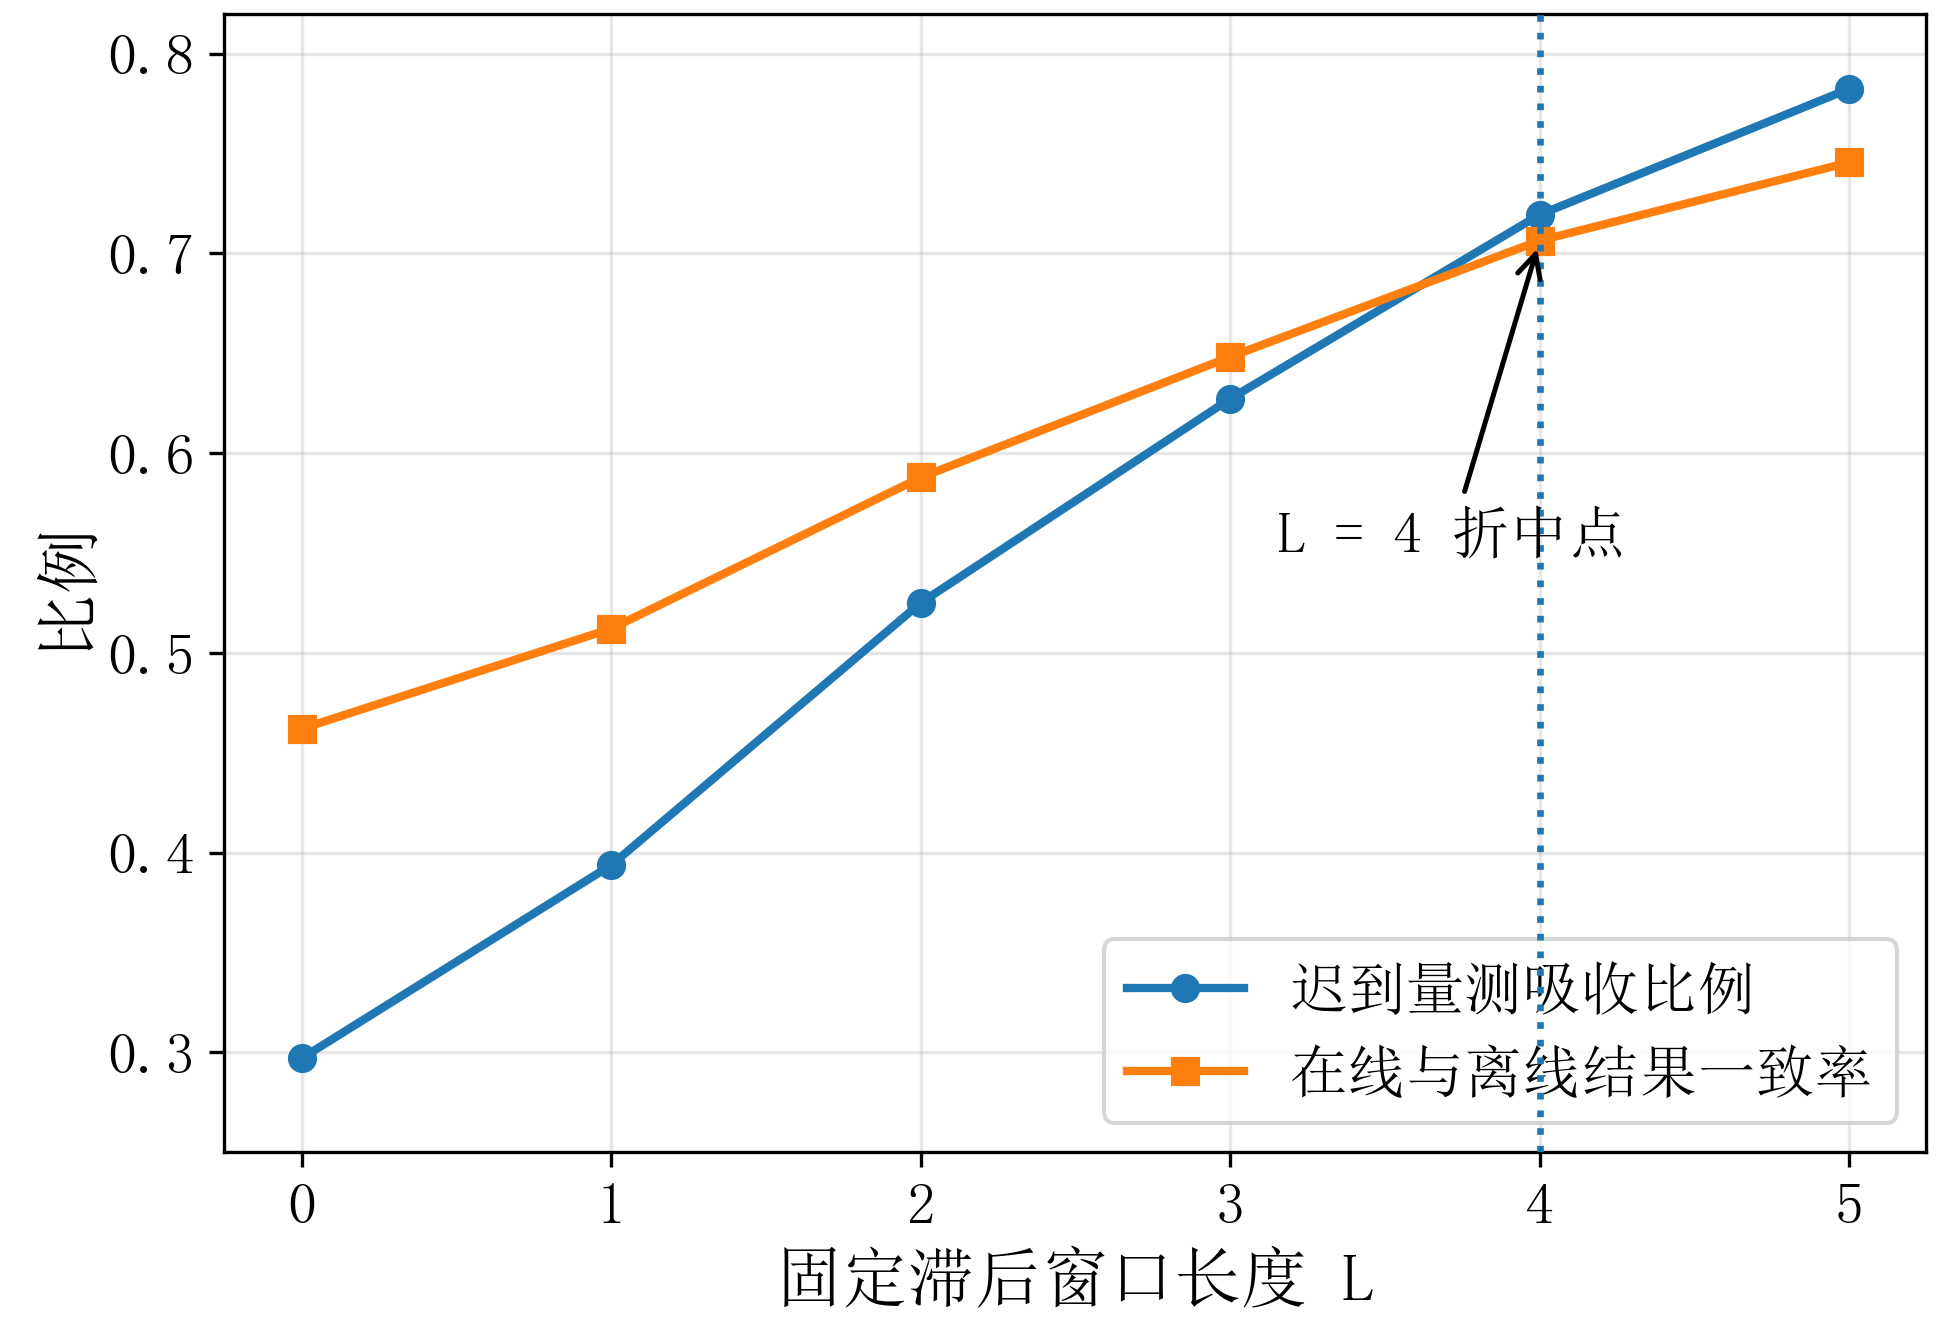
\includegraphics[width=0.80\textwidth]{code/chapter3/experiment1/exp1_results/3_12_merged_geomag_v2.png}
	\caption{固定滞后窗口长度对迟到量测吸收比例和与离线一致率结果图}
	\label{fig:ch3_exp5_time}
\end{figure}

图~\ref{fig:ch3_exp5_time} 给出了不同固定滞后窗口长度下两项指标的变化情况。随着 $L$ 由 $0$ 增加到 $5$，迟到量测吸收比例由 $0.297$ 提升至 $0.782$，结果一致率由 $0.462$ 提升至 $0.746$。当 $L=0$ 时，迟到量测吸收比例仍接近 $0.30$，说明部分跨扫描到达的地磁量测虽然晚于其所属扫描进入后台，但在扫描最终提交之前仍有机会被纳入处理。随着窗口增大，系统能够保留更长的历史扫描并执行更深的局部回放，更多会影响关联关系的迟到量测被重新吸收，因此两项指标都持续上升。需要注意的是，当 $L$ 从 $4$ 增加到 $5$ 时，收益已明显减弱，而缓存占用、局部回放计算量和在线输出时延仍会继续增加。综合收益与开销两方面因素，本文后续实验统一取 $L=4$ 作为默认配置。

\subsection{地磁传感器检测可靠性建模与自适应更新验证}

本节在 3.7.1 的双车道仿真路段和基础车辆生成方式上引入地磁传感器状态随时间变化的非平稳因素，用于验证检测概率与杂波空间密度后验的在线估计能力。仿真总时长设为 $T_{\mathrm{sim}}$，其中部分地磁传感器经历检测功能正常、退化和恢复三个阶段。相关参数见表~\ref{tab:ch3_node_adapt_sim}。检测功能退化区间内，对选中的 $N_{\mathrm{deg}}$ 个地磁传感器施加状态变化，其真实检测概率按 $P_{D,0}-0.48\zeta$ 下降，真实杂波空间密度按 $\lambda_{c,0}+0.12\zeta$ 增加；当时间超过 $t_2$ 后，再恢复到基准水平。除真实车辆地磁量测外，各扫描还按当前杂波强度生成无关地磁量测，从而同时模拟漏检增多和误触发增多两类退化现象。

\begin{table}[htbp]
	\centering
	\caption{地磁传感器检测可靠性建模实验的仿真参数设置}
	\label{tab:ch3_node_adapt_sim}
	\small
	\begin{tabular}{p{2.8cm}p{3.0cm}p{6.0cm}}
		\toprule
		参数 & 取值 & 参数含义 \\
		\midrule
		$T_{\mathrm{sim}}$ & $600\,\mathrm{s}$ & 仿真总时长 \\
		$N_{\mathrm{deg}}$ & 30 & 施加状态变化的地磁传感器数量 \\
		$t_1$ & $180\,\mathrm{s}$ & 退化开始时刻 \\
		$t_2$ & $390\,\mathrm{s}$ & 恢复开始时刻 \\
		$P_{D,0}$ & 0.94 & 基准检测概率 \\
		$\lambda_{c,0}$ & 0.015 & 基准杂波空间密度 \\
		$\zeta_{\mathrm{main}}$ & 0.70 & 代表性后验曲线的检测能力退化强度 \\
		$\zeta_{\mathrm{sweep}}$ & 0，0.25，0.5，0.75，1.0 & 性能统计的退化强度 \\
		$\Delta T$ & $0.8\,\mathrm{s}$ & 扫描时间片长度 \\
		$L$ & 4 & 固定滞后窗口长度 \\
		\bottomrule
	\end{tabular}
\end{table}

本节比较三种方法。第一种为规则基线方法，在全部地磁传感器上的检测概率与杂波强度使用固定可靠性参数，不进行后验估计；第二种为全局统一后验方法，保留本文的关联与轨迹管理流程，但不再对不同地磁传感器分别维护检测概率和杂波空间密度后验，而是让全部地磁传感器共享同一组统一后验参数。第三种为本文方法，即对每个地磁传感器分别维护检测概率和杂波空间密度后验，并在扫描内数据处理结果全部提交后利用软计数进行在线更新。实验中从退化地磁传感器中选取一个代表性地磁传感器绘制后验曲线，同时在不同退化强度下统计身份切换次数和误删轨迹次数。

\begin{figure}[htbp]
	\centering
	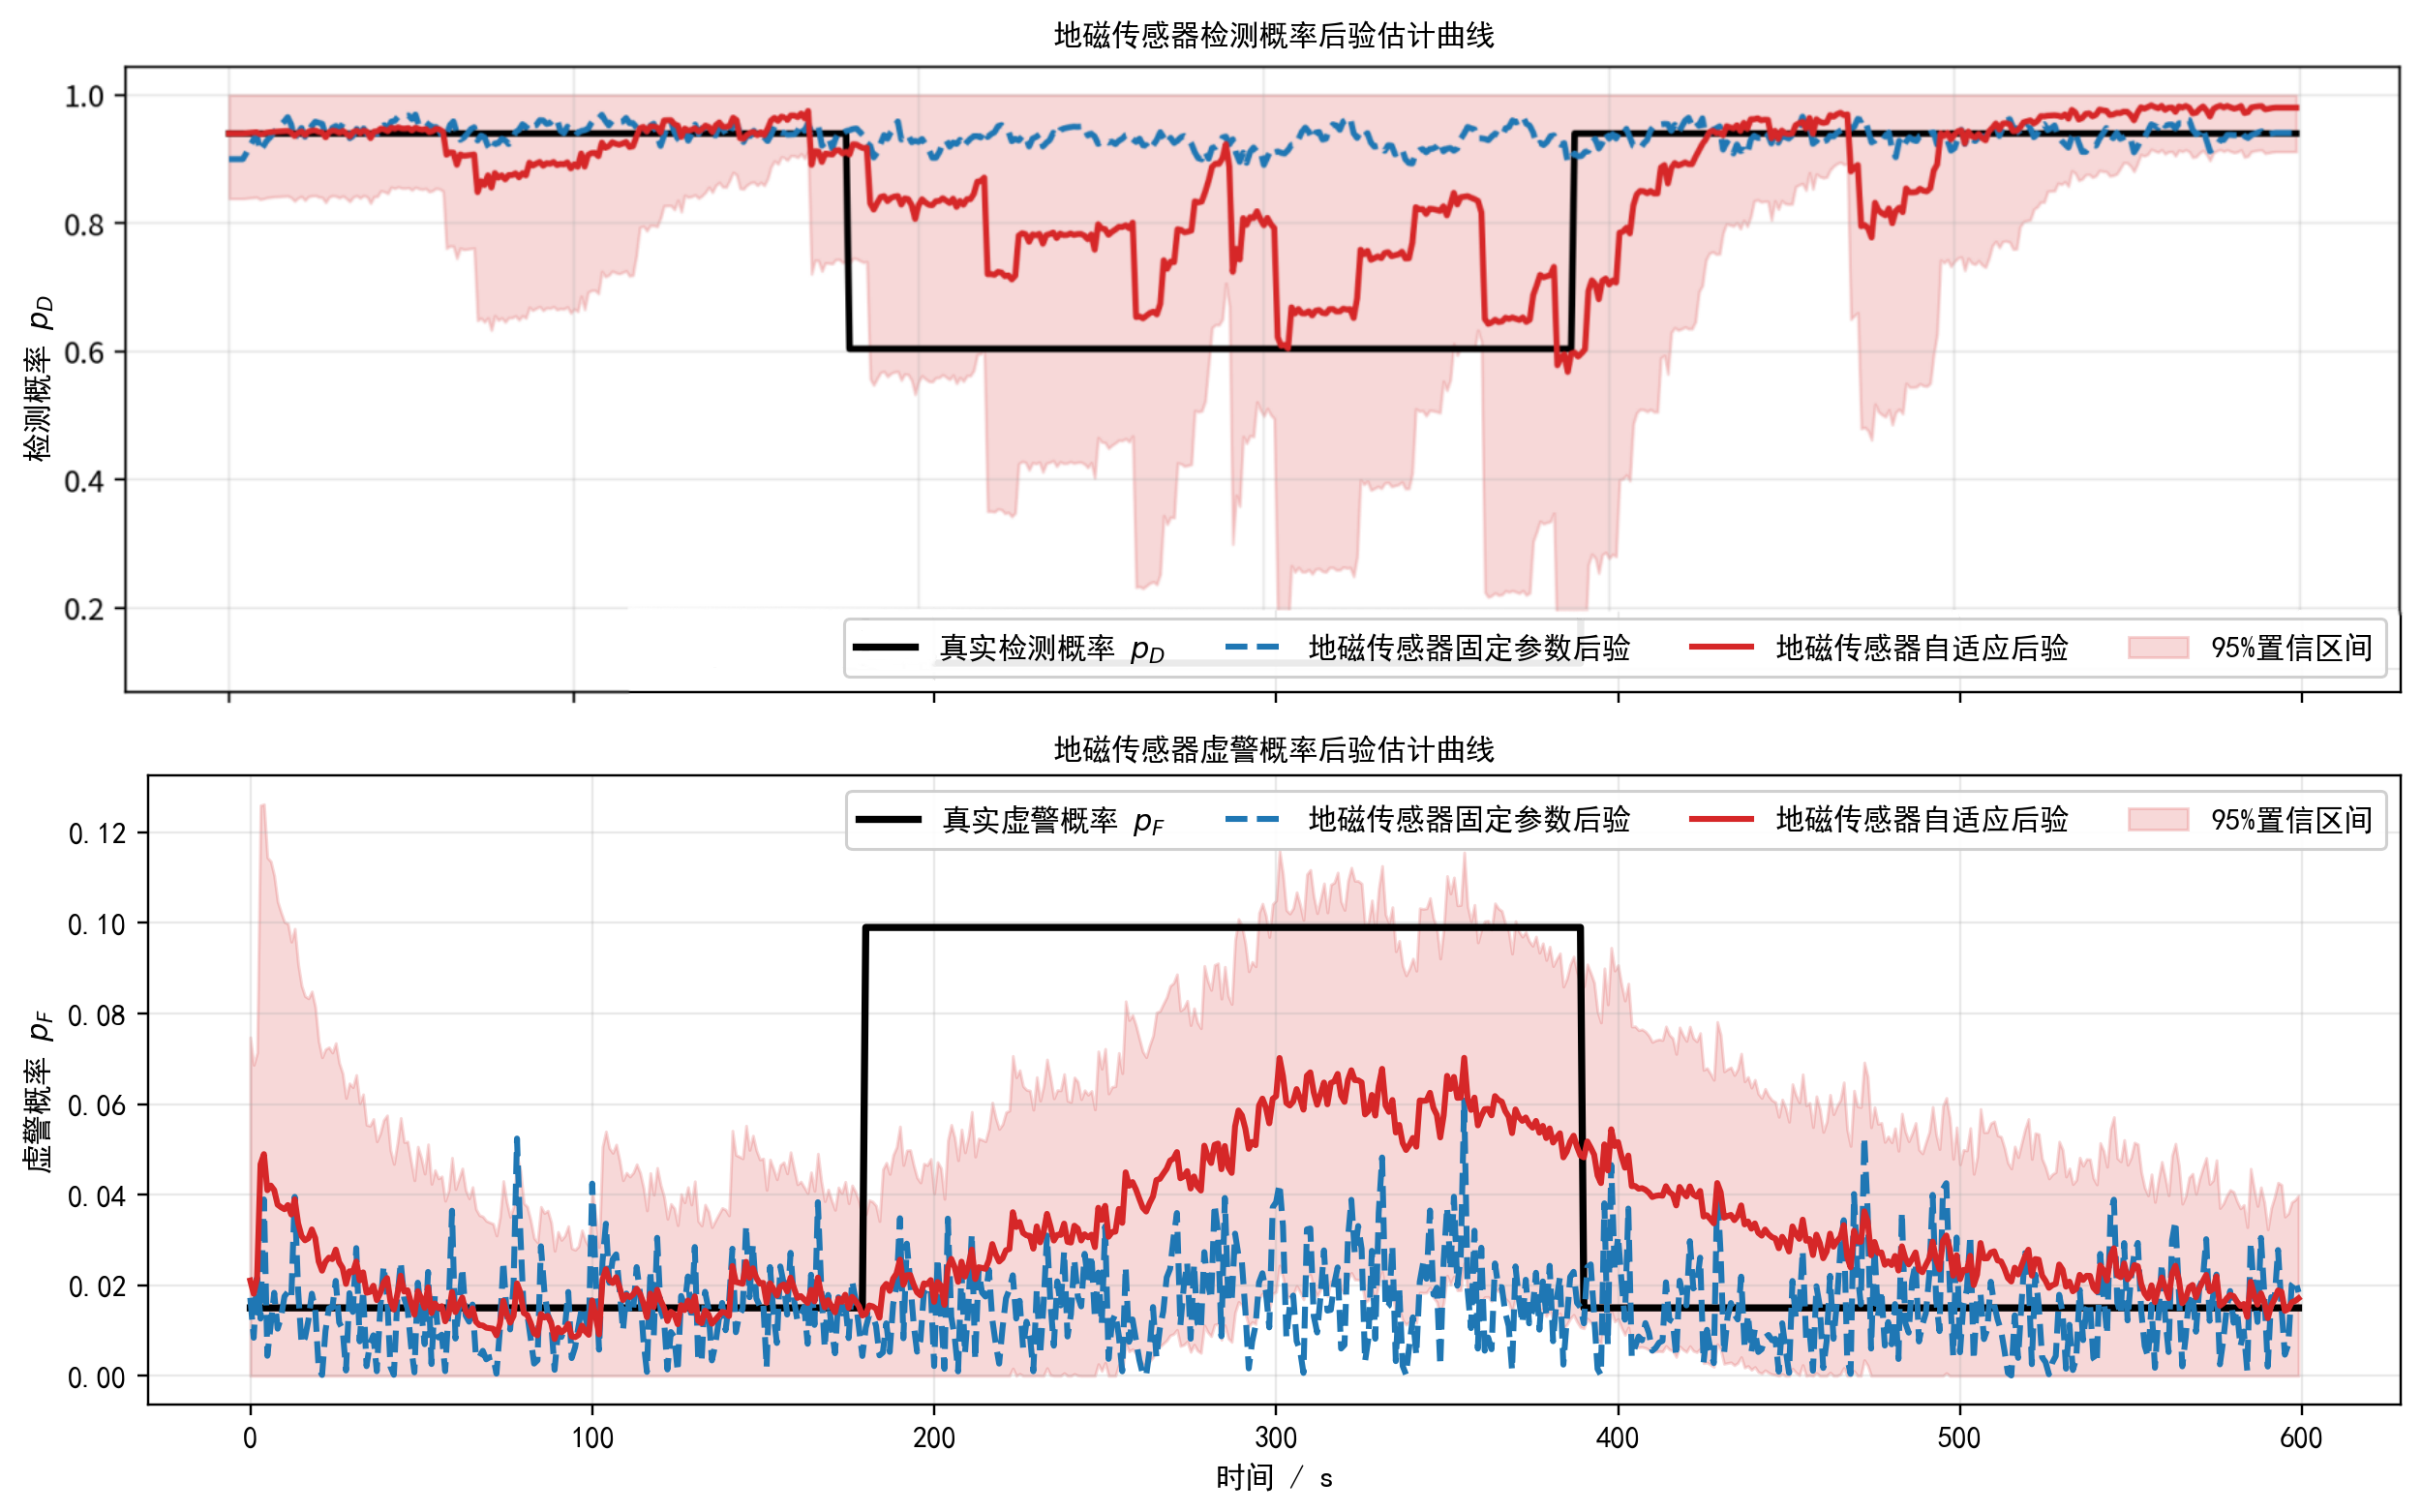
\includegraphics[width=0.88\textwidth]{code/chapter3/experiment1/exp1_results/3_7_exp1_node_posterior_curve.png}
	\caption{地磁传感器检测概率与杂波强度的后验估计结果图}
	\label{fig:ch3_exp2_node_posterior}
\end{figure}

\begin{figure}[htbp]
	\centering
	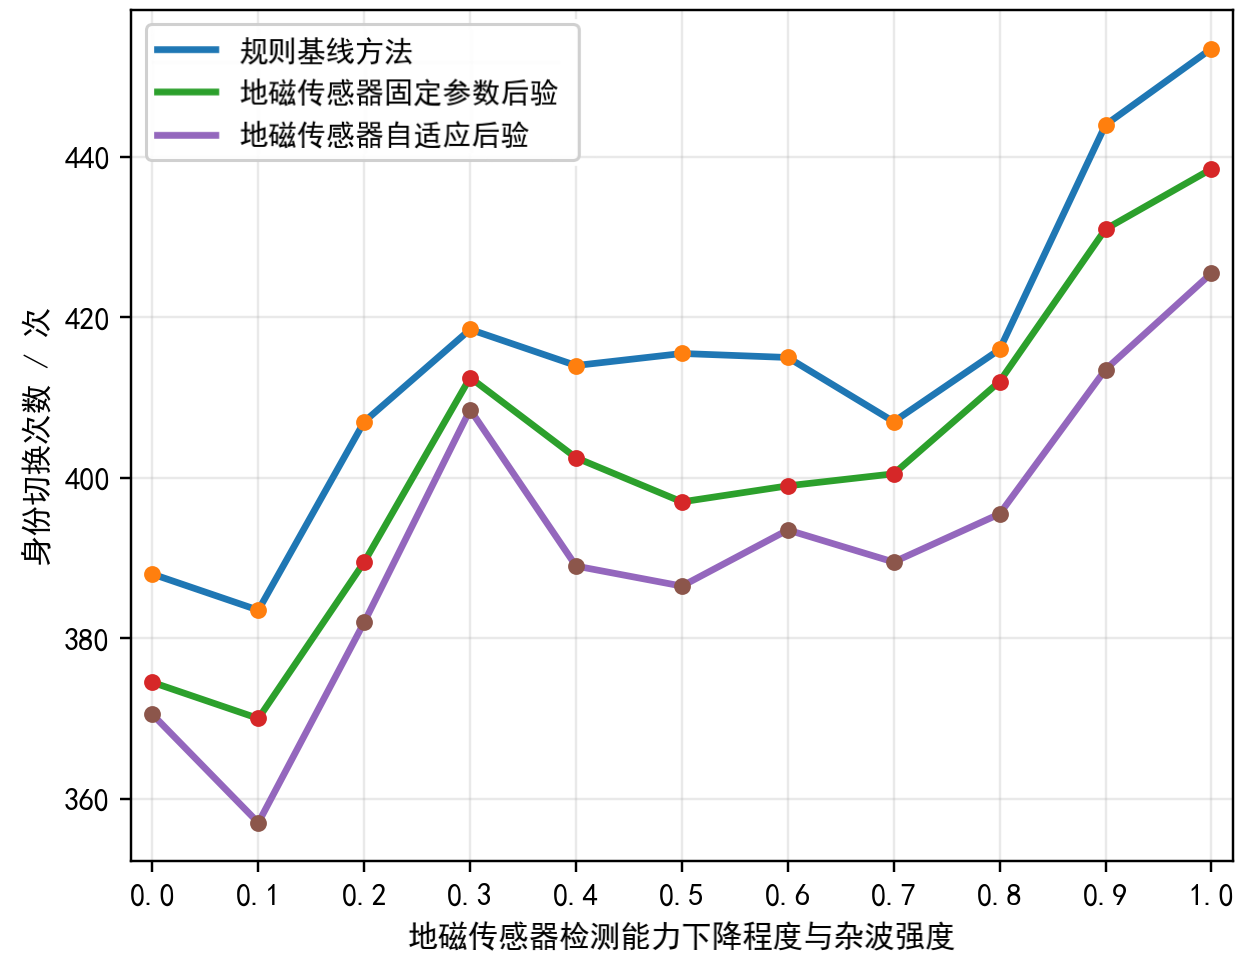
\includegraphics[width=0.60\textwidth]{code/chapter3/experiment1/exp1_results/3_8_1_exp1_degradation_impact_v1.png}
	\caption{不同地磁传感器检测能力下降程度与杂波强度下身份切换次数图}
	\label{fig:ch3_exp1_idsw}
\end{figure}

\begin{figure}[htbp]
	\centering
	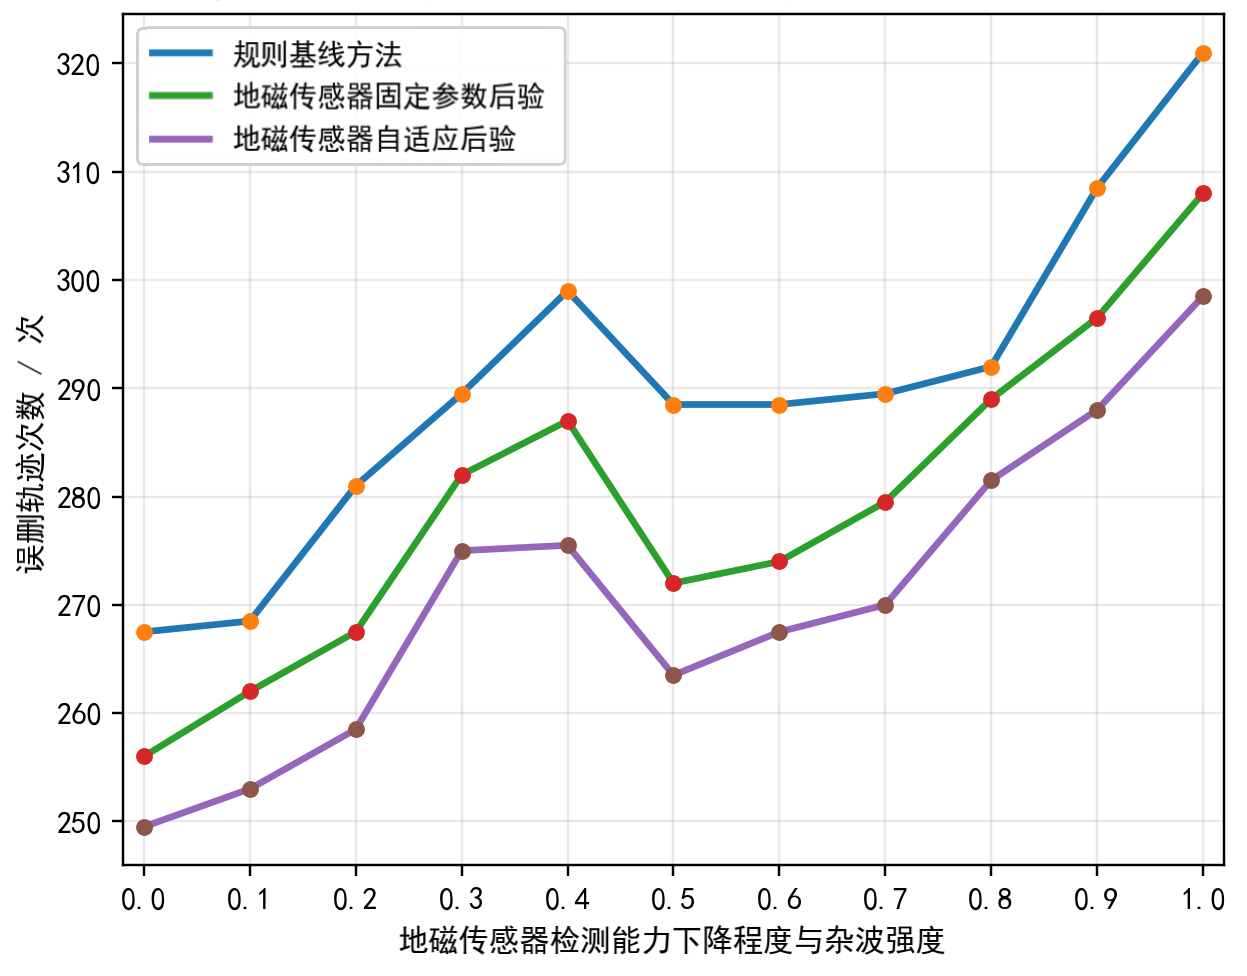
\includegraphics[width=0.60\textwidth]{code/chapter3/experiment1/exp1_results/3_8_2_exp1_degradation_impact_v1.png}
	\caption{不同地磁传感器检测能力下降程度与杂波强度下误删轨迹次数图}
	\label{fig:ch3_exp1_false_delete}
\end{figure}

图~\ref{fig:ch3_exp2_node_posterior} 给出了一组代表性退化地磁传感器的检测概率与杂波强度后验估计结果。可从图中看出，本文方法能够较快跟随检测性能退化地磁传感器检测概率的下降与恢复过程，对杂波强度的抬升和回落也有较清晰响应；相比之下，全局统一后验对局部退化的响应明显滞后。图~\ref{fig:ch3_exp1_idsw} 和图~\ref{fig:ch3_exp1_false_delete} 进一步表明，随着地磁传感器检测能力下降和杂波增强，各方法的身份切换次数与误删轨迹次数都会增加，但本文方法在不同退化强度下始终保持最低水平，且增长幅度更缓。这说明地磁传感器状态自适应后验不仅能提高参数辨识能力，也能为后续关联和轨迹管理提供更可靠的先验支持。

\subsection{邻道干扰与双车并行场景判别验证}

本节不再生成完整的在线跟踪数据流，而是单独构造面向场景判别的双侧地磁量测序列，以便直接考察场景后验递推对邻道干扰和双车并行的区分能力。每条序列沿车辆行驶方向连续经过 $N_{\mathrm{pair}}$ 对地磁传感器，相邻地磁传感器间距为 $L_a$。相关参数见表~\ref{tab:ch3_scene_discrim_sim}。实验共构造三类典型序列：单车正常通过序列、单车通过并伴随邻道干扰序列，以及困难双车并行序列。最后一种情况最容易与邻道干扰混淆，因此用来重点考察方法的稳定判别能力。

\begin{table}[htbp]
	\centering
	\caption{场景判别实验的仿真参数设置}
	\label{tab:ch3_scene_discrim_sim}
	\small
	\begin{tabular}{p{2.8cm}p{3.0cm}p{6.0cm}}
		\toprule
		参数 & 取值 & 参数含义 \\
		\midrule
		$N_{\mathrm{pair}}$ & 18 & 连续地磁传感器对数量 \\
		$N_{\mathrm{seq}}$ & 60 & 每类场景的样本序列数 \\
		$L_a$ & $15\,\mathrm{m}$ & 相邻地磁传感器间距 \\
		$\bar v$ & $22\,\mathrm{m/s}$ & 基础车速 \\
		$\sigma_t$ & $25\,\mathrm{ms}$ & 双侧触发时间噪声标准差 \\
		$p_{\mathrm{adj}}$ & 0.88 & 邻道干扰触发概率 \\
		$\Delta t_{\mathrm{adj}}$ & $\mathcal N(120,70^2)\,\mathrm{ms}$ & 邻道干扰时间偏移 \\
		$\kappa_{\mathrm{adj}}$ & 0.40 & 邻道干扰峰值比例 \\
		$|\Delta v_{\mathrm{par}}|$ & $\leq 1.5\,\mathrm{m/s}$ & 双车并行速度差上界 \\
		$p_{\mathrm{drop}}$ & 0.04 & 并行样本单侧偶发缺失概率 \\
		\bottomrule
	\end{tabular}
\end{table}

本节比较三类方法。第一类为单帧阈值规则方法，仅依据当前地磁传感器对的触发时间差和地磁峰值差异直接作出场景判别。第二类为单帧概率判别方法，仅利用当前地磁传感器对上的概率输出进行决策，不进行跨扫描递推。第三类为本文方法，即在固定滞后窗口内对场景后验进行多步递推，通过连续多个地磁传感器上的弱判别证据逐步形成稳定场景结论。在全部仿真样本中，另外从困难双车并行序列中选取一个最具代表性的样本，绘制图~\ref{fig:ch3_exp3_hard_case} 所示的场景后验递推过程，用于直观展示不同方法在临界并行情形下的判别差异。

\begin{figure}[htbp]
	\centering
	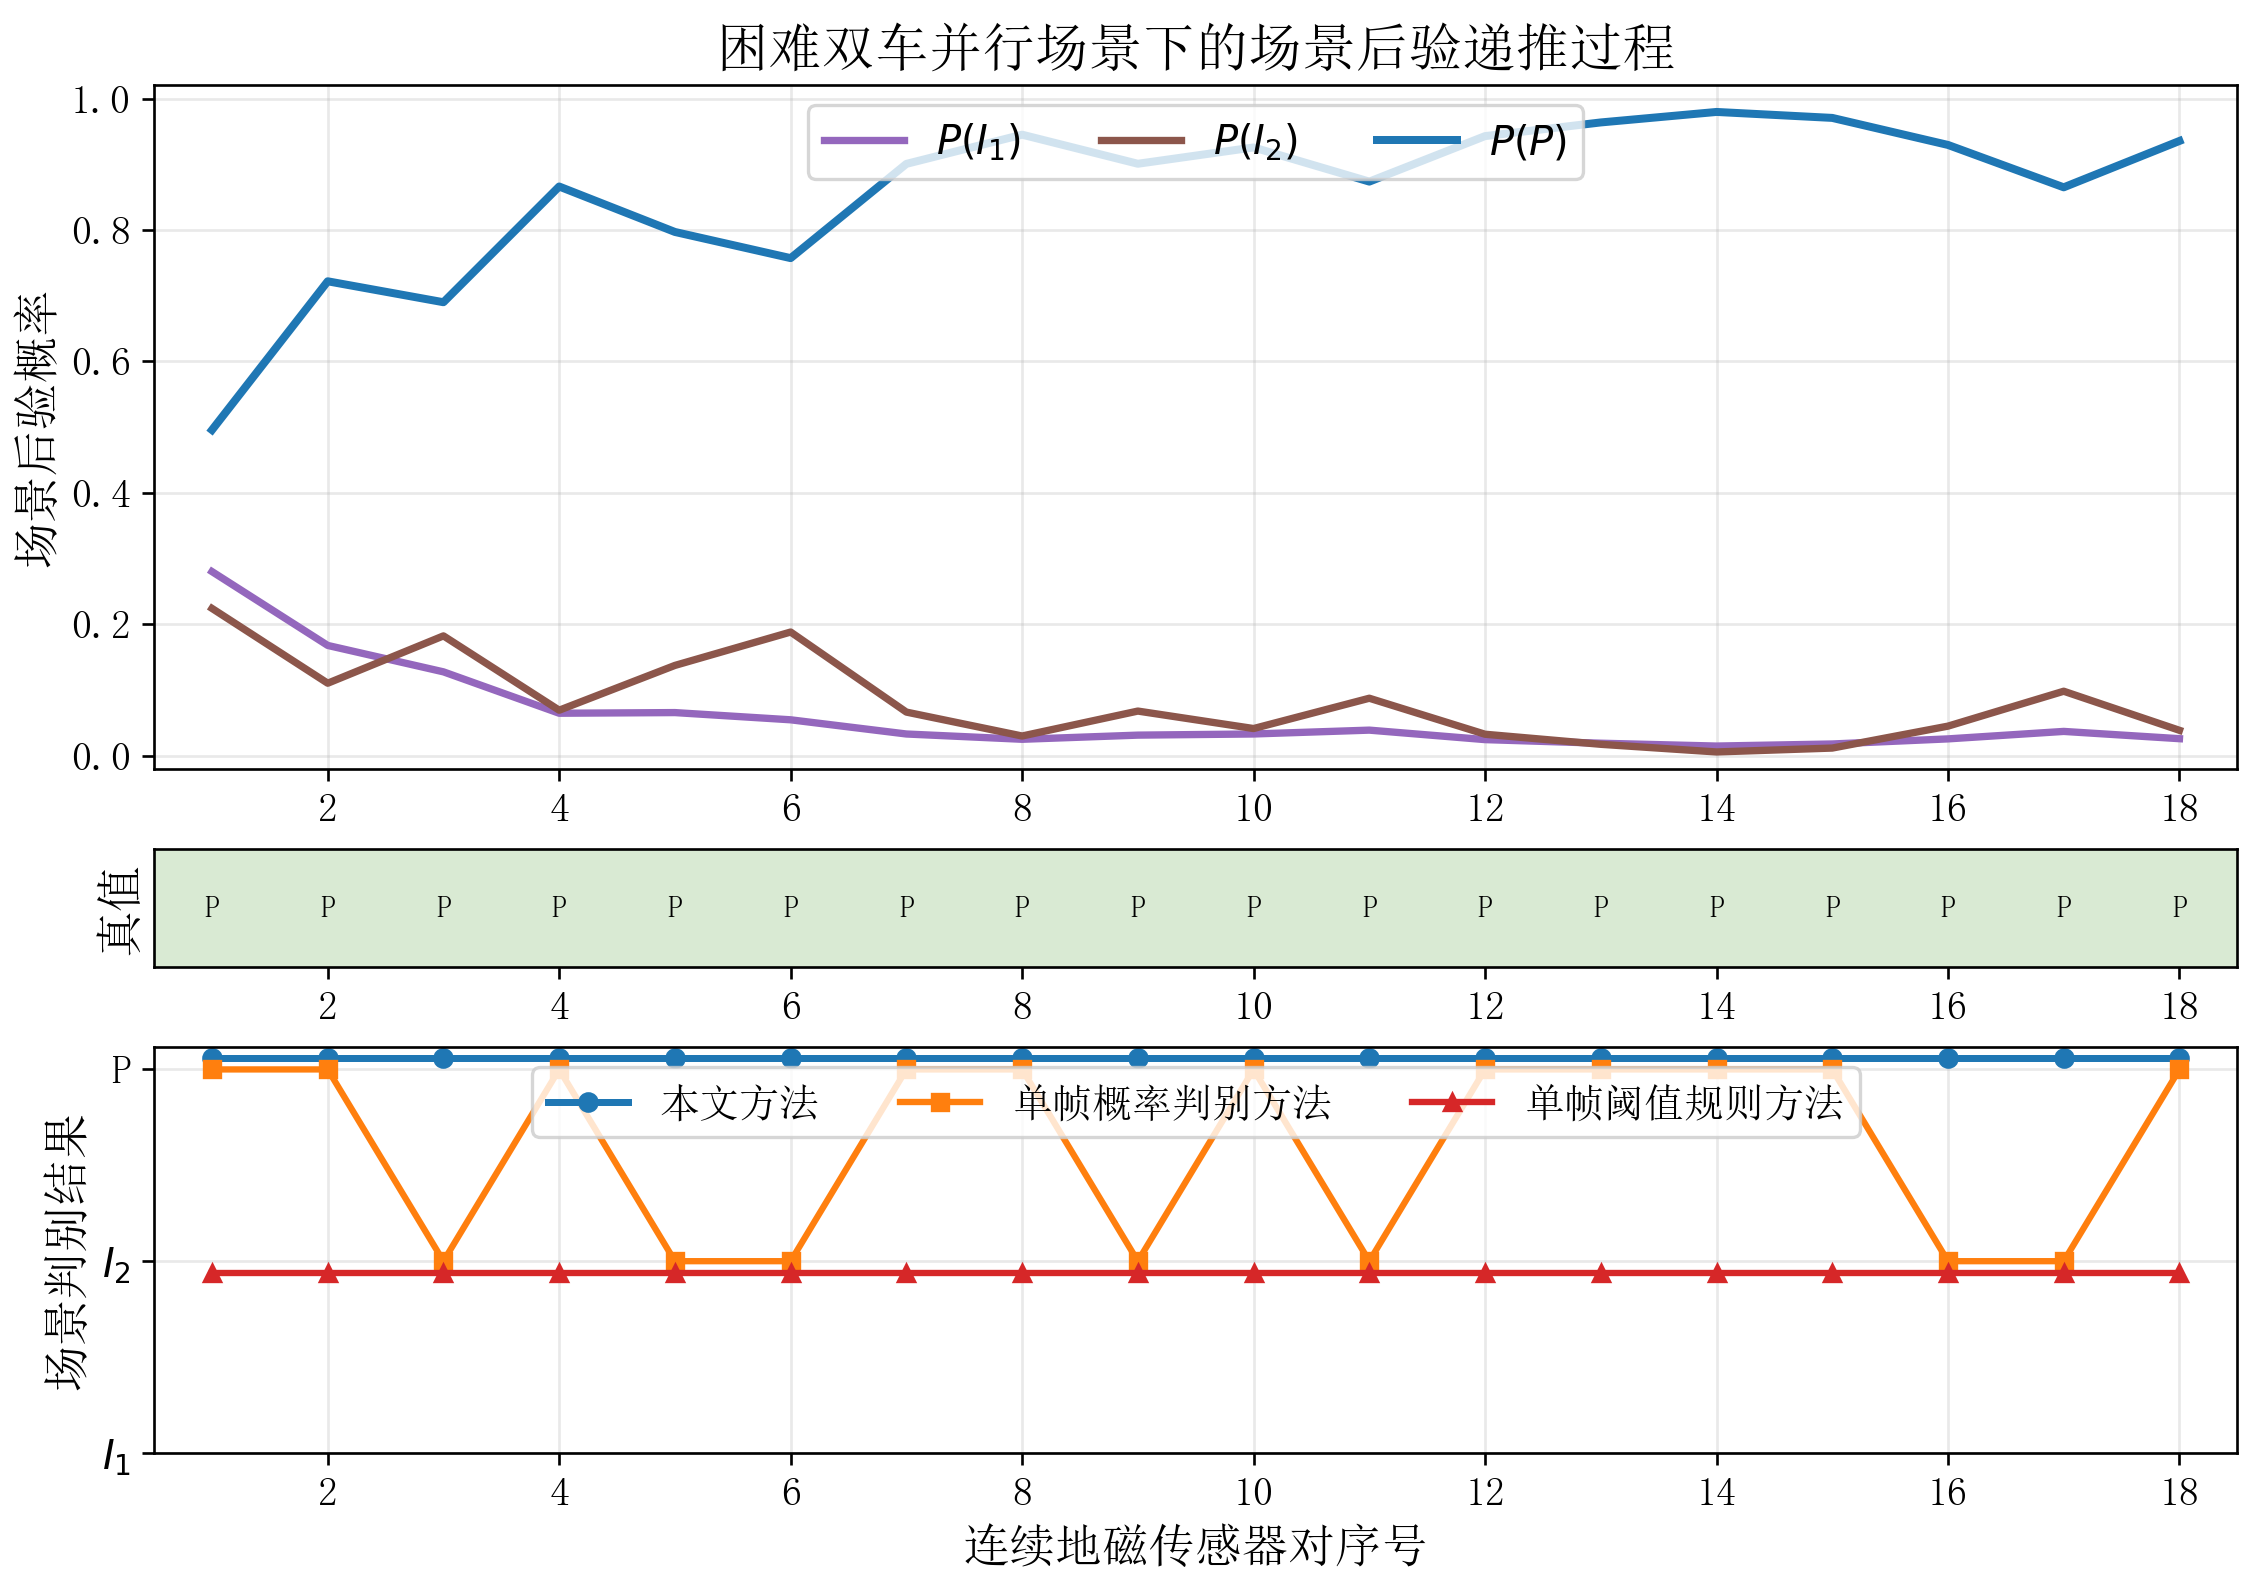
\includegraphics[width=0.88\textwidth]{code/chapter3/experiment1/exp1_results/3_9_hard_parallel_tuned_v2.png}
	\caption{困难双车并行场景下的场景后验递推结果图}
	\label{fig:ch3_exp3_hard_case}
\end{figure}

图~\ref{fig:ch3_exp3_hard_case} 给出了一个困难双车并行样本的场景后验递推过程。该样本的初始横向间隔约为 $1.4\,\mathrm{m}$，速度差范围为 $0.07$ 至 $1.30\,\mathrm{m/s}$，双侧相对时间差范围为 $1$ 至 $56\,\mathrm{ms}$，未注入换道动作，连续经过 $18$ 对地磁传感器。可以看到，在该类临界并行情形下，单帧阈值规则方法在整个地磁传感器序列上几乎始终停留在邻道干扰状态，未能恢复真实双车并行关系；单帧概率判别方法虽然在部分地磁传感器对处能够给出正确判断，但其结果在相邻地磁传感器对之间仍存在明显波动，难以形成稳定场景结论。相比之下，本文方法在前期若干地磁传感器对上完成多步证据累积后，双车并行状态后验逐步占优，并在后续区间内保持较高稳定性。该结果表明，当双侧相对时间差持续较小、地磁扰动峰值差异又不足以单独支撑硬判决时，仅依赖单次观测进行判别，容易将真实双车并行误判为邻道干扰，或者在两种场景之间反复切换；而引入状态持续性约束与多步场景后验递推后，算法能够利用连续多个地磁传感器对上的弱判别信息逐步拉开不同场景的后验差异，从而显著缓解上述失效模式。

\subsection{车道状态更新与修正验证}

本节复用表~\ref{tab:ch3_scene_discrim_sim} 中的基础序列生成方式，并在此基础上增加带换道动作的扩展样本，以验证场景后验进入车道状态递推后的稳定性。除三类基础序列外，额外生成 $N_{\mathrm{lc}}=30$ 组换道扩展序列。对每条换道序列，车辆在中段连续 $3$ 至 $4$ 对地磁传感器范围内完成由旧车道到新车道的过渡，换道起始位置在第 $7$ 至第 $11$ 对地磁传感器之间随机抽样。最终评测集由基础序列和换道扩展序列共同组成。

本节对比的方法见表~\ref{tab:ch3_method_def}。前三类方法直接面向场景判别与车道状态更新设计，后三类方法则先给出轨迹级关联结果，再映射为可比较的场景与车道标签。对每条样本序列，分别统计场景判别准确率、车道状态准确率、真实双车并行被误判为邻道干扰的比例，以及车道状态抖动次数。

\begin{table}[htbp]
	\centering
	\caption{场景判别与车道状态更新对比方法}
	\label{tab:ch3_method_def}
	\small
	\begin{tabular}{p{4.0cm}p{7.2cm}}
		\toprule
		方法名称 & 主要特点 \\
		\midrule
		本文方法 & 多步场景后验递推，地磁传感器可靠性自适应建模，场景后验进入车道状态更新 \\
		单帧概率判别方法 & 仅利用当前地磁量测的概率输出，不进行跨扫描递推 \\
		单帧阈值规则方法 & 仅利用当前地磁量测的阈值硬判决 \\
		地磁传感器固定参数后验方法 & 保留递推结构，但地磁传感器可靠性采用全局固定参数 \\
		JPDA 结合 KF 方法 & 轨迹级软关联，场景标签由双侧轨迹结果后处理映射得到 \\
		MHT 结合 KF 方法 & 轨迹级多假设关联，场景标签由双侧轨迹结果后处理映射得到 \\
		\bottomrule
	\end{tabular}
\end{table}

图~\ref{fig:ch3_exp3_metrics} 汇总了上述方法在场景判别与车道状态更新任务上的整体结果，包括场景判别准确率、车道状态准确率、真实双车并行被误判为邻道干扰的比例，以及车道状态抖动次数。

\begin{figure}[htbp]
	\centering
	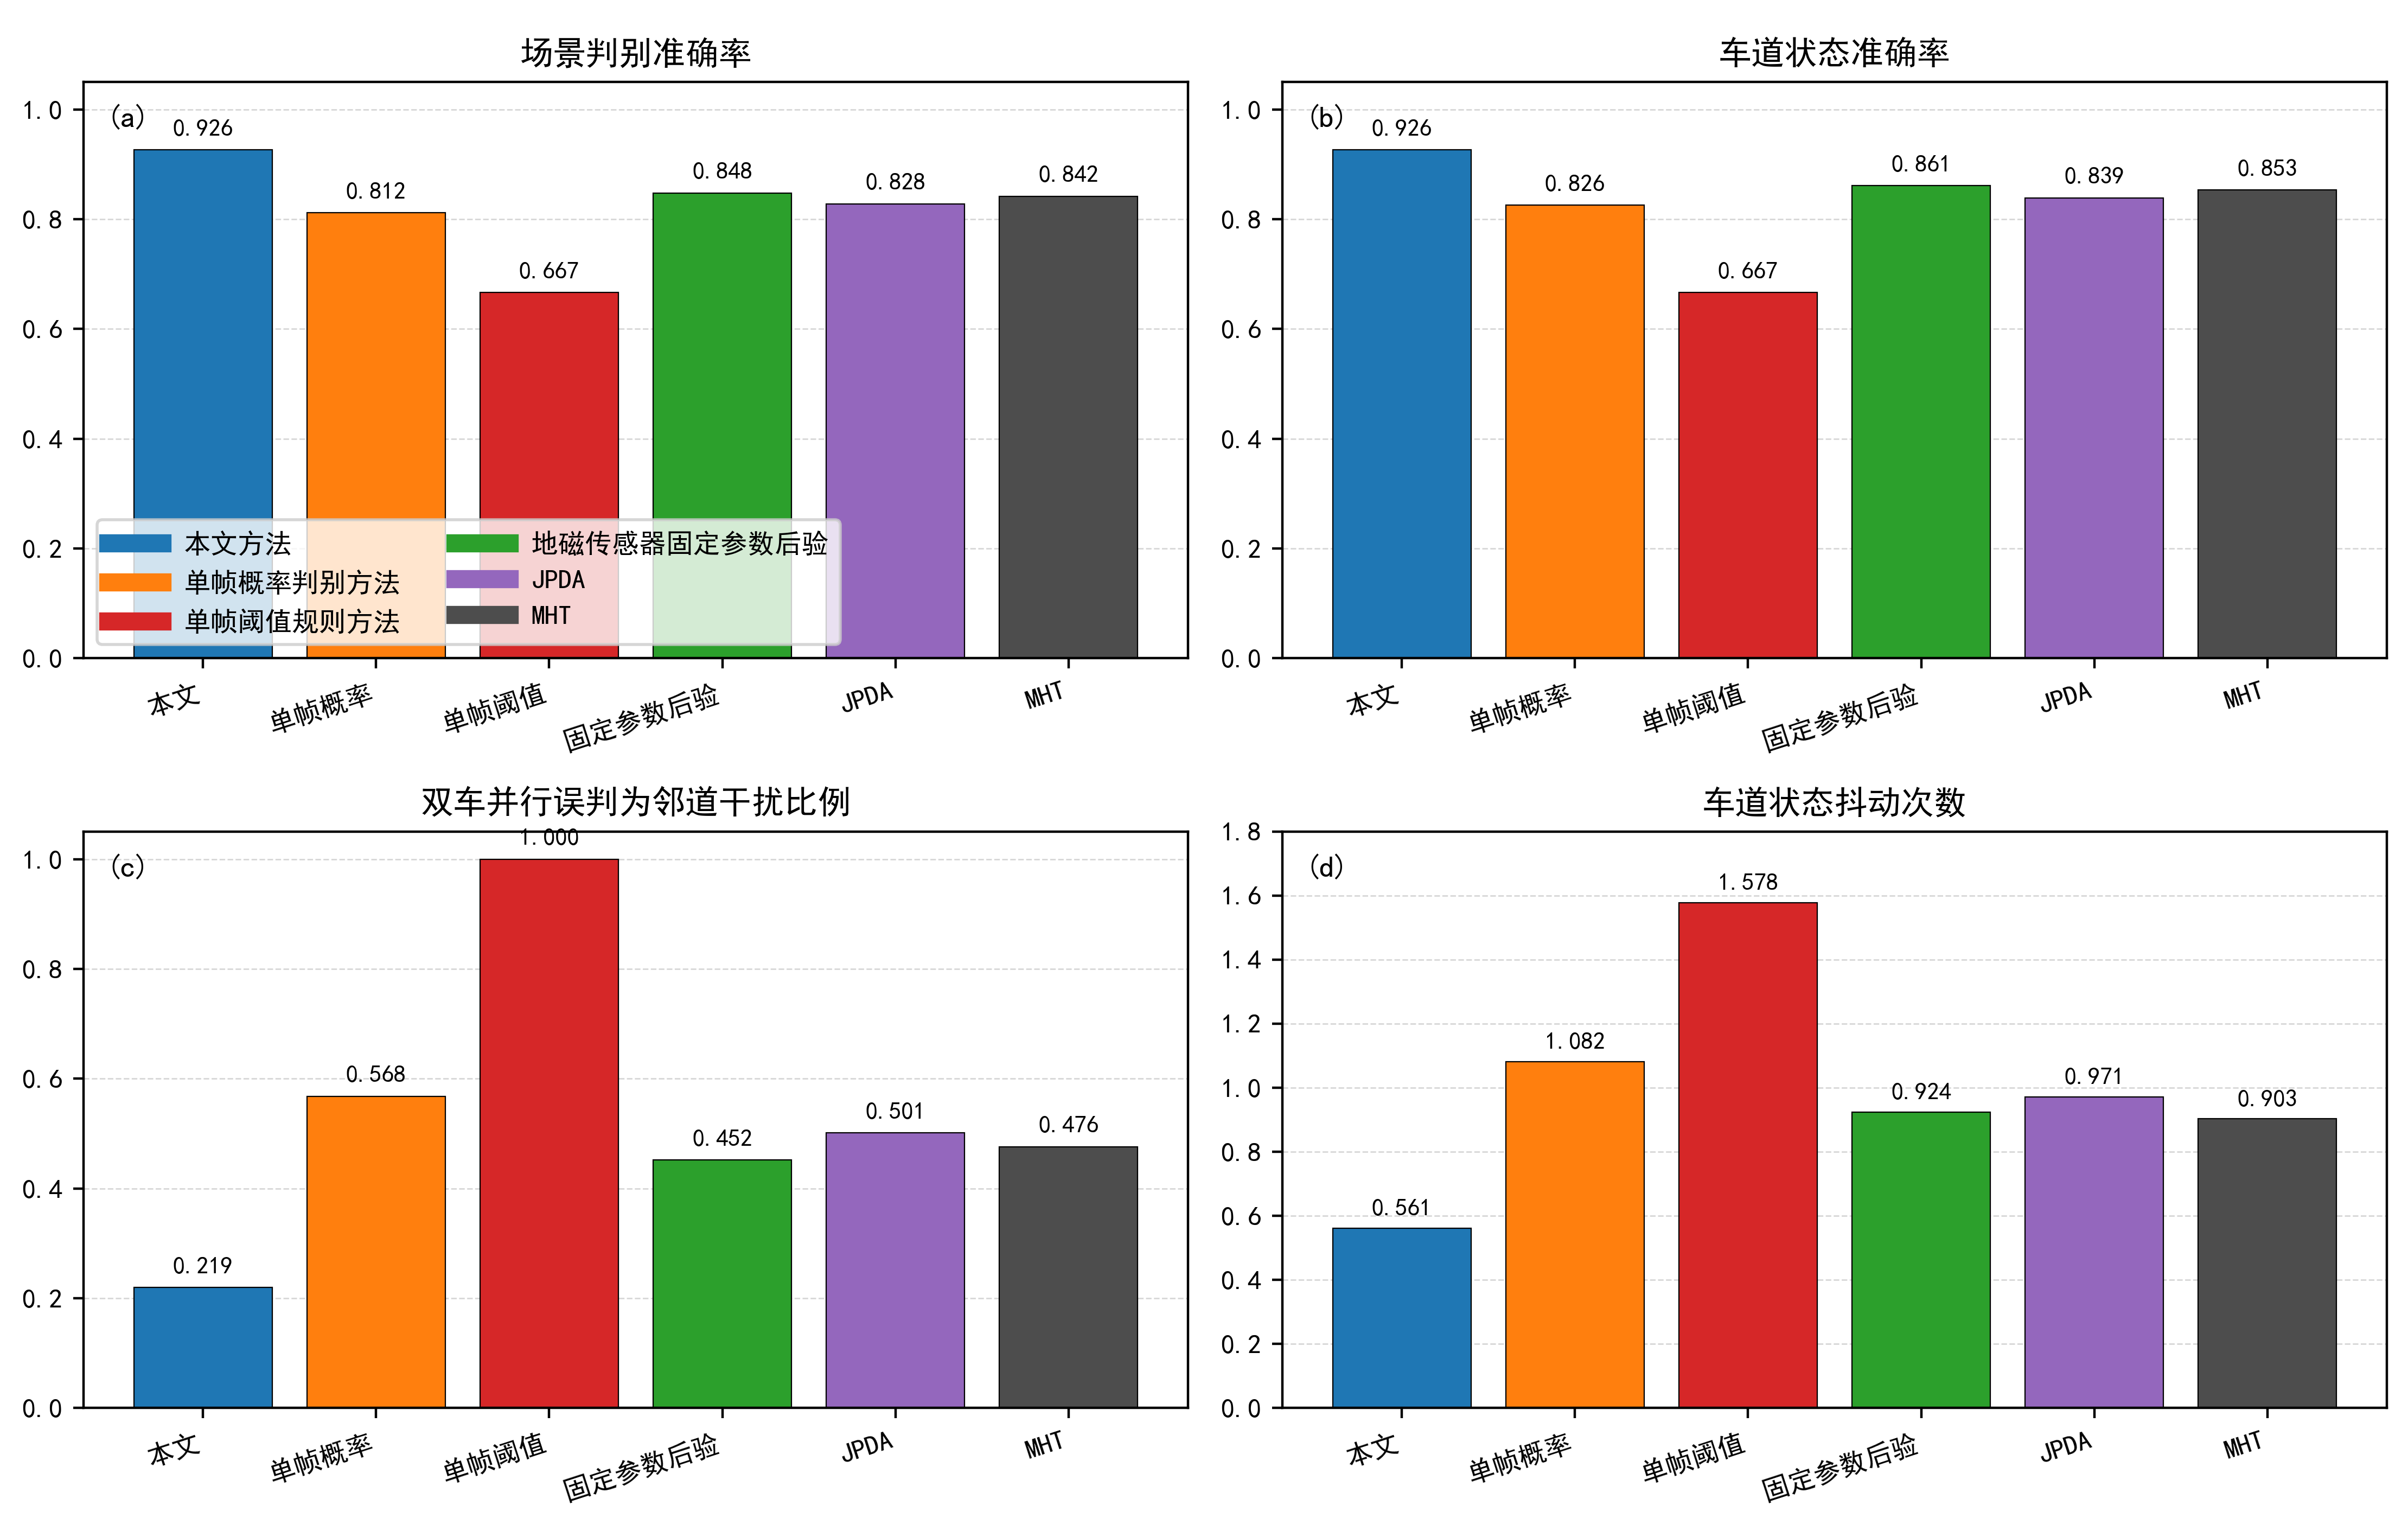
\includegraphics[width=0.92\textwidth]{code/chapter3/experiment1/exp1_results/3_10_multi_algo_scene_metrics.png}
	\caption{多算法场景判别与车道状态指标对比图}
	\label{fig:ch3_exp3_metrics}
\end{figure}

从图中可以看到，地磁传感器固定参数后验、JPDA 结合 KF 和 MHT 结合 KF 的表现整体介于本文方法与两类单帧方法之间。这说明仅在轨迹级关联层面改进，或者仅在全局层面使用统一可靠性参数，虽然能够在一定程度上改善结果，但仍难以替代场景后验直接进入车道状态更新所带来的优势。其次，从最容易失效的双车并行场景看，单帧阈值规则方法将真实双车并行误判为邻道干扰的比例达到 $1.0000$，说明其在两车近同步通过时几乎失去区分能力；本文方法将该比例显著降低至 $0.2194$。表明三状态场景后验递推能够有效修正单帧规则在复杂并行场景中的系统性偏差，使邻道干扰和真实双车并行的判别不再仅依赖某一次局部观测，而是建立在多时刻证据累积的基础上。最后，从输出稳定性看，本文方法的车道状态抖动次数由 $1.5778$ 降至 $0.5611$，表明本文方法的优势不仅体现在判别更准确，还体现在车道状态更新更加平滑、连续。尤其是在注入换道动作的扩展样本中，当场景后验进入车道状态递推后，车道后验能够在固定滞后窗口内完成由旧车道到新车道的平滑翻转，而不会因单次对侧弱触发而产生误切换或反复回摆。这一点与图~\ref{fig:ch3_exp3_metrics} 中车道状态抖动次数显著下降的结果是一致的。



\subsection{目标跟踪综合性能对比}

本节采用完整双车道异步地磁量测流作为输入。时间组织参数沿用 3.7.1，地磁传感器退化与杂波建模沿用 3.7.2，邻道干扰与双车并行构造沿用 3.7.3，并在此基础上形成三类难度递增的评测场景。三种场景的差异主要体现在地磁传感器检测性能退化强度、杂波水平、双车并行比例、邻道弱触发概率以及车流密度五个方面，具体设置见表~\ref{tab:ch3_tracking_scene_setup}。

\begin{table}[htbp]
	\centering
	\caption{目标跟踪综合性能对比实验的场景设置}
	\label{tab:ch3_tracking_scene_setup}
	\small
	\begin{tabular}{p{1.8cm}p{2.2cm}p{2.0cm}p{2.0cm}p{2.2cm}p{2.3cm}}
		\toprule
		场景 & 退化强度 $\zeta$ & 杂波水平 & 双车并行比例 & 邻道弱触发概率 & 同车道进入时间间隔 \\
		\midrule
		场景 A & 0.35 & $1.0\lambda_{c,0}$ & 0.15 & 0.20 & $[2.5,4.0]\,\mathrm{s}$ \\
		场景 B & 0.55 & $1.6\lambda_{c,0}$ & 0.25 & 0.35 & $[1.8,3.2]\,\mathrm{s}$ \\
		场景 C & 0.75 & $2.2\lambda_{c,0}$ & 0.35 & 0.50 & $[1.2,2.5]\,\mathrm{s}$ \\
		\bottomrule
	\end{tabular}
\end{table}

本节在统一的常速度 Kalman 滤波状态表示下，对比本文方法、JPDA 结合 KF 方法和和航迹导向多假设跟踪（Track-Oriented Multiple Hypothesis Tracking，TOMHT）结合 KF 方法。三种方法采用相同的地磁传感器触发位置伪观测形式和一致的常速度状态模型，差异主要体现在关联层。每个场景独立重复仿真 $15$ 次，对各方法输出的有效轨迹点按照真实车辆身份与真实状态进行对齐，统计位置均方根误差 $RMSE_p$ 和速度均方根误差 $RMSE_v$，并对重复结果取平均值。

\begin{figure}[htbp]
	\centering
	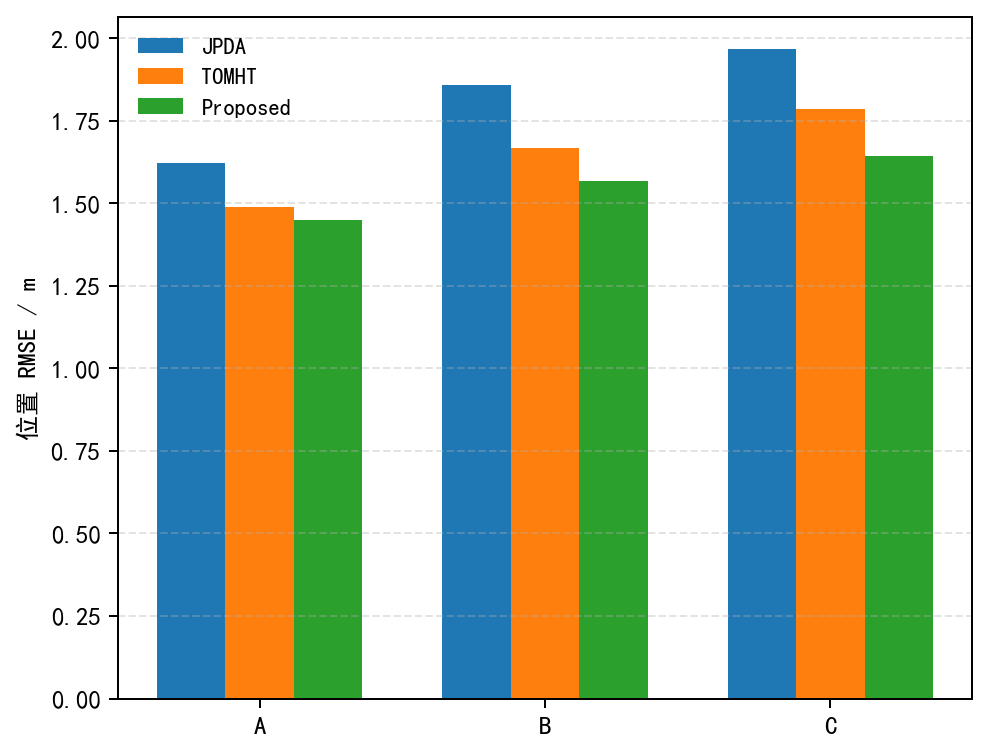
\includegraphics[width=0.58\textwidth]{code/chapter3/experiment1/exp1_results/ch3_tracking_accuracy_rmse_p.png}
	\caption{三类复杂场景下不同算法的位置 RMSE 对比图}
	\label{fig:ch3_tracking_accuracy_rmse_p}
\end{figure}

\begin{figure}[htbp]
	\centering
	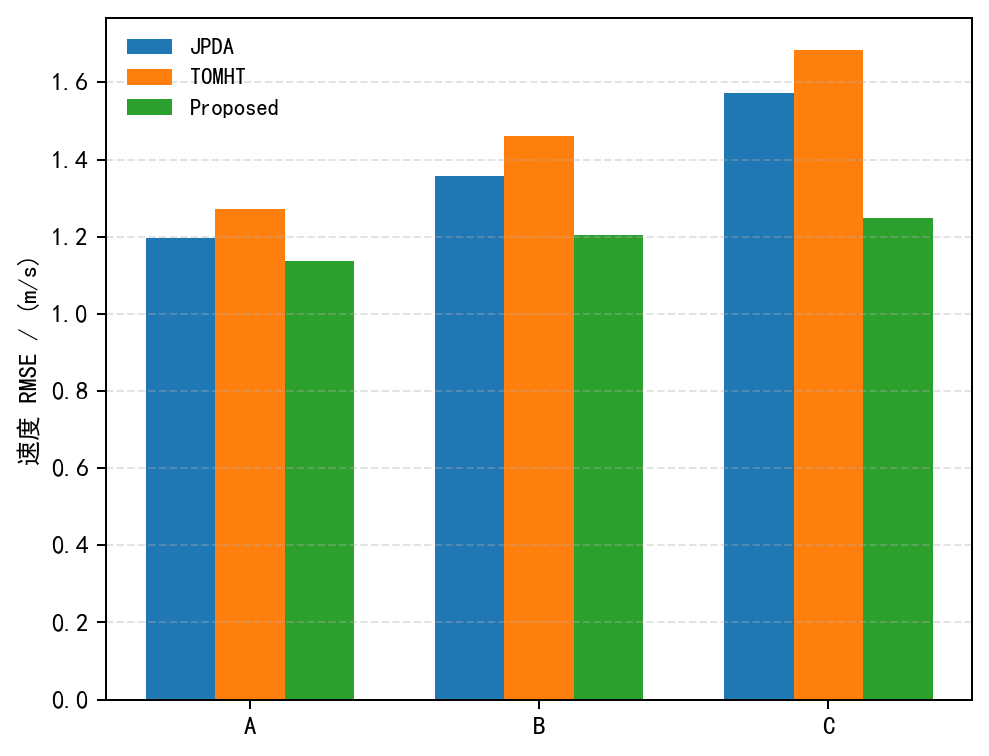
\includegraphics[width=0.58\textwidth]{code/chapter3/experiment1/exp1_results/ch3_tracking_accuracy_rmse_v.png}
	\caption{三类复杂场景下不同算法的速度 RMSE 对比图}
	\label{fig:ch3_tracking_accuracy_rmse_v}
\end{figure}

图~\ref{fig:ch3_tracking_accuracy_rmse_p} 和图~\ref{fig:ch3_tracking_accuracy_rmse_v} 表明，随着场景复杂度由场景 A 提升到场景 C，三种方法的位置与速度误差都会增大，但本文方法在三类场景下始终保持最优。以最困难的场景 C 为例，本文方法的位置 $RMSE$ 为 $1.6426\,\mathrm{m}$，优于 JPDA 结合 KF 方法的 $1.9668\,\mathrm{m}$ 和 TOMHT 结合 KF 方法的 $1.7862\,\mathrm{m}$；速度 $RMSE$ 为 $1.2491\,\mathrm{m\,s^{-1}}$，也低于 JPDA 结合 KF 方法的 $1.5733\,\mathrm{m\,s^{-1}}$ 和 TOMHT 结合 KF 方法的 $1.6828\,\mathrm{m\,s^{-1}}$。这说明在地磁传感器退化、邻道弱触发和双车并行同时存在时，本文方法能够更稳定地抑制错误关联对状态更新的持续牵引，从而在位置和速度估计上保持更好的精度。

\subsection{连续漏检容忍边界分析}

本节固定采用本章完整方法的默认在线配置。道路部署方式、车辆速度范围、磁峰值生成、时间戳噪声、随机到达延迟模型、扫描时间片长度以及固定滞后窗口长度均与 3.7.1 保持一致。不同之处在于，本节分别用两种到达强度生成常规车流和低密度车流，并在监测路段中部固定注入长度为 $m$ 的连续漏检区段。为突出连续漏检长度的影响，连续漏检区段从第 $r_0$ 组观测位置开始，其余位置仅保留小概率随机漏检和少量无关地磁量测。相关参数见表~\ref{tab:ch3_miss_boundary_sim}。

\begin{table}[htbp]
	\centering
	\caption{连续漏检容忍边界分析中新增或重新设定的仿真参数}
	\label{tab:ch3_miss_boundary_sim}
	\small
	\begin{tabular}{p{2.8cm}p{3.0cm}p{6.0cm}}
		\toprule
		参数 & 取值 & 参数含义 \\
		\midrule
		$T_{\mathrm{sim}}$ & $260\,\mathrm{s}$ & 单次仿真时长 \\
		$\lambda_{\mathrm{arr}}^{\mathrm{nor}}$ & $0.08\,\mathrm{s^{-1}}$ & 常规车流到达强度 \\
		$\lambda_{\mathrm{arr}}^{\mathrm{low}}$ & $0.03\,\mathrm{s^{-1}}$ & 低密度车流到达强度 \\
		$r_0$ & 28 & 连续漏检段起始观测位置编号 \\
		$m$ & 1，2，3，4，5 & 连续漏检长度 \\
		$p_{\mathrm{miss}}^{\mathrm{nor}}$ & 0.02 & 常规车流下的基础随机漏检概率 \\
		$p_{\mathrm{miss}}^{\mathrm{low}}$ & 0.012 & 低密度车流下的基础随机漏检概率 \\
		$\lambda_f^{\mathrm{nor}}$ & $0.010\,\mathrm{s^{-1}}$ & 常规车流下的无关地磁量测基准到达强度 \\
		$\lambda_f^{\mathrm{low}}$ & $0.004\,\mathrm{s^{-1}}$ & 低密度车流下的无关地磁量测基准到达强度 \\
		$\kappa_f$ & 2.8 & 连续漏检段附近的无关地磁量测增强系数 \\
		\bottomrule
	\end{tabular}
\end{table}

本节分别在常规车流和低密度车流条件下，对 $m\in\{1,2,3,4,5\}$ 进行独立仿真。记在连续漏检长度为 $m$ 时，同时具有漏检段之前和之后真实地磁量测的车辆集合为 $\mathcal Q_m$。若车辆在连续漏检段前后的两条真实地磁量测仍保持为同一条轨迹，则记为一次连续保持，由此定义轨迹连续保持率为：
\begin{equation}
	\eta_{\mathrm{cont}}(m)=
	\frac{1}{|\mathcal Q_m|}
	\sum_{q\in\mathcal Q_m}
	\mathbb I\left\{\tau(z_q^{-})=\tau(z_q^{+})\right\}
\end{equation}
同时，根据漏检段之前最后一条真实地磁量测处的速度估计，预测车辆在漏检段之后第一组观测位置处的通过时刻，并将该误差换算为距离误差。若轨迹连续性未保持，则对该车赋予惩罚误差 $e_{\mathrm{pen}}$。据此定义跨段位置均方根误差为：
\begin{equation}
	RMSE_{\mathrm{bridge}}(m)=
	\sqrt{
		\frac{1}{|\mathcal Q_m|}
		\sum_{q\in\mathcal Q_m}e_q^2(m)
	}
\end{equation}
除上述两项主指标外，本节还同步记录身份切换次数和轨迹碎片数，作为辅助统计量。

\begin{figure}[htbp]
	\centering
	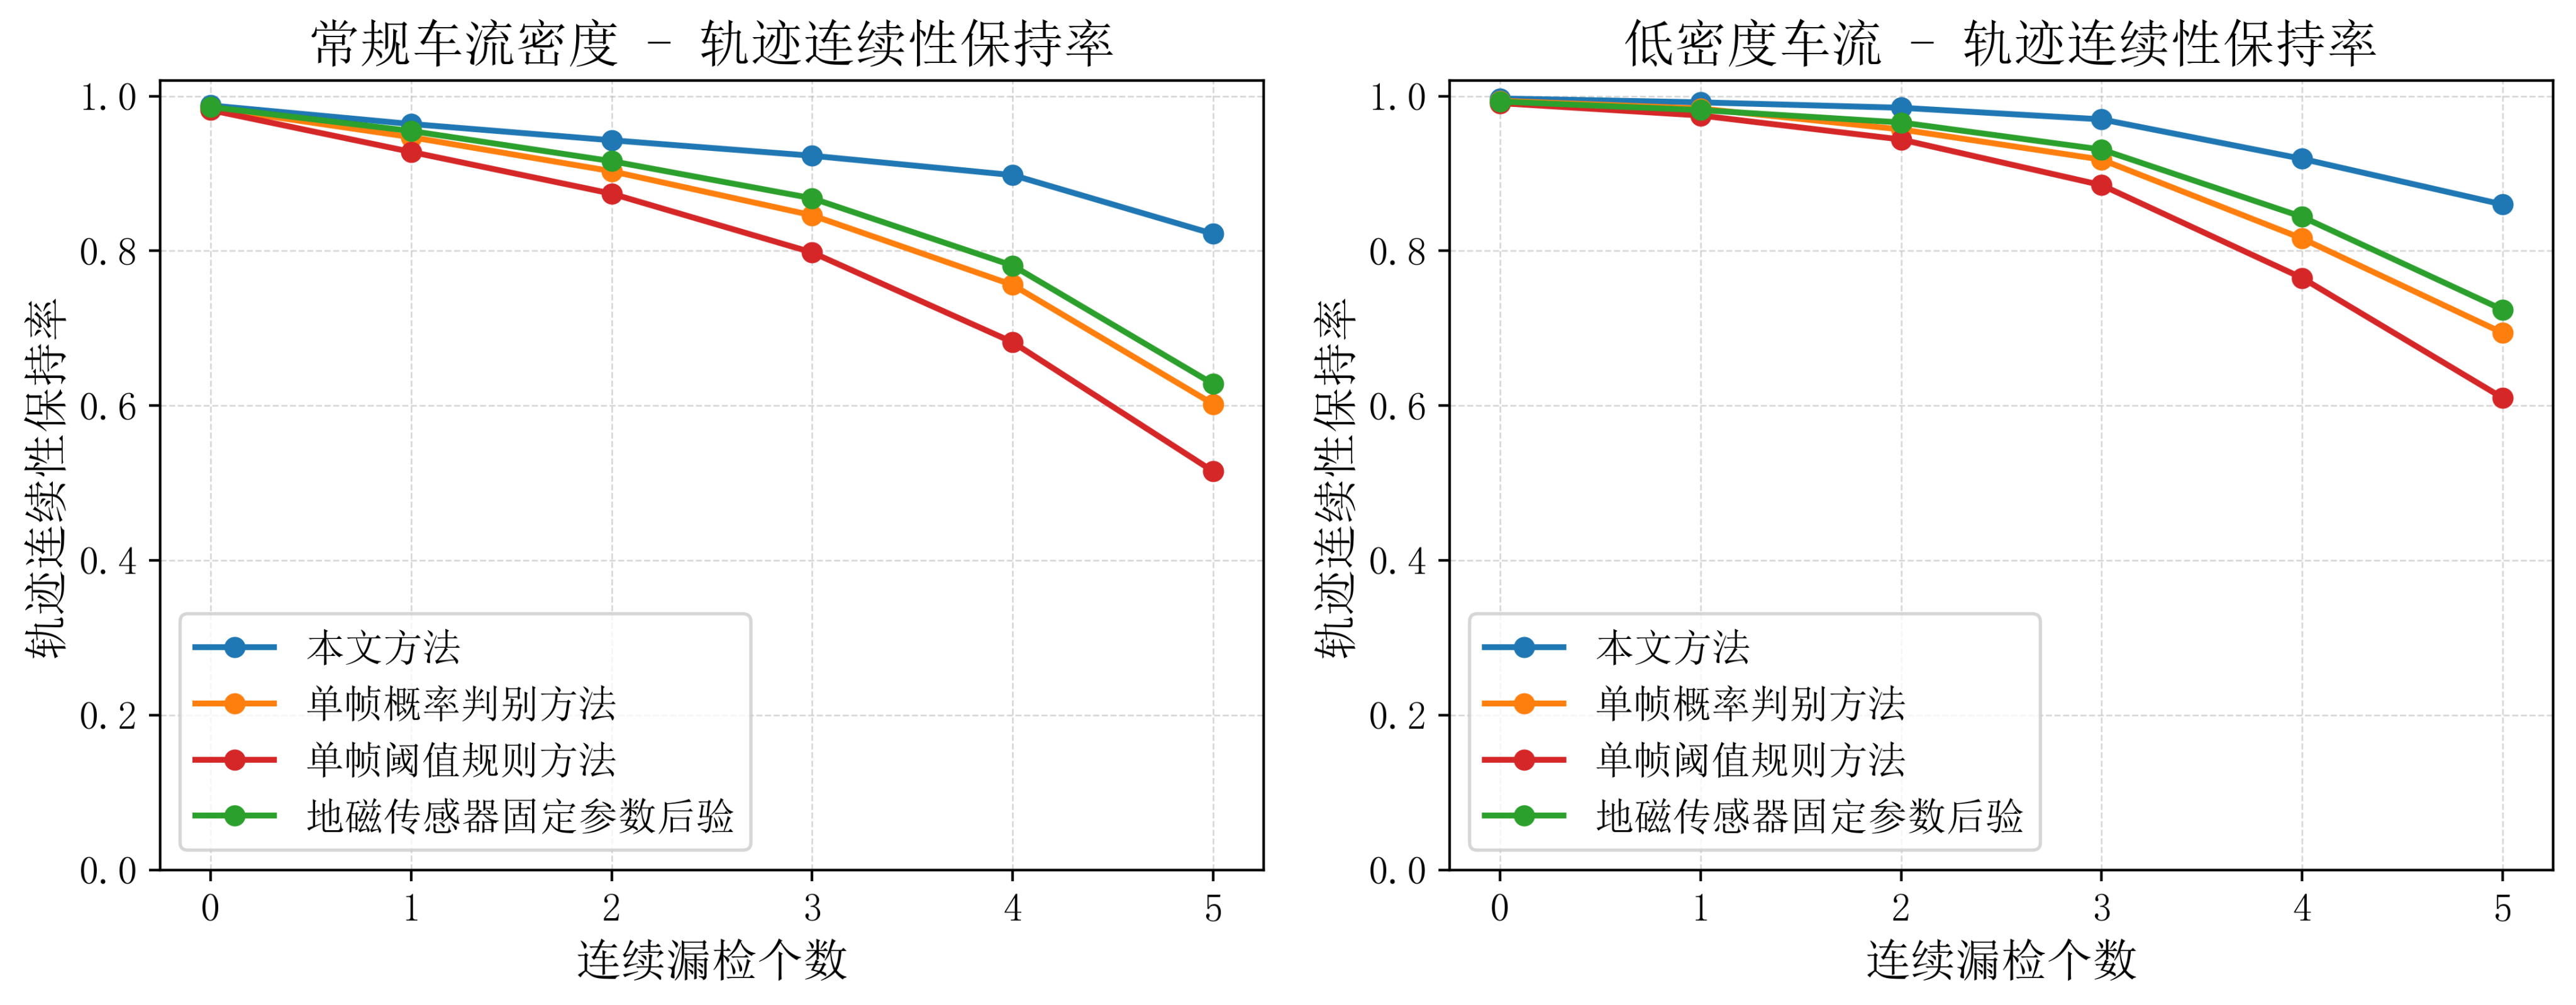
\includegraphics[width=0.95\textwidth]{code/chapter3/experiment1/exp1_results/3_11_1_continuity_v2.png}
	\caption{不同连续漏检长度下的轨迹连续保持率结果图}
	\label{fig:ch3_exp4_continuity}
\end{figure}

\begin{figure}[htbp]
	\centering
	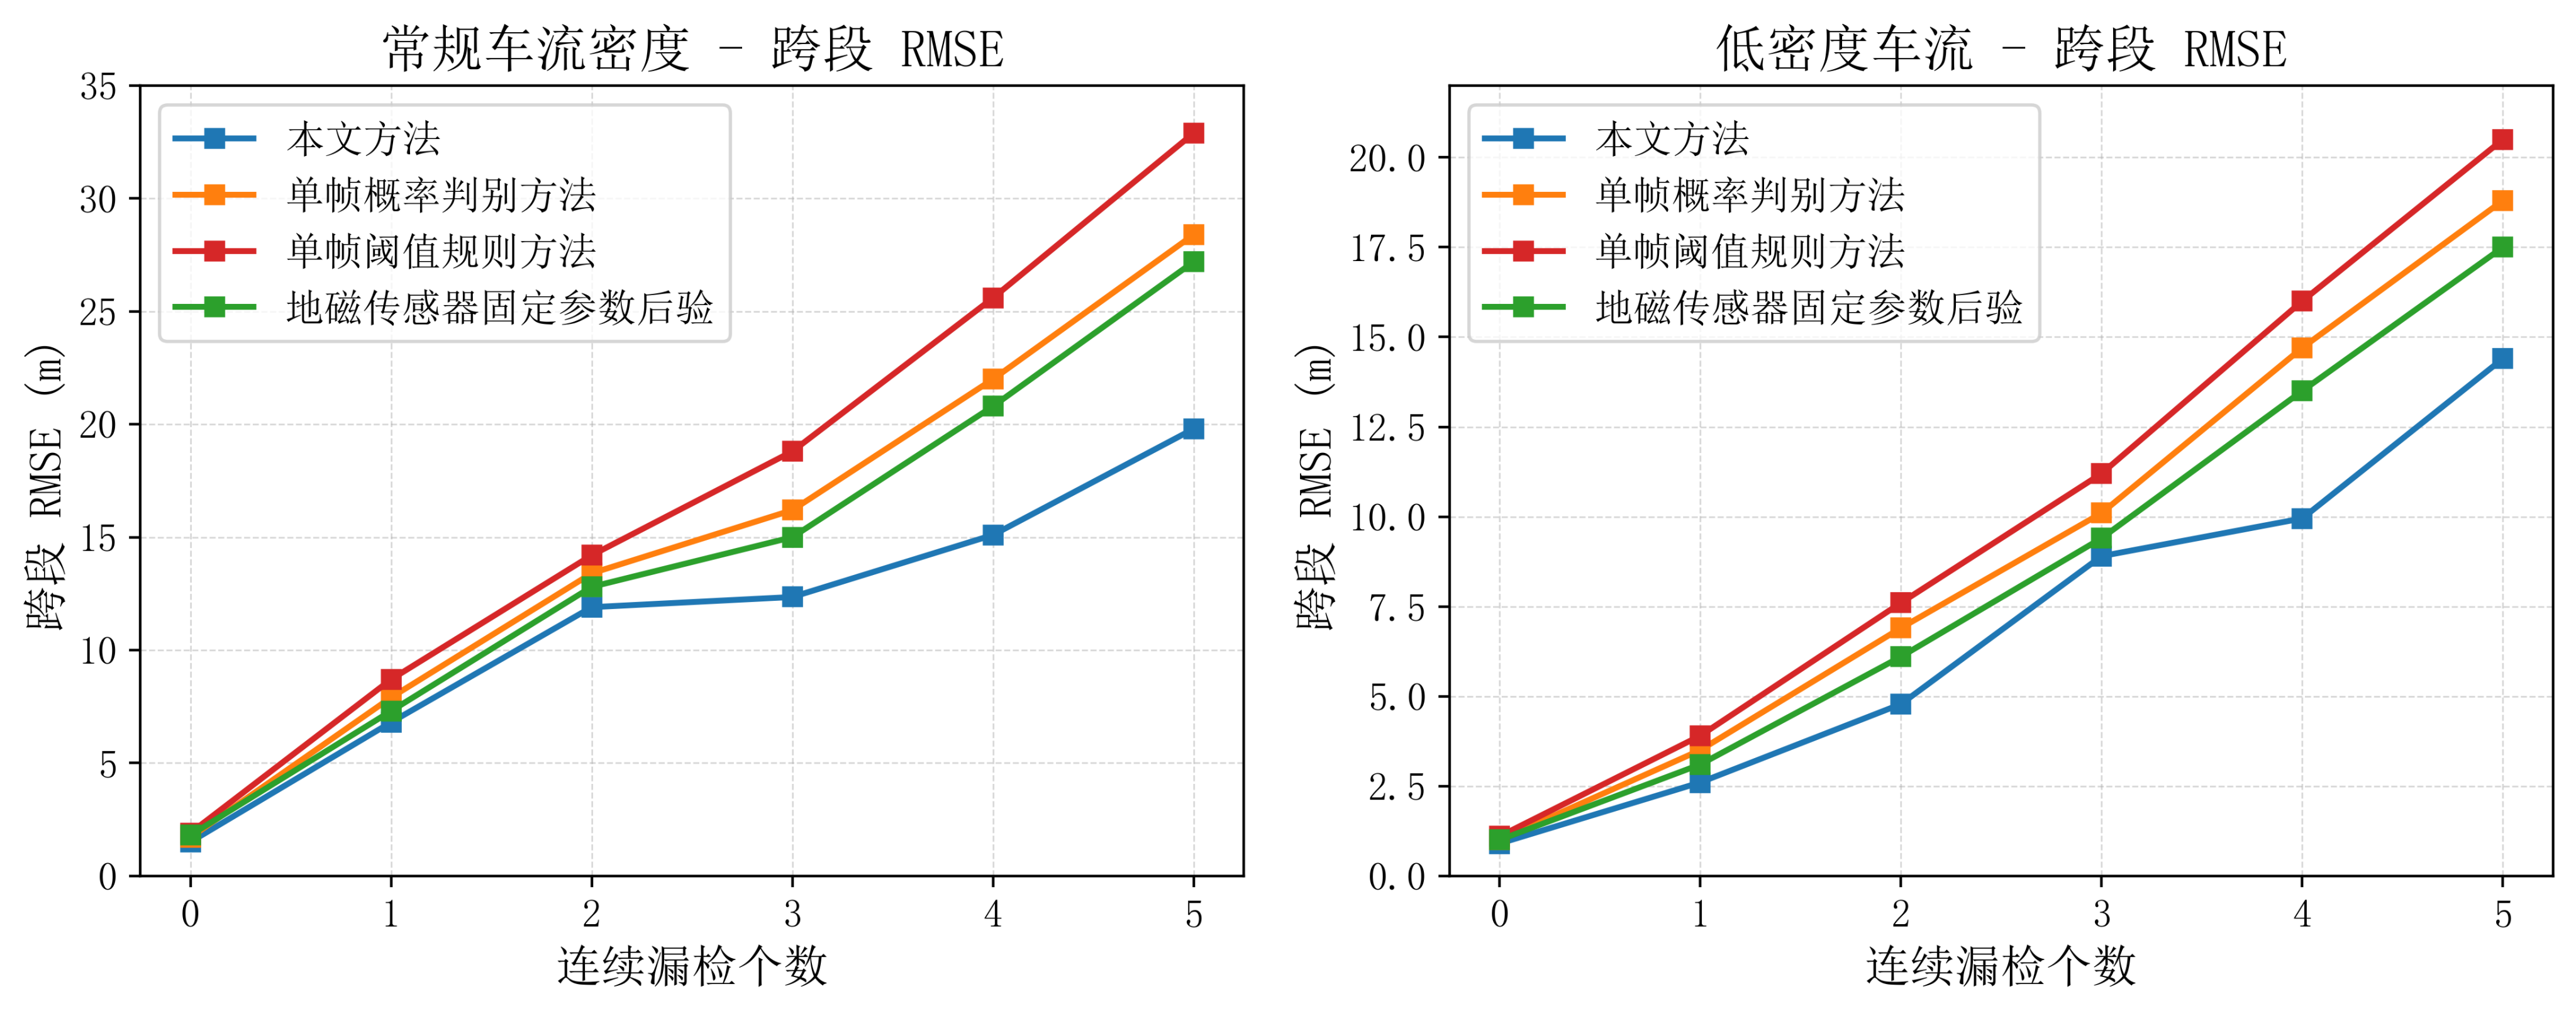
\includegraphics[width=0.95\textwidth]{code/chapter3/experiment1/exp1_results/3_11_2_rmse_v2.png}
	\caption{不同连续漏检长度下的跨段 RMSE 对比图}
	\label{fig:ch3_exp4_rmse}
\end{figure}

图~\ref{fig:ch3_exp4_continuity} 和图~\ref{fig:ch3_exp4_rmse} 表明，随着连续漏检长度增加，轨迹连续保持率整体下降，跨段位置均方根误差逐步增大。常规车流条件下，当 $m=2$ 至 $m=3$ 时，轨迹连续保持率仍维持在较高水平，而当 $m=4$ 时虽然连通性尚未明显崩溃，但跨段误差已经开始明显上升；当 $m=5$ 时，连通性和跨段精度均出现显著退化。低密度车流条件下，车辆时距较大，身份竞争相对较弱，因此轨迹连续保持率整体高于常规车流，并且对连续漏检的容忍范围更大。综合轨迹连续保持率、跨段位置误差以及辅助统计结果，可以将第三章方法的稳定容忍区间概括为：常规车流条件下连续 $2$ 至 $3$ 个地磁传感器漏检，低密度车流条件下连续 $3$ 至 $4$ 个地磁传感器漏检。超过该范围后，状态外推误差和身份歧义将共同加剧轨迹碎片化，这也为第四章面向长时缺测的片段级重构提供了直接的研究起点。

\section{本章小结}


本节围绕地磁传感器后验估计能力、邻道干扰与双车并行判别能力、连续漏检容忍范围、时间组织一致性以及各关键模块的独立贡献进行了系统验证。实验结果表明：地磁传感器状态自适应后验能够在地磁传感器退化与恢复过程中稳定跟踪检测概率和杂波强度变化；三状态场景递推显著降低了真实双车并行被误判为邻道干扰的比例，并有效抑制车道状态抖动；在常规车流条件下，本文方法可较稳定地容忍连续 2 至 3 个地磁传感器漏检，在低密度条件下该范围可扩展至连续 3 至 4 个地磁传感器；固定滞后回放能够明显提升迟到量测吸收比例以及在线处理结果与离线重排结果的一致率。消融实验进一步说明，地磁传感器状态自适应、三状态场景判别、磁特征一致性、软计数定稿更新以及固定滞后回放均对本章方法的最终性能具有独立而明确的贡献。上述结果不仅验证了本文方法的精度与鲁棒性，也明确了其适用边界，并为第四章面向长缺测工况的片段级在线聚类与轨迹重构提供了合理的输入条件与触发依据。


\chapter{长时缺测条件下基于在线聚类的轨迹片段重构算法}
\label{chap:cedas_fragment}

\graphicspath{
	{code/chapter4/experiment123/chapter4_results/exp1/}
	{code/chapter4/experiment123/chapter4_results/exp2/}
	{code/chapter4/experiment123/chapter4_results/exp3/}
}

\section{引言}

第三章给出的上游跟踪算法主要面向在线车辆目标跟踪，在量测时序矫正、状态估计、数据关联和轨迹管理的共同作用下，系统在一般工况下能够持续输出较为稳定的车辆轨迹。当漏检发生次数较少时，上游算法仍可借助局部时间一致性和运动约束维持轨迹连续性。但在系统长期运行过程中，若部分地磁传感器检测能力下降，连续缺测范围不断扩大，同一车辆可能在若干相邻观测位置上长期没有有效记录，原本连续的轨迹便会断裂为多个彼此独立的轨迹片段。此时，系统输出的主要问题不再是单次量测如何关联，而是这些已经分离的轨迹片段能否在后续处理阶段重新接续起来。针对这一问题，本章面向长时缺测条件，研究基于在线聚类的轨迹片段重构方法，以进一步提高车辆轨迹的连续性和身份一致性。

围绕这一目标，本章将长时缺测后的轨迹重构表述为一个面向样本流的在线聚类问题。首先，将上游算法输出的已经具有时空含义的轨迹片段以及少量未完成关联的单点量测统一表示为样本，并进一步介绍簇以及组织当前重构结果的簇图结构。在此基础上，本文设计面向簇最新状态，即簇尾的聚类相似度评分，完成样本归簇、新簇初始化、簇摘要更新和生命周期管理，使系统无需回到原始地磁检测数据重新执行跟踪，也能在样本持续到达的过程中逐步恢复同一车辆因长时缺测而断裂的轨迹。最后，通过实测数据上的可视化分析、整体效果对比、关键机制消融以及不同漏检强度下的实验结果，对所提方法的有效性进行验证。

\section{输入样本表示与簇图结构定义}

长时缺测后的轨迹重构首先要明确两个问题，首先是上游输出应如何统一表示，其次系统内部应如何组织已经归并的历史结果。前者决定后续相似度评分依赖的特征形式，后者决定历史信息能否在样本持续到达的条件下被稳定维护。基于这一点，下面先给出输入样本表示，再定义与之对应的簇图结构。

\subsection{输入样本表示}

为使轨迹片段和单点量测能够进入同一套在线归并流程，本文对输入数据采用统一的摘要式表示，只保留真正影响后续归簇判断的信息。设上游算法按时间输出的第 $m$ 个输入样本记为 $\mathbf{u}_m$，其统一表示为：
\begin{equation}
	\mathbf{u}_m=
	\left(
	\mathbf{q}_m,\,
	g_m,\,
	n_m,\,
	t_m^{\mathrm{s}},\,
	t_m^{\mathrm{e}}
	\right)
\end{equation}
其中，$\mathbf{q}_m$ 表示样本的方向向量，$g_m$ 表示样本的地磁代表值，$n_m$ 表示样本内有效观测数量，$t_m^{\mathrm{s}}$ 与 $t_m^{\mathrm{e}}$ 分别表示样本的起始时间戳和结束时间戳。这样定义以后，不同长度的轨迹片段以及退化的单点量测都可以先转换成同一种输入形式，再进入后续归簇流程。

在这些量中，$\mathbf{q}_m$ 是最关键的量。它用来概括样本在位置、车道和时间三维空间中的整体延伸方向。与将车道一致性单独拆成一项不同，本文直接把车道变化并入方向表示，使一个方向向量同时反映样本沿道路向前推进的趋势以及可能存在的车道变化。设样本起点和终点在纵向位置、车道和时间三维空间中的归一化差写为：
\begin{equation}
	\Delta \mathbf{r}_m=
	\begin{bmatrix}
		\dfrac{p_m^{\mathrm{e}}-p_m^{\mathrm{s}}}{D_p}\\[8pt]
		\dfrac{\ell_m^{\mathrm{e}}-\ell_m^{\mathrm{s}}}{D_{\ell}}\\[8pt]
		\dfrac{t_m^{\mathrm{e}}-t_m^{\mathrm{s}}}{D_t}
	\end{bmatrix}
\end{equation}
其中，$p_m^{\mathrm{s}}$ 与 $p_m^{\mathrm{e}}$ 分别为样本起点和终点的纵向位置，$\ell_m^{\mathrm{s}}$ 与 $\ell_m^{\mathrm{e}}$ 分别为样本起点和终点的车道取值，$D_p$、$D_{\ell}$ 与 $D_t$ 为三个维度的归一化尺度。则样本方向向量定义为：
\begin{equation}
	\mathbf{q}_m=
	\frac{\Delta \mathbf{r}_m}{\left\|\Delta \mathbf{r}_m\right\|_2+\varepsilon_q}
\end{equation}
其中，$\varepsilon_q$ 为稳定项。这样处理后，$\mathbf{q}_m$ 描述的是样本在三维时空中的整体延伸方向。当样本始终位于同一车道时，车道分量接近零；当样本伴随车道变化时，车道分量会自然反映到方向向量中。

地磁代表值 $g_m$ 用于在方向相近的候选关系之间提供辅助辨识信息。工程实现中，$g_m$ 可以取样本内部地磁峰值均值、归一化幅值均值或其他稳定的统计量，关键在于它能够较稳定地表征同一车辆样本之间的地磁相似性。支持度 $n_m$ 则表示该样本由多少有效观测支撑形成。一般而言，$n_m$ 越大，说明该样本越稳定，在后续簇尾摘要更新时也应占据更高权重。

当输入对象不是轨迹片段，而是上游算法未并入已有轨迹的单点量测时，仍将其视作退化样本统一处理。此时有：
\begin{equation}
	t_m^{\mathrm{s}}=t_m^{\mathrm{e}},\qquad n_m=1
\end{equation}
对于这类退化样本，其方向向量用道路主行驶方向初始化：
\begin{equation}
	\mathbf{q}_m=\mathbf{q}_{\mathrm{road}}
\end{equation}
其中，$\mathbf{q}_{\mathrm{road}}$ 为由道路几何结构和行驶方向给定的单位向量。经过这一处理，轨迹片段和单点量测就可以在统一样本定义下进入同一套在线归并流程。


\subsection{簇图结构定义}

有了统一的样本表示之后，还需要说明系统怎样保存已经归并的历史结果。由于本章处理的是持续到达的样本流，而不是一次性离线聚类，因此系统需要一种既能记录样本归并关系，又能快速支持下一次归簇判断的结构。为此，本文采用簇图结构组织当前的重构结果。

设当前系统中的簇集合记为：
\begin{equation}
	\mathbb{C}=\left\{C_1,C_2,\ldots,C_{N_C}\right\}
\end{equation}
其中，$C_c$ 表示第 $c$ 个簇，定义为：
\begin{equation}
	C_c=
	\left(
	\mathrm{Set}_c,\,
	\mathrm{Dir}_c,\,
	\mathcal{A}_c
	\right)
\end{equation}
其中，$\mathrm{Set}_c$ 为簇内样本集合，$\mathrm{Dir}_c$ 为样本之间的方向约束集合，$\mathcal{A}_c$ 为簇尾摘要。三者的作用是不同的。$\mathrm{Set}_c$ 保存已经归入该簇的全部样本，它代表这条候选重构轨迹当前已经收集到的证据；$\mathrm{Dir}_c$ 保存样本之间的方向约束，它代表哪些较晚到达的样本可以沿车辆真实运动方向接在较早样本之后；$\mathcal{A}_c$ 则是对簇当前尾端状态的压缩描述，它代表后续新样本归簇时真正参与比较的簇尾信息。这样定义以后，一个簇不再只是若干样本的简单堆积，而是一条按时间顺序向前延伸的候选重构轨迹。

若样本 $\mathbf{u}_m$ 被归入簇 $C_c$，则在簇内记作一个样本记录 $v_m\in\mathrm{Set}_c$。方向约束采用有序样本对表示。例如，若 $(v_a,v_b)\in\mathrm{Dir}_c$，则表示样本 $v_b$ 可以沿车辆行驶方向接在样本 $v_a$ 之后。这里的方向约束并不是为了引入复杂的图搜索，而是为了把样本之间的局部连接关系明确保存下来，使簇的增长过程始终沿时间顺序展开。可以将 $\mathrm{Set}_c$ 理解为这条候选轨迹已经收集到的全部样本，将 $\mathrm{Dir}_c$ 理解为这些样本之间谁先谁后的连接说明。

考虑到新样本归簇时主要与簇的尾端状态发生比较，本文将簇尾摘要定义为：
\begin{equation}
	\mathcal{A}_c=
	\left(
	\bar{\mathbf{q}}_c,\,
	\bar{g}_c,\,
	N_c,\,
	t_c^{\mathrm{tail}},\,
	E_c,\,
	s_c
	\right)
\end{equation}
其中，$\bar{\mathbf{q}}_c$ 为簇当前维护的代表方向向量，$\bar{g}_c$ 为簇当前维护的地磁代表值，$N_c$ 为簇累计支持度，$t_c^{\mathrm{tail}}$ 为簇尾端样本的结束时间，$E_c$ 为簇活跃度，$s_c\in\{\mathrm{active},\mathrm{closed}\}$ 为簇生命周期状态。上述量各自对应着明确的作用。$\bar{\mathbf{q}}_c$ 不是某一个具体样本的方向，而是簇尾近期整体延伸方向的代表，用来判断新样本是否还在沿着这条轨迹继续前进；$\bar{g}_c$ 不是某一次观测的瞬时地磁值，而是簇当前地磁水平的代表，用来在方向相近时进一步区分候选关系；$N_c$ 表示这个簇已经积累了多少支持信息，它直接影响后续摘要更新时历史样本和新样本的相对权重；$t_c^{\mathrm{tail}}$ 用于约束新旧样本的时间先后关系；$E_c$ 与 $s_c$ 则用于控制簇的活跃、关闭和输出。实际归簇时，系统并不会把新样本拿去和簇内所有历史样本逐一比较，而是优先与簇尾摘要比较。这样既保留了必要的历史信息，也控制了在线处理的计算开销。


\section{基于聚类相似度评分的在线聚类与簇管理算法}

在给出输入样本和簇图结构之后，后续问题就转化为一个明确的在线判定过程：新到达样本应接到哪一个已有簇的尾部，还是应当单独形成一个新簇。围绕这一问题，下面给出基于聚类相似度评分的在线聚类与簇管理算法。

\subsection{算法总体流程}

\begin{figure}[htbp]
	\centering
	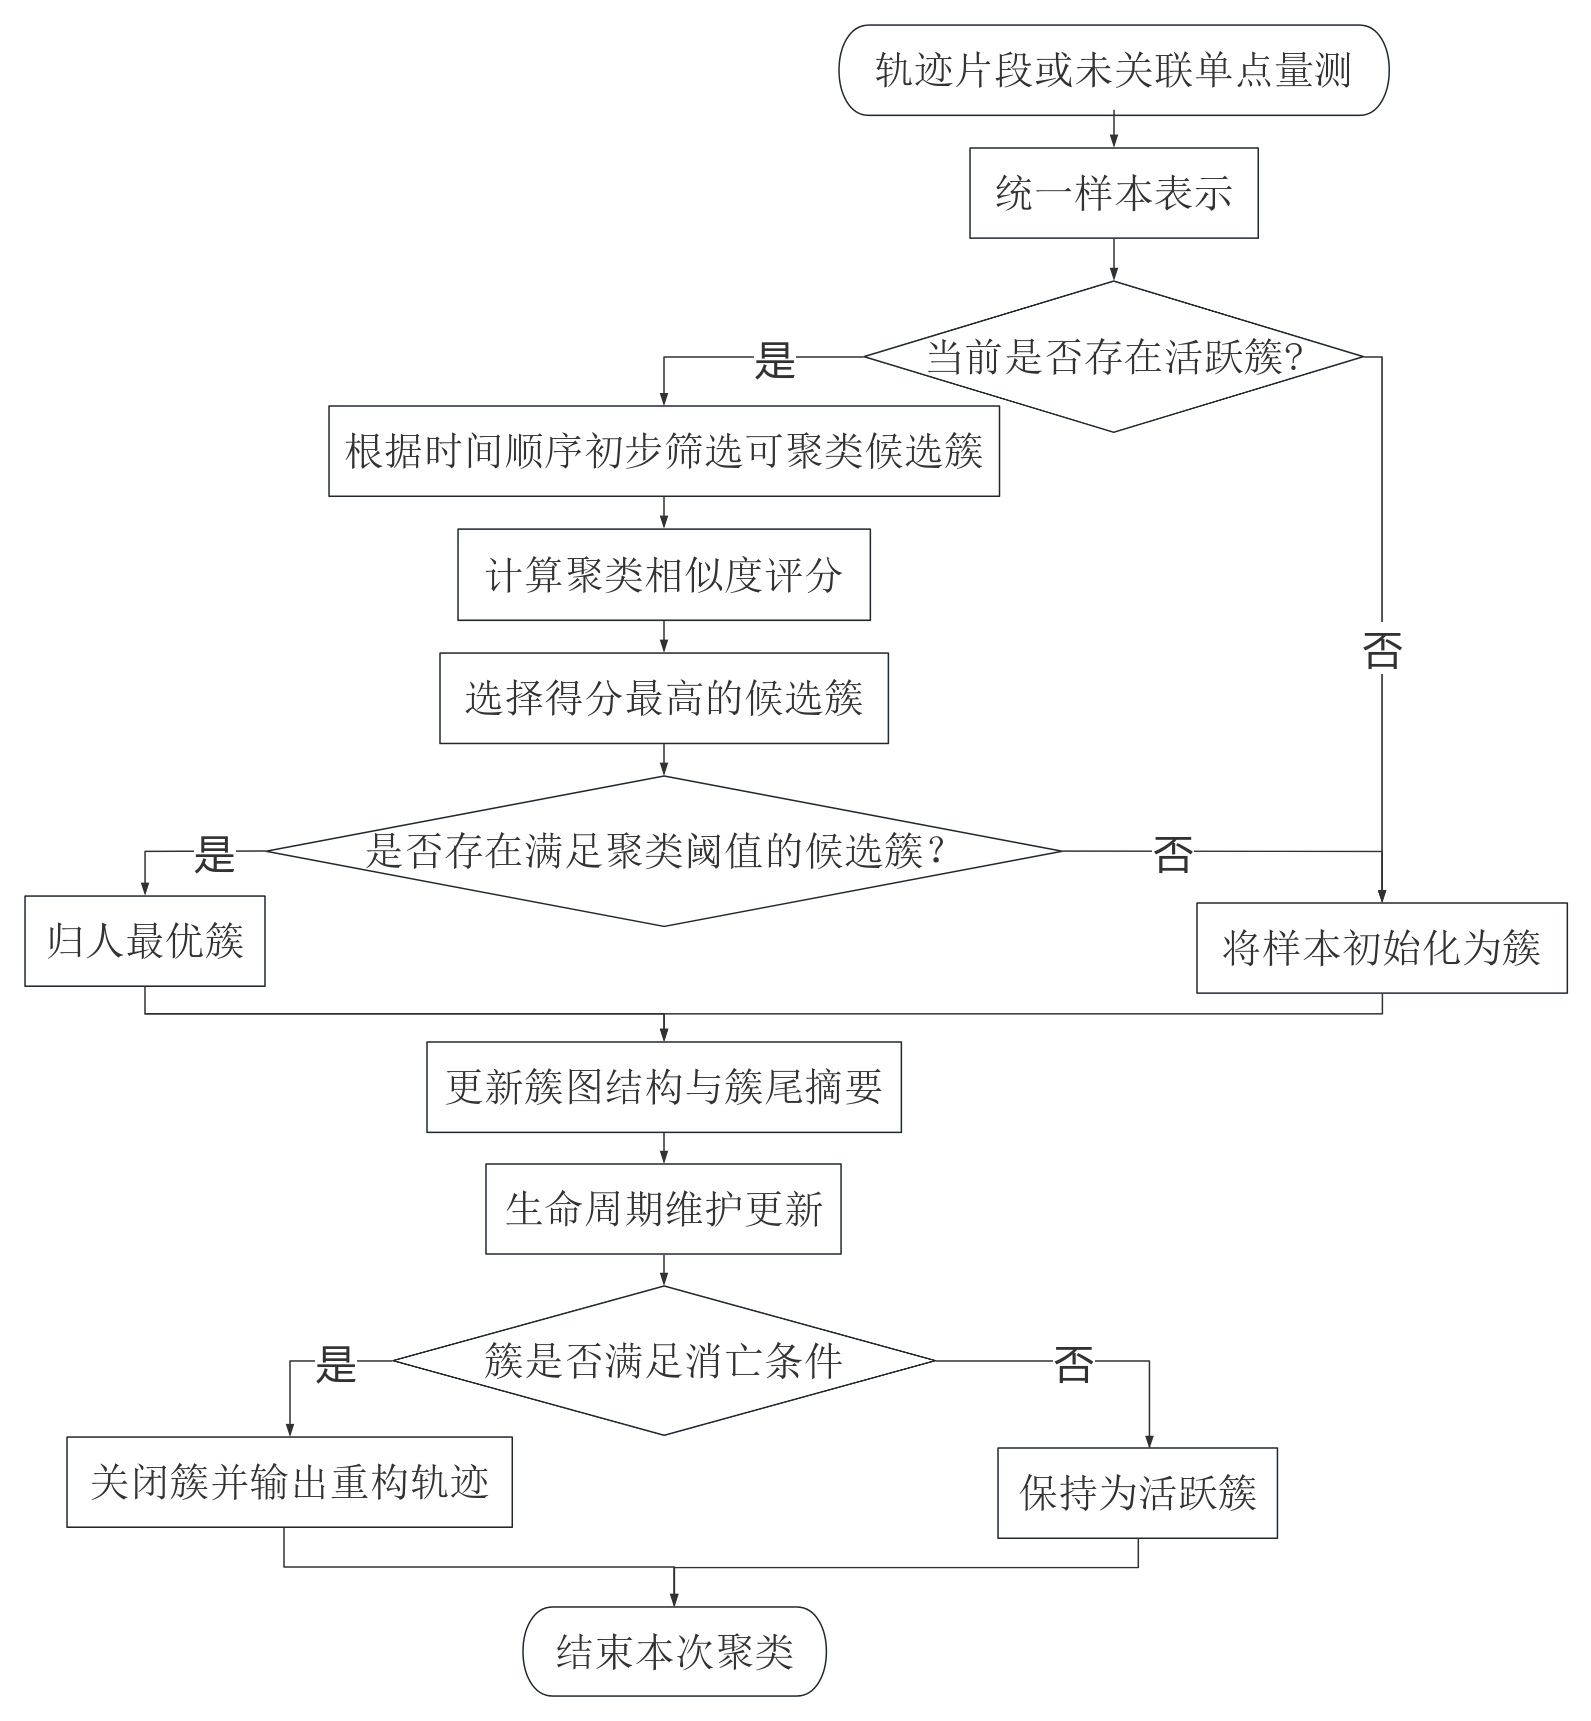
\includegraphics[width=0.82\textwidth]{images/chapter2/workflow.png}
	\caption{在线聚类与轨迹片段重构总体流程图}
	\label{fig:workflow}
\end{figure}

如图~\ref{fig:workflow}所示，系统按照样本到达顺序逐个执行在线归簇与轨迹重构。对于每个新到达样本，系统首先判断当前是否存在活跃簇。若当前不存在活跃簇，则直接以该样本初始化新簇；若当前存在活跃簇，则先依据时间顺序约束从活跃簇中筛选候选簇。若筛选后候选簇集合为空，同样以该样本初始化新簇。对于非空候选集合，系统进一步计算样本与各候选簇簇尾摘要之间的方向相似度和地磁相似度，并在时间顺序约束和方向约束共同作用下形成聚类相似度评分。得分最高者作为当前最优候选簇；若其评分达到聚类阈值，则将样本归入该簇，否则以该样本创建新簇。完成归簇后，系统同步更新簇中的样本集合、方向约束、簇尾摘要和生命周期状态。若某个簇在后续时段内满足关闭条件，则输出该簇对应的重构轨迹。整个过程始终面向样本流在线执行，不需要对全部历史轨迹片段重新离线聚类，因此既能保持重构结果的实时可用性，也便于把当前簇的状态继续用于后续样本判断。


\subsection{簇初始化}

当新到达样本无法与任何现有活跃簇形成可信连接时，系统以该样本为起点创建新簇。新簇主要完成三件事：记录第一个样本，建立空的方向约束集合，并用该样本初始化簇尾摘要。设新簇记为 $C_{\mathrm{new}}$，则有：
\begin{equation}
	\mathrm{Set}_{\mathrm{new}}=\{v_m\}
\end{equation}
\begin{equation}
	\mathrm{Dir}_{\mathrm{new}}=\varnothing
\end{equation}
\begin{equation}
	\mathcal{A}_{\mathrm{new}}=
	\left(
	\mathbf{q}_m,\,
	g_m,\,
	n_m,\,
	t_m^{\mathrm{e}},\,
	1,\,
	\mathrm{active}
	\right)
\end{equation}

这种初始化方式意味着，无论输入对象是一个长度较长的轨迹片段，还是只包含一次观测的退化样本，只要当前时刻没有足够证据将其并入已有簇，系统都会先保留它的独立性。这样做的好处是，每个新簇都从一个明确的时间起点开始生长，后续归并时也能直接利用其簇尾摘要参与判断。


\subsection{融合方向与地磁辅助的聚类相似度计算}

新样本到达后，系统首先不去比较所有已有簇，而是先筛掉明显不可能连接的对象。由于本章的归并方式是将后续样本接到已有簇的尾端，因此候选关系必须先满足时间顺序约束。记样本起始时间与簇尾结束时间之间的间隔为：
\begin{equation}
	\Delta t_{cm}=t_m^{\mathrm{s}}-t_c^{\mathrm{tail}}
\end{equation}
只有当新样本出现在簇尾之后，且间隔不超过允许的最大长缺测范围时，二者才有可能属于同一辆车。因此，候选簇集合定义为：
\begin{equation}
	\mathbb{C}_{\mathrm{cand}}(m)=
	\left\{
	C_c\in\mathbb{C}\ \middle|\ s_c=\mathrm{active},\ 0<\Delta t_{cm}\le T_{\max}
	\right\}
\end{equation}
其中，$T_{\max}$ 为允许拼接的最大时间间隔。该约束首先保证样本不会发生倒接，其次把明显间隔过长的簇排除在外，从而把后续比较集中在真正可能连接的少数候选簇上。若 $\mathbb{C}_{\mathrm{cand}}(m)$ 为空，则系统直接以当前样本初始化新簇，不再继续评分。

对于通过时间顺序初筛的候选簇，系统进一步检查方向是否一致。由于 $\mathbf{q}_m$ 与 $\bar{\mathbf{q}}_c$ 均为归一化向量，它们的内积可以直接反映方向接近程度。记方向约束函数为：
\begin{equation}
	g_{cm}^{\mathrm{dir}}=
	\mathbf{1}
	\left(
	\mathbf{q}_m^{\top}\bar{\mathbf{q}}_c\ge \tau_q
	\right)
\end{equation}
其中，$\tau_q$ 为方向约束阈值。若 $g_{cm}^{\mathrm{dir}}=0$，则说明新样本与该簇尾在整体延伸方向上明显不一致，应直接剔除。对通过方向约束的候选关系，方向相似度进一步定义为：
\begin{equation}
	S_{cm}^{\mathrm{dir}}=
	\frac{1+\mathbf{q}_m^{\top}\bar{\mathbf{q}}_c}{2}
\end{equation}
其中，$S_{cm}^{\mathrm{dir}}\in[0,1]$。当两者方向完全一致时，$S_{cm}^{\mathrm{dir}}$ 接近 $1$；当方向偏差增大时，该值相应减小。由于车道变化已经包含在方向向量的空间分量之中，因此这里不再额外设置独立的车道一致性评分项。这一步理解为，先判断两段样本是否大致朝同一方向延伸，再讨论它们是否足够相似。

仅靠方向信息仍然可能在多个方向接近的候选簇之间产生混淆，尤其是在同一路段存在多个相近轨迹片段时更是如此。为此，本文进一步引入地磁代表值相似度作为辅助约束。设样本与簇的地磁代表值分别为 $g_m$ 与 $\bar{g}_c$，则地磁相似度定义为：
\begin{equation}
	S_{cm}^{\mathrm{mag}}=
	\exp
	\left(
	-\frac{(g_m-\bar{g}_c)^2}{2\sigma_g^2+\varepsilon_g}
	\right)
\end{equation}
其中，$\sigma_g$ 为控制地磁相似度衰减速度的尺度参数，$\varepsilon_g$ 为稳定项。若二者地磁特征越接近，则 $S_{cm}^{\mathrm{mag}}$ 越接近 $1$；若二者差异明显，则该值相应减小。综合时间顺序约束、方向约束、方向相似度与地磁相似度，定义样本 $\mathbf{u}_m$ 与簇 $C_c$ 之间的聚类相似度评分为：
\begin{equation}
	\mathrm{Score}_{cm}=
	\mathbf{1}
	\left(
	0<\Delta t_{cm}\le T_{\max}
	\right)
	\cdot
	g_{cm}^{\mathrm{dir}}
	\cdot
	\left(
	w_q S_{cm}^{\mathrm{dir}}+w_g S_{cm}^{\mathrm{mag}}
	\right)
\end{equation}
其中，$w_q+w_g=1$，且 $w_q\ge 0$、$w_g\ge 0$。考虑到长时缺测后的轨迹重构首先依赖方向一致性，通常取 $w_q>w_g$，即方向项作为主导判据，地磁项主要负责在方向相近的候选关系之间进一步消歧。

对于候选簇集合中的各个簇，系统选取评分最高者作为当前样本的最优匹配簇：
\begin{equation}
	c^{\star}(m)=
	\arg\max_{C_c\in\mathbb{C}_{\mathrm{cand}}(m)}\mathrm{Score}_{cm}
\end{equation}
当最优候选簇评分满足：
\begin{equation}
	\mathrm{Score}_{c^{\star}(m),m}\ge \tau_{\mathrm{clus}}
\end{equation}
则将样本 $\mathbf{u}_m$ 归入簇 $C_{c^{\star}(m)}$；否则，以该样本初始化新簇。至此，样本归簇判定被统一表述为一个面向簇尾的在线评分过程。整个过程可以概括为先按时间顺序筛选候选簇，再用方向约束排除明显不合理的连接，最后用地磁相似度在少数方向相近的候选簇之间做进一步区分。这样处理既符合车辆沿道路单向推进的物理规律，也保持了在线实现所需的计算简洁性。


\subsection{簇更新与生命周期管理}

当样本 $\mathbf{u}_m$ 被归入已有簇 $C_c$ 后，系统需要同步完成簇结构更新、簇尾摘要更新以及生命周期维护。三者分别对应保存新旧样本连接关系、刷新簇当前代表状态以及控制簇是否继续保留。

首先，在簇结构层面，需要完成样本集合和方向约束集合的更新：
\begin{equation}
	\mathrm{Set}_c\leftarrow \mathrm{Set}_c\cup\{v_m\}
\end{equation}
\begin{equation}
	\mathrm{Dir}_c\leftarrow \mathrm{Dir}_c\cup\{(v_{\mathrm{tail}},v_m)\}
\end{equation}
其中，$v_{\mathrm{tail}}$ 表示更新前簇的尾端样本。上述方向约束表示新样本 $v_m$ 可以沿车辆行驶方向接在原簇尾样本之后。这一步的作用不是为了构造复杂图，而是为了把样本之间的先后连接关系明确保存下来，使簇在结构上始终保持为一条按时间顺序向前延伸的样本链。

其次，在簇尾摘要层面，本文采用支持度加权的方式更新簇的代表方向和地磁代表值。设并入前簇的累计支持度为 $N_c$，当前样本支持度为 $n_m$，则更新后的簇代表方向向量和地磁代表值分别为：
\begin{equation}
	\bar{\mathbf{q}}_c^{+}=
	\frac{
		N_c\bar{\mathbf{q}}_c+n_m\mathbf{q}_m
	}{
		\left\|
		N_c\bar{\mathbf{q}}_c+n_m\mathbf{q}_m
		\right\|_2+\varepsilon_q
	}
\end{equation}
\begin{equation}
	\bar{g}_c^{+}=
	\frac{N_c\bar{g}_c+n_m g_m}{N_c+n_m}
\end{equation}
随后更新簇尾摘要中的相关量：
\begin{equation}
	\bar{\mathbf{q}}_c\leftarrow \bar{\mathbf{q}}_c^{+}
\end{equation}
\begin{equation}
	\bar{g}_c\leftarrow \bar{g}_c^{+}
\end{equation}
\begin{equation}
	N_c\leftarrow N_c+n_m
\end{equation}
\begin{equation}
	t_c^{\mathrm{tail}}\leftarrow t_m^{\mathrm{e}}
\end{equation}
这种更新方式使支持度较大的稳定样本在摘要更新时占据更高权重，而支持度较小的退化样本不会对已有簇的主方向和地磁代表值造成过度扰动。与简单覆盖相比，支持度加权更新更能反映簇在持续生长过程中的整体趋势，也更有利于保持簇尾摘要的稳定性。

最后，在生命周期管理方面，本文为每个簇维护活跃度 $E_c$，以控制系统在长期运行中的簇数量。设当前处理时刻为 $t$，则簇活跃度的时间衰减写为：
\begin{equation}
	E_c(t)=E_c(t_c^{\mathrm{tail}})
	\exp
	\left(
	-\frac{t-t_c^{\mathrm{tail}}}{\tau_E}
	\right)
\end{equation}
其中，$\tau_E$ 为活跃度衰减时间常数。当样本 $\mathbf{u}_m$ 成功归入簇 $C_c$ 后，执行：
\begin{equation}
	E_c\leftarrow
	\min
	\left(
	1,\,
	E_c+\alpha_E\cdot \min\left(1,\frac{n_m}{n_{\mathrm{ref}}}\right)
	\right)
\end{equation}
\begin{equation}
	s_c\leftarrow \mathrm{active}
\end{equation}
其中，$\alpha_E$ 为活跃度增益系数，$n_{\mathrm{ref}}$ 为支持度归一化参考值。反之，若某个簇在较长时间内未再吸收新样本，并且同时满足 $E_c<E_{\min}$ 与 $t-t_c^{\mathrm{tail}}>T_{\mathrm{del}}$，则将其状态置为：
\begin{equation}
	s_c\leftarrow \mathrm{closed}
\end{equation}
当一个簇被关闭后，说明它在当前时间范围内已经完成生长。此时，簇结构中按时间顺序组织的样本链即可作为该车辆在长时缺测条件下的重构轨迹输出。由此可见，所提方法本质上是一个面向样本流的在线增量归并过程。其中，时间顺序约束用于防止样本倒接，方向约束提供主要判据，地磁代表值负责辅助消歧，簇尾摘要使历史信息能够以压缩形式持续参与当前决策，而生命周期管理则保证系统在长期运行时保持可控的簇规模。

\section{实验与结果分析}

\subsection{实验数据采集}

实验采用东乡西高速公路实测数据。该路段为单向双车道场景，有效监测长度约为 $1080\,\mathrm{m}$。沿道路两侧车道线共布设 $144$ 个地磁传感器，相邻地磁传感器间距为 $15\,\mathrm{m}$，同时设置路侧监控摄像机，用于对车辆实际通行过程进行人工核验和结果对照。东乡西路段的监测场景与数据采集方式如图~\ref{fig:ch4_dxx_monitor} 所示，相关部署配置见表~\ref{tab:ch4_data_config}。

\begin{figure}[htbp]
	\centering
	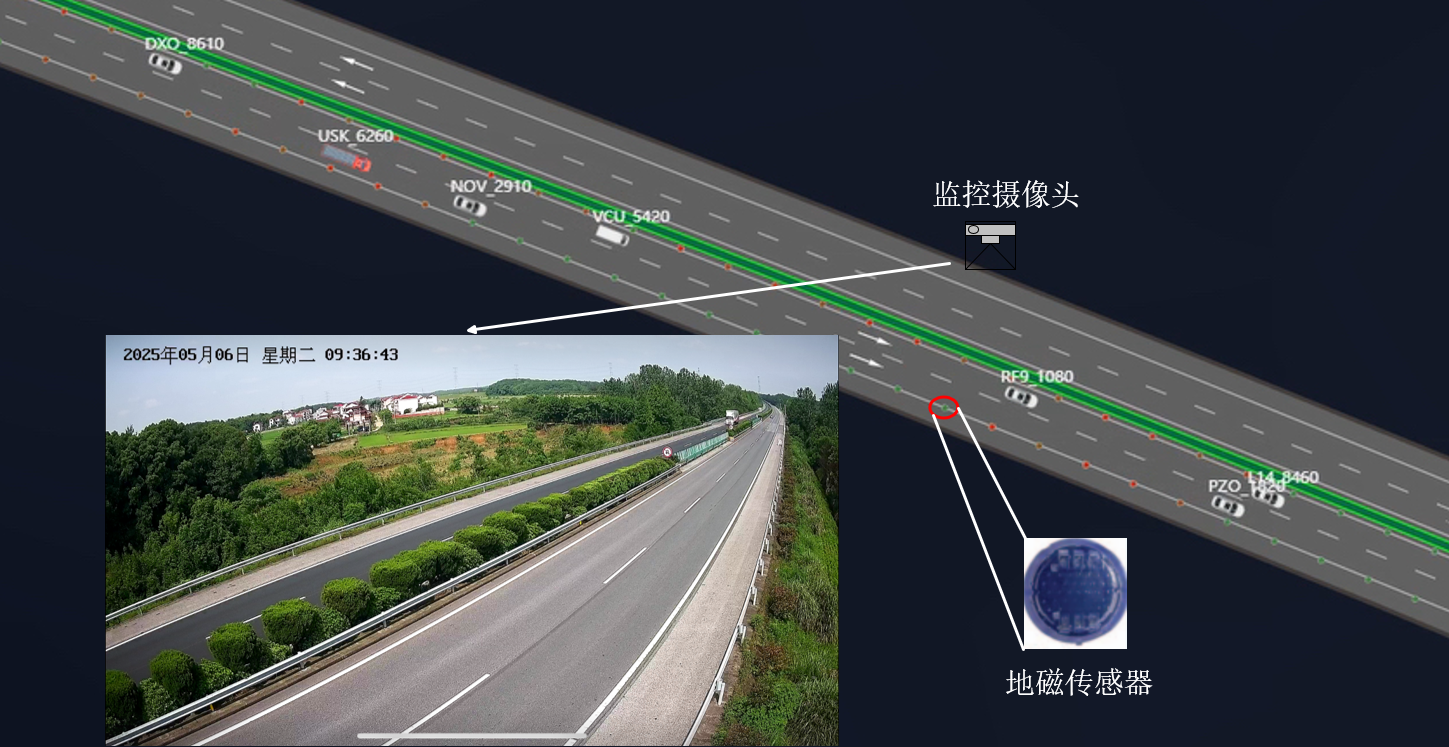
\includegraphics[width=0.82\textwidth]{images/chapter2/DXXsystem.png}
	\caption{东乡西路段监测场景与数据采集示意图}
	\label{fig:ch4_dxx_monitor}
\end{figure}

\begin{table}[htbp]
	\centering
	\caption{东乡西路段数据采集与部署配置}
	\label{tab:ch4_data_config}
	\renewcommand{\arraystretch}{1.2}
	\begin{tabular}{p{0.26\textwidth}p{0.62\textwidth}}
		\toprule
		项目 & 配置说明 \\
		\midrule
		实测路段 & 江西省东乡西高速公路单向双车道路段 \\
		监测长度 & 约 $1080\,\mathrm{m}$ \\
		地磁传感器数量 & $144$ 个地磁传感器，沿两侧车道线成对布设 \\
		地磁传感器间距 & $15\,\mathrm{m}$ \\
		辅助核验设备 & 路侧监控摄像机，用于车辆通行过程核验与标签校对 \\
		原始上报内容 & 触发时间、地磁传感器编号、峰值地磁扰动、车道标识、持续时间及入队时间等字段 \\
		\bottomrule
	\end{tabular}
\end{table}

实测系统以连续上报记录的形式接收车辆通过信息，每条原始记录至少包含触发时间、数据入队时间、地磁传感器编号、峰值地磁扰动和车道标识等内容。本章并不直接对这些原始记录进行聚类，而是先由上游算法完成量测时序矫正、状态估计和数据关联，再将输出的轨迹片段及未并入轨迹的单点量测作为重构输入。本章实验关注的重点也集中在长时缺测条件下的轨迹片段重构能力。

在系统工作年限过久后，地磁传感器的上报率会出现较大降低。表~\ref{tab:ch4_reporting_status} 给出了三个代表性观测时段的统计结果。可以看到，地磁传感器不上报率最高达到 $50.7\%$，最大连续不上报数量达到 $5$ 个地磁传感器。这意味着真实道路中不仅会出现随机单点漏检，还会出现跨多个相邻地磁传感器的连续缺测，上游输出也会因此断裂为多个彼此分离的轨迹片段，这正是本章要处理的情况。为避免参数选择与性能评估相互耦合，本本文先从实测数据中随机选取 $20\,\mathrm{min}$ 原始序列，并结合监控视频完成车辆标签人工标定与核验，用于算法参数标定；在此基础上，再选取一段长度为 $25\,\mathrm{min}$ 的独立实测序列，同样结合监控视频完成车辆标签人工标定与核验，作为主测评集，该序列共包含 $256$ 辆车辆。后续各方法均基于同一批上游输出样本进行处理，并保持一致的样本到达顺序。为了进一步考察不同长缺测强度下的稳定性，后续实验还将在此基础上构造不同总体漏检率 $\eta_{\mathrm{miss}}$ 与最大连续缺测长度 $L_{\mathrm{miss}}$ 的组合场景。

\begin{table}[htbp]
	\centering
	\caption{代表性观测时段的地磁传感器不上报情况}
	\label{tab:ch4_reporting_status}
	\begin{tabular}{lccc}
		\toprule
		统计日期 & 2024.12.15 & 2024.12.16 & 2025.02.27 \\
		\midrule
		地磁传感器不上报率 & 50.7\% & 31.9\% & 33.3\% \\
		最大连续不上报数量 & 5 & 5 & 4 \\
		\bottomrule
	\end{tabular}
\end{table}

\subsection{评价指标}

本章实验重点关注已经碎片化的样本能否被重新归并为属于同一车辆的完整轨迹，以及在归并过程中是否发生错误合并。因此，后续主要从片段连接是否正确、错误合并是否增多、碎片数量是否减少以及最终分组是否与真实轨迹一致四个方面进行评价。具体采用的指标包括片段拼接精确率 $P_{\mathrm{link}}$、片段拼接召回率 $R_{\mathrm{link}}$、片段拼接 $F1$ 值 $F1_{\mathrm{link}}$、错并率 $R_{\mathrm{wm}}$、碎片消减量 $\mathrm{Frag}_{\mathrm{drop}}$ 和聚类一致性指标 $\mathrm{FMI}$。

设上游算法输出并进入本章重构流程的样本集合为：
\begin{equation}
	\mathcal{U}=\left\{\mathbf{u}_1,\mathbf{u}_2,\ldots,\mathbf{u}_M\right\}
\end{equation}
其中，$\mathbf{u}_m$ 可以是轨迹片段，也可以是未被上游算法并入轨迹的单点量测。根据人工标注或参考轨迹，可得到真实可拼接关系集合 $\mathcal{L}^{\mathrm{gt}}$。若 $\left(\mathbf{u}_i,\mathbf{u}_j\right)\in\mathcal{L}^{\mathrm{gt}}$，则表示二者属于同一真实车辆，且在时间顺序上应连接为同一条轨迹。相应地，算法输出的预测拼接关系集合记为 $\mathcal{L}^{\mathrm{pred}}$。据此，定义真正例、假正例和假反例如下：
\begin{equation}
	N_{\mathrm{TP}}=\left|\mathcal{L}^{\mathrm{gt}}\cap\mathcal{L}^{\mathrm{pred}}\right|
\end{equation}
\begin{equation}
	N_{\mathrm{FP}}=\left|\mathcal{L}^{\mathrm{pred}}\setminus\mathcal{L}^{\mathrm{gt}}\right|
\end{equation}
\begin{equation}
	N_{\mathrm{FN}}=\left|\mathcal{L}^{\mathrm{gt}}\setminus\mathcal{L}^{\mathrm{pred}}\right|
\end{equation}

由此得到片段拼接精确率、片段拼接召回率和片段拼接 $F1$ 值：
\begin{equation}
	P_{\mathrm{link}}
	=
	\frac{N_{\mathrm{TP}}}{N_{\mathrm{TP}}+N_{\mathrm{FP}}}
\end{equation}
\begin{equation}
	R_{\mathrm{link}}
	=
	\frac{N_{\mathrm{TP}}}{N_{\mathrm{TP}}+N_{\mathrm{FN}}}
\end{equation}
\begin{equation}
	F1_{\mathrm{link}}
	=
	\frac{2P_{\mathrm{link}}R_{\mathrm{link}}}{P_{\mathrm{link}}+R_{\mathrm{link}}}
\end{equation}
其中，$P_{\mathrm{link}}$ 反映算法给出的片段连接中有多少是真实正确的，$R_{\mathrm{link}}$ 反映真实应恢复的连接中有多少被成功找回，$F1_{\mathrm{link}}$ 则综合刻画重构结果在正确性和完整性之间的平衡，因此作为本章的主评价指标。

为更直接地反映错误合并风险，定义错并率为：
\begin{equation}
	R_{\mathrm{wm}}
	=
	\frac{N_{\mathrm{FP}}}{N_{\mathrm{TP}}+N_{\mathrm{FP}}}
\end{equation}
设重构前片段总数为 $\mathrm{Frag}_{\mathrm{before}}$，重构后输出轨迹数为 $\mathrm{Frag}_{\mathrm{after}}$，则碎片消减量定义为：
\begin{equation}
	\mathrm{Frag}_{\mathrm{drop}}
	=
	\mathrm{Frag}_{\mathrm{before}}-\mathrm{Frag}_{\mathrm{after}}
\end{equation}
其中，$R_{\mathrm{wm}}$ 越小，说明不同车辆的样本越不容易被误并到同一条轨迹中；$\mathrm{Frag}_{\mathrm{drop}}$ 越大，说明重构后碎片化程度缓解得越明显。不过，碎片数减少并不必然意味着重构结果更好，因此该指标需要与 $F1_{\mathrm{link}}$ 和 $R_{\mathrm{wm}}$ 结合分析。

为了从整体分组层面评价重构结果与真实轨迹之间的一致性，本文采用 Fowlkes Mallows 指数 $\mathrm{FMI}$。设真实分组和预测分组分别为：
\begin{equation}
	\mathcal{C}
	=
	\left\{C_1,C_2,\ldots,C_K\right\}
\end{equation}
\begin{equation}
	\hat{\mathcal{C}}
	=
	\left\{\hat{C}_1,\hat{C}_2,\ldots,\hat{C}_S\right\}
\end{equation}
对于任意样本对 $\left(\mathbf{u}_i,\mathbf{u}_j\right)$，其中 $i<j$，记 $a$ 为在真实分组与预测分组中均被划入同一类的样本对数量，$b$ 为在真实分组中属于同一类但在预测分组中被分开的样本对数量，$c$ 为在真实分组中属于不同类但在预测分组中被错误归为同一类的样本对数量，则 $\mathrm{FMI}$ 定义为：
\begin{equation}
	\mathrm{FMI}
	=
	\sqrt{
		\frac{a}{a+b}
		\cdot
		\frac{a}{a+c}
	}
\end{equation}
$\mathrm{FMI}$ 越接近 $1$，说明最终输出的整体聚类结构越接近真实车辆分组。为便于后续结果分析，表~\ref{tab:ch4_metric_summary} 总结了各指标的含义及优化方向。后续分析将以 $F1_{\mathrm{link}}$ 为主，并结合 $R_{\mathrm{wm}}$、$\mathrm{Frag}_{\mathrm{drop}}$ 和 $\mathrm{FMI}$ 对方法性能进行综合判断。

\begin{table}[htbp]
	\centering
	\caption{第四章评价指标及含义}
	\label{tab:ch4_metric_summary}
	\renewcommand{\arraystretch}{1.2}
	\begin{tabular}{p{0.19\textwidth}p{0.56\textwidth}c}
		\toprule
		指标 & 主要含义 & 优化方向 \\
		\midrule
		$P_{\mathrm{link}}$ & 预测拼接关系中真实正确连接所占比例，反映重构结果的准确性 & 越大越好 \\
		$R_{\mathrm{link}}$ & 真实应恢复的连接关系中被成功找回的比例，反映重构完整性 & 越大越好 \\
		$F1_{\mathrm{link}}$ & 综合平衡片段拼接精确率与召回率，是本章主评价指标 & 越大越好 \\
		$R_{\mathrm{wm}}$ & 所有已执行拼接中错误拼接所占比例，反映误并风险 & 越小越好 \\
		$\mathrm{Frag}_{\mathrm{drop}}$ & 重构前后轨迹碎片数的减少量，反映碎片化缓解程度 & 越大越好 \\
		$\mathrm{FMI}$ & 预测聚类结构与真实轨迹分组之间的一致性程度 & 越大越好 \\
		\bottomrule
	\end{tabular}
\end{table}

\subsection{整体重构效果可视化分析}

图~\ref{fig:4_2_typical_case} 给出了主场景下的在线聚类结果可视化。为便于观察重构效果，图中以样本的归一化位置、车道信息和归一化时间作为三维坐标，不同颜色表示最终归属的不同轨迹簇。可以看到，大多数样本能够沿车辆实际行驶方向形成连续且相互分离的簇结构，说明所提方法能够把长时缺测后被切断的短片段重新组织为较完整的轨迹。对于局部位置接近、时间相邻、甚至存在一定交叠趋势的样本，图中仍保持了较好的簇间区分度，未出现大范围混簇现象。这说明时间顺序约束、方向约束以及地磁辅助信息在样本接续过程中确实发挥了作用，能够在仅依赖位置邻近关系容易混淆的区域提供额外判别依据。

\begin{figure}[htbp]
	\centering
	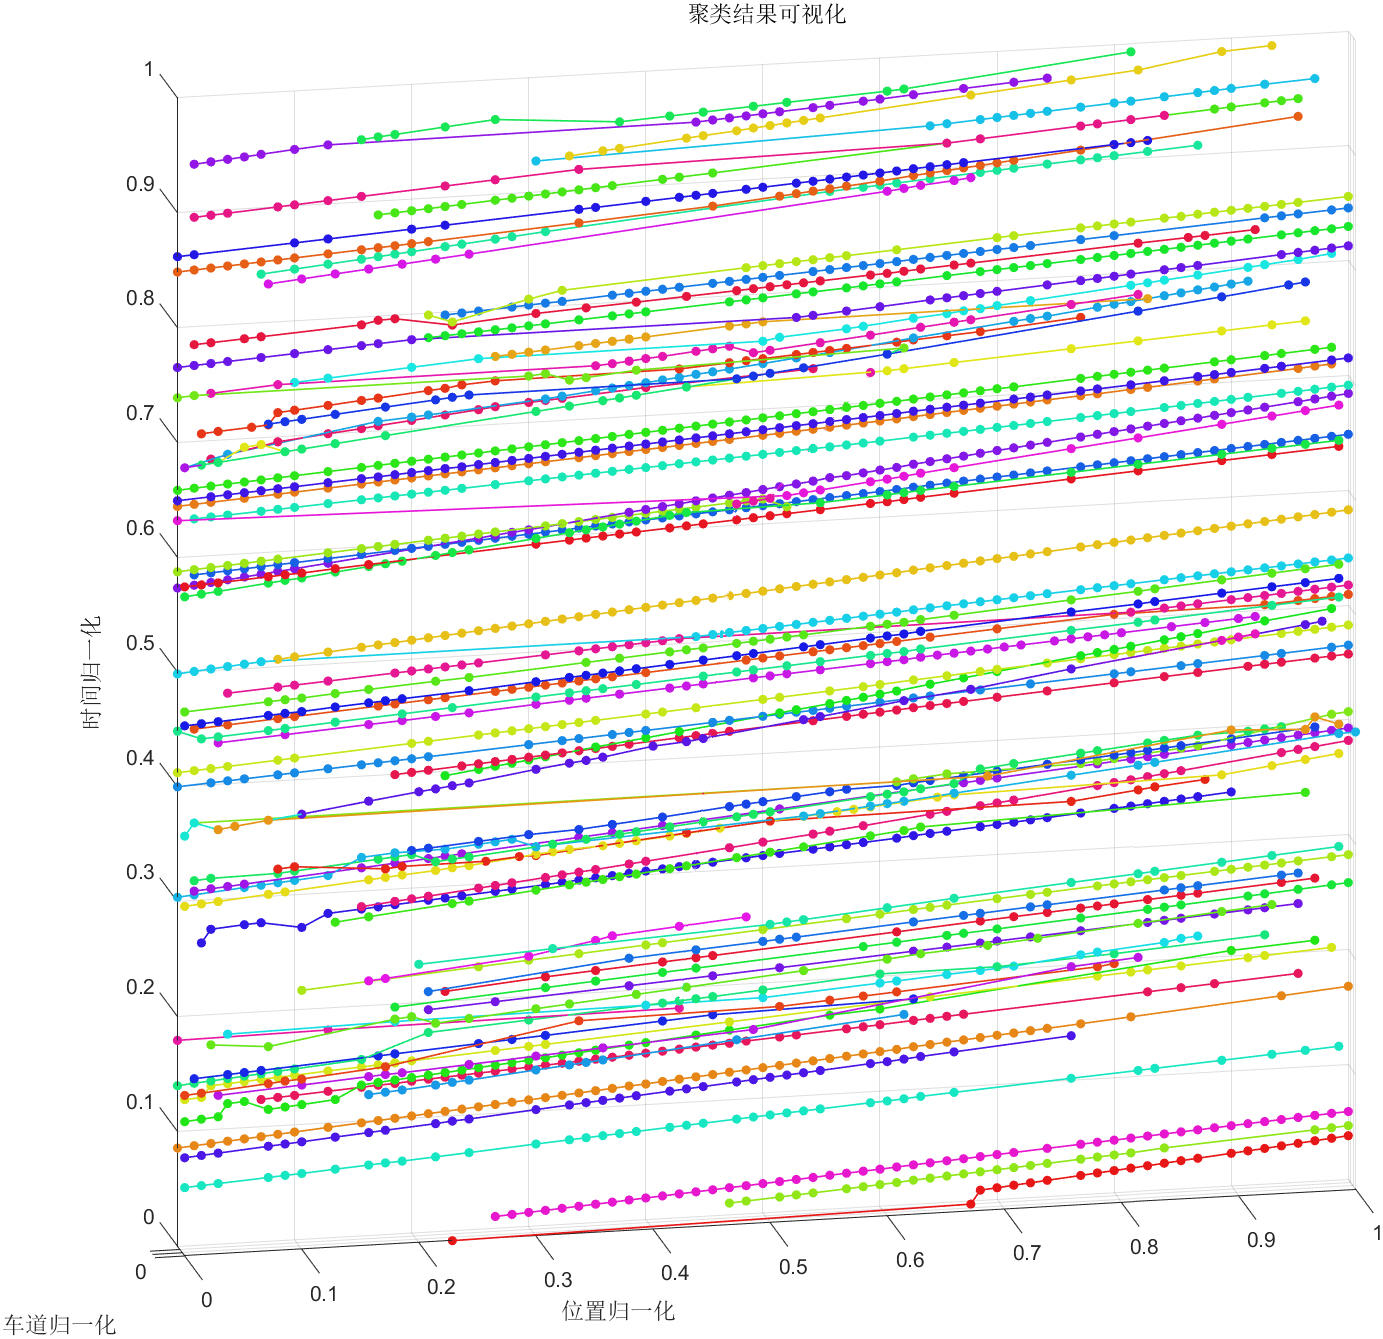
\includegraphics[width=0.72\textwidth]{images/chapter2/cluster_result.jpg}
	\caption{在线聚类结果可视化结果图}
	\label{fig:4_2_typical_case}
\end{figure}

图~\ref{fig:4_3_length_distribution} 进一步给出了重构前后轨迹长度分布的变化。重构前，轨迹长度主要集中在较短区间，说明上游输出仍然具有明显的碎片化特征；重构后，长度分布整体向中长轨迹区间移动，短片段数量明显减少，中等长度和较长长度轨迹占比有所提升。这表明所提方法确实恢复了一部分原本属于同一车辆的断裂片段。与此同时，分布并未出现异常超长轨迹的大量堆积，说明性能改善并不是依靠粗略合并得到的，而是在保持轨迹边界基本合理的前提下实现了碎片消减。

\begin{figure}[htbp]
	\centering
	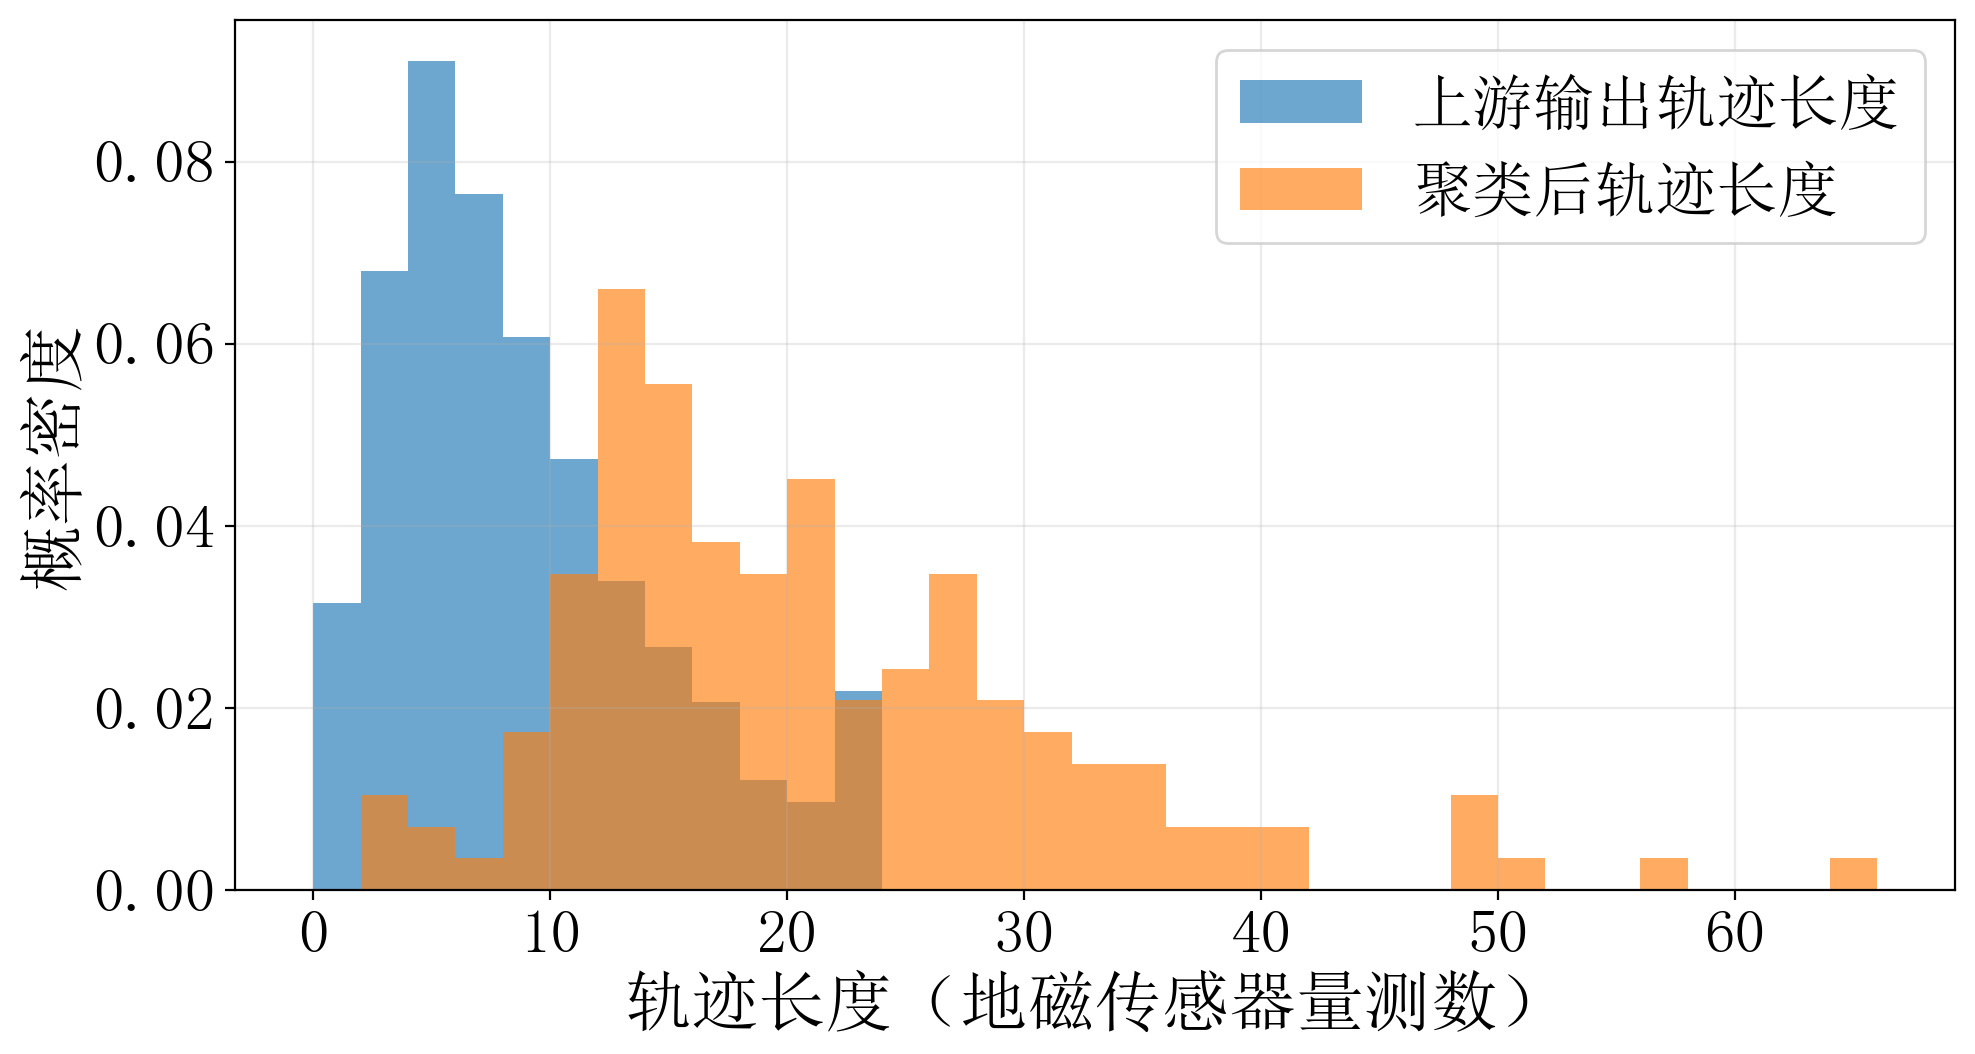
\includegraphics[width=0.78\textwidth]{4_3_length_distribution_v2.png}
	\caption{重构前后轨迹长度分布对比图}
	\label{fig:4_3_length_distribution}
\end{figure}

\subsection{整体重构效果对比分析}

为更系统地评价方法性能，下面给出不同方法在主场景下的对比结果。所有方法均采用同一批上游输出样本作为输入，并保持一致的样本到达顺序，不引入额外人工后处理。由于仅保留上游输出不会产生新的跨缺测片段拼接关系，因此表~\ref{tab:4_2_overall_metrics} 主要比较三种实际执行重构的方法。CEDAS 基线采用在线密度聚类思路，CluStream 基线采用微簇摘要机制，二者都属于通用流式聚类方法；本文方法则进一步引入了面向轨迹片段接续的时间顺序约束、方向约束、地磁辅助判别和簇尾摘要更新机制。主场景中，重构前的初始碎片数均为 $178$。

\begin{table}[htbp]
	\centering
	\caption{不同方法在主场景下的总体聚类重构效果对比}
	\label{tab:4_2_overall_metrics}
	\renewcommand{\arraystretch}{1.15}
	\resizebox{\textwidth}{!}{
		\begin{tabular}{lcccccc}
			\toprule
			方法 & $P_{\mathrm{link}}$ & $R_{\mathrm{link}}$ & $F1_{\mathrm{link}}$ & $R_{\mathrm{wm}}$ & $\mathrm{Frag}_{\mathrm{drop}}$ & $\mathrm{FMI}$ \\
			\midrule
			CEDAS 基线      & 0.5217 & 0.1086 & 0.1798 & 0.4783 & 26  & 0.2380 \\
			CluStream 基线  & 0.6014 & 0.3756 & 0.4624 & 0.3986 & 91  & 0.4753 \\
			本文方法        & 0.9208 & 0.8416 & 0.8794 & 0.0792 & 104 & 0.8803 \\
			\bottomrule
	\end{tabular}}
\end{table}

由表~\ref{tab:4_2_overall_metrics} 可以看出，两种通用在线聚类方法都能够在一定程度上减少碎片数，但对本章任务的适配程度明显不同。CEDAS 基线的召回率较低，而错并率接近一半，说明它虽然能够完成部分合并，却很难准确区分哪些样本应当接到同一条轨迹中。CluStream 基线的结果明显好于 CEDAS，说明簇摘要机制对片段流组织是有帮助的，但其 $R_{\mathrm{wm}}$ 仍然较高，$\mathrm{FMI}$ 也偏低，表明仅依靠通用特征距离仍容易在时空位置相近的样本之间产生混淆。

相比之下，本文方法在各项核心指标上均取得了最优结果。其 $F1_{\mathrm{link}}$ 达到 $0.8794$，明显高于 CluStream 基线的 $0.4624$ 和 CEDAS 基线的 $0.1798$；错并率 $R_{\mathrm{wm}}$ 降至 $0.0792$，远低于两类基线方法；碎片消减量 $\mathrm{Frag}_{\mathrm{drop}}$ 达到 $104$，同时全局一致性指标 $\mathrm{FMI}$ 提升至 $0.8803$。这一结果说明，本文方法的优势不仅在于能够合并更多断裂样本，更在于合并后的轨迹边界更准确、整体分组也更接近真实车辆轨迹。结合前面的可视化结果和长度分布变化可以看出，所提方法能够在控制误并风险的同时有效缓解长时缺测造成的碎片化问题。

\subsection{不同漏检强度下的重构性能对比分析}

为考察长缺测强度变化对重构性能的影响，本文在与上游算法一致的仿真道路场景、车流生成参数和地磁响应设置下生成量测序列，并在单点量测层面注入不同强度的漏检扰动。随后，由上游算法输出轨迹片段及未完成关联的单点量测，再将这些样本作为本章重构算法的输入。这样得到的结果能够直接反映完整处理链路在不同缺测强度下的表现。

\begin{figure}[htbp]
	\centering
	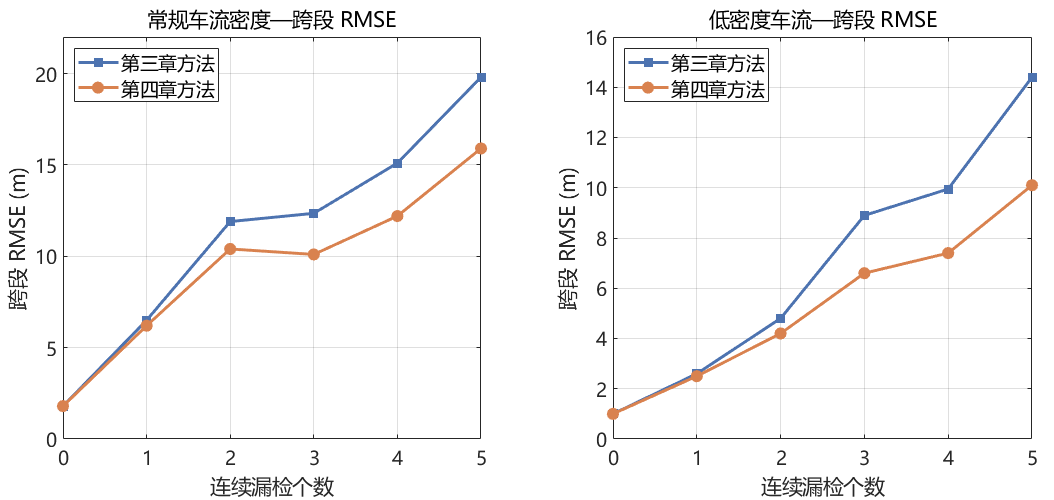
\includegraphics[width=0.93\textwidth]{code/chapter4/experiment123/chapter4_results/exp1/4_7_duiibi_v2.png}
	\caption{上游算法与加入片段级聚类重构后的跨段 RMSE 对比图}
	\label{fig:ch4_rmse_upstream_cluster}
\end{figure}

图~\ref{fig:ch4_rmse_upstream_cluster} 先比较了仅采用上游算法与在其后接入片段级重构两种处理链路的跨段 RMSE。可以看到，当连续缺测长度较小时，两种方法在不同车流密度下的差别并不明显，这说明上游算法对短时漏检本身已经具有较好的处理能力，而片段级重构不会对其原有结果造成明显扰动。随着连续缺测长度继续增加，后续重构带来的收益开始变得明显。在常规车流密度下，当连续漏检个数达到 $5$ 时，仅采用上游算法的跨段 RMSE 上升到 $19.80\,\mathrm{m}$，加入片段级重构后下降到 $13.80\,\mathrm{m}$；在低密度车流条件下，对应误差由 $14.40\,\mathrm{m}$ 下降到 $10.10\,\mathrm{m}$。这说明片段级重构的主要作用不是替代上游算法对短间断的处理能力，而是在上游输出已经碎片化之后，继续利用样本之间的时间、方向和地磁一致性恢复更长缺测区间中的断裂关系。

\begin{figure}[htbp]
	\centering
	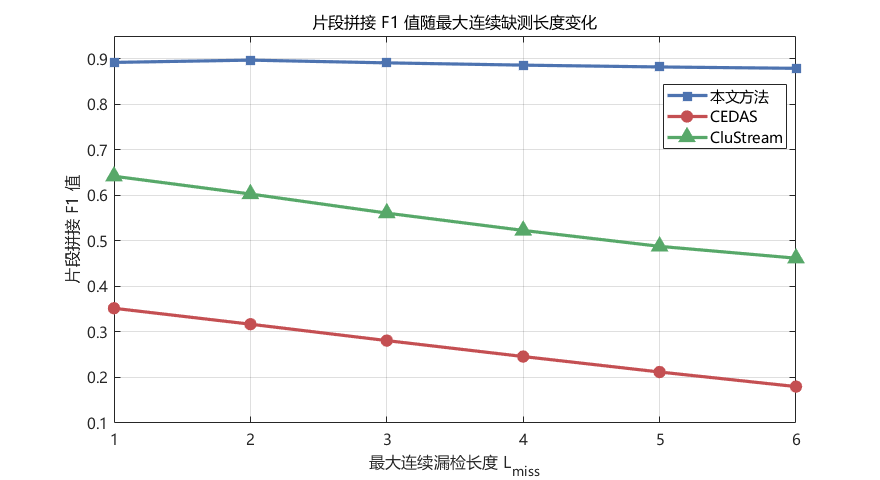
\includegraphics[width=0.85\textwidth]{code/chapter4/experiment123/chapter4_results/exp1/4_5_lianxvquece.png}
	\caption{片段拼接 $F1$ 值随最大连续缺测长度变化结果图}
	\label{fig:ch4_f1_vs_lmiss}
\end{figure}

\begin{figure}[htbp]
	\centering
	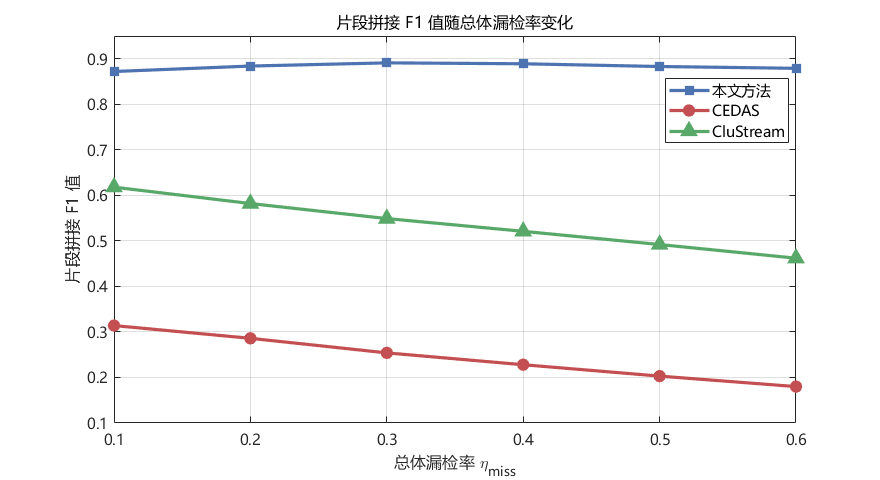
\includegraphics[width=0.85\textwidth]{code/chapter4/experiment123/chapter4_results/exp1/4_6_loujianlv.png}
	\caption{片段拼接 $F1$ 值随总体漏检率变化结果图}
	\label{fig:ch4_f1_vs_missrate}
\end{figure}

图~\ref{fig:ch4_f1_vs_lmiss} 和图~\ref{fig:ch4_f1_vs_missrate} 进一步给出了不同方法在不同缺测强度下的片段拼接 $F1$ 值变化情况。三种方法的性能排序始终保持一致，均为本文方法最好，CluStream 次之，CEDAS 最低。随着最大连续缺测长度 $L_{\mathrm{miss}}$ 增大或总体漏检率 $\eta_{\mathrm{miss}}$ 升高，三种方法的性能都会下降，但本文方法的曲线始终更高，也更平稳。以最大连续缺测长度为例，当 $L_{\mathrm{miss}}=6$ 时，本文方法的 $F1_{\mathrm{link}}$ 仍保持在 $0.880$ 左右，而 CluStream 和 CEDAS 分别下降到 $0.462$ 和 $0.181$。以总体漏检率为例，当 $\eta_{\mathrm{miss}}=0.6$ 时，本文方法的 $F1_{\mathrm{link}}$ 仍约为 $0.880$，而 CluStream 和 CEDAS 分别仅为 $0.462$ 和 $0.182$。这说明通用在线聚类方法虽然能够处理一般样本流，但在缺测增强、候选关系更复杂时，容易因为缺少轨迹接续约束而出现明显退化；本文方法则由于显式利用了簇尾方向、时间顺序和地磁代表值，在较强缺测条件下仍能保持较好的样本拼接能力。结合图~\ref{fig:ch4_rmse_upstream_cluster} 可以看出，在上游算法之后增加片段级重构，能够把系统对连续缺测的有效恢复范围进一步向更困难的场景延伸。

\FloatBarrier



\section{本章小结}

本章针对系统长期运行后因传感器老化、检测能力下降以及复杂交通工况共同作用而引发的长缺测轨迹碎片化问题，在第三章上游在线跟踪结果基础上，提出了一种面向长缺测工况的片段级在线聚类与轨迹重构方法。与前一章主要围绕单点量测级在线跟踪展开不同，本章不再继续展开状态递推，而是将上游输出的轨迹片段及未得到关联的单点量测统一表示为聚类样本，并据此构建簇图结构与簇尾摘要。算法具体而言，首先将片段压缩表示为方向向量、地磁代表值、支持度和起止时间戳，以尽可能少的变量保留轨迹重构所需的关键信息；随后，围绕簇初始化、融合方向约束的聚类相似度评分、簇尾摘要更新以及生命周期管理等关键环节，建立了完整的在线聚类与轨迹重构流程。由此，长缺测后的轨迹恢复被统一表述为一个面向片段流的在线增量归并过程。实验结果表明，所提方法能够有效恢复长缺测后断裂的车辆轨迹，降低错误拼接和身份切换，并在中等至较高缺测强度范围内保持较稳定的片段拼接性能。综合来看，基于簇图结构与聚类相似度评分的片段级在线聚类方法，为多地磁传感器系统在长期运行条件下的轨迹重构提供了清晰且可实现的技术路径。


\chapter{总结与展望}

\section{总结}

随着高速公路运行监测和精细化管理需求不断提高，如何利用布设在道路上的地磁传感器稳定获取车辆连续轨迹，已成为智能交通系统中的重要问题。地磁传感器具有成本较低、布设灵活、受光照和天气影响较小等特点，适合在道路场景中长期部署。地磁传感器虽然能够持续感知车辆通过引起的局部磁场变化，但仅依靠离散检测结果难以直接形成完整轨迹，还需要进一步解决量测乱序、漏检、多检、邻道干扰、双车并行混淆以及长时缺测后的轨迹碎片化等问题。针对上述问题，本文围绕单向双车道高速公路场景下的多地磁传感器车辆目标跟踪开展研究，构建了由在线跟踪和轨迹片段重构组成的完整处理流程，为多地磁传感器条件下的车辆连续跟踪提供了方法支撑。

本文主要工作如下：

（1）本文对现有的地磁传感器车辆检测和目标跟踪技术和在线聚类等相关研究进行了梳理和综述，分析了多地磁传感器用于车辆目标跟踪的研究意义。在此基础上，结合单向双车道高速公路场景，建立了多地磁传感器系统架构，并对其部署模型和量测模型进行介绍，为后续算法设计提供统一的问题描述和理论基础。

（2）针对非理想量测条件下的车辆目标跟踪问题，本文提出了面向多地磁传感器数据的在线跟踪方法。该方法围绕量测时序矫正、车辆运动状态估计、数据关联和轨迹管理展开设计，通过时间窗口缓存和固定滞后处理改善量测乱序带来的影响，并通过地磁传感器检测可靠性建模与自适应更新、邻道干扰与双车并行场景递推判别以及车道状态更新与修正，提高了复杂条件下量测归属和轨迹维持的稳定性。仿真与实测结果表明，所提方法能够较好地保持车辆轨迹连续性，并在多种非理想条件下表现出较好的适应能力。

（3）针对长时缺测条件下的轨迹碎片化问题，本文进一步提出了基于在线聚类的轨迹片段重构方法。该方法将上游输出的轨迹片段和未完成关联的单点量测统一表示为聚类样本，构建簇图结构与簇尾摘要，并围绕簇初始化、融合方向与地磁辅助的聚类相似度计算、簇更新与生命周期管理等关键环节完成断裂轨迹片段的在线归并与重构。实验结果表明，所提方法能够有效恢复长时缺测后的断裂轨迹，减少错误拼接和身份混淆，进一步提升最终输出轨迹的完整性和一致性。

总体来看，本文围绕多地磁传感器车辆目标跟踪这一问题，形成了从前端量测处理、在线跟踪到后续轨迹片段重构的完整技术路线。相关研究不仅丰富了地磁传感器在车辆目标跟踪方向上的应用方法，也为高速公路运行监测和车辆轨迹级交通分析提供了可行的技术支撑。

\section{未来展望}

尽管本文围绕单向双车道高速公路场景下的多地磁传感器车辆目标跟踪问题开展了较为系统的研究，并取得了较好的效果，但距离更加复杂的实际应用仍有进一步提升空间。后续可从以下几个方面继续展开研究。

（1）本文的方法建立在单向双车道场景和较规则车辆运动过程基础上，对于当前方法是否适用于多车道场景、匝道汇入汇出区域、及更复杂道路结构场景还未知，还需要进一步研究更加一般化的场景建模、车道状态表达和轨迹管理方法，以提升算法在复杂道路环境中的适用范围。

（2）当前方法已经对地磁传感器检测可靠性进行了在线自适应处理，但部分参数设置仍具有一定经验性，对地磁信息的利用也主要集中在地磁峰值和地磁代表值等较低维特征上。后续可进一步研究参数自整定方法，并挖掘更加丰富的地磁波形特征和时序特征，以提高对相邻车辆和相似轨迹片段的区分能力。

（3）本文分别针对单点量测在线跟踪和长时缺测后的轨迹片段重构进行了设计，两部分之间已经形成了较好的前后衔接关系，但仍有进一步联合优化的空间。后续可研究更紧密的协同处理方法，使轨迹片段重构结果能够更早参与轨迹管理和状态修正，从而进一步提升整条处理链路的一致性和恢复能力。

（4）从工程应用角度看，后续还需要在更长时间跨度、更大部署范围和更多交通状态条件下开展持续验证，并进一步优化算法的计算开销和存储开销，增强系统在长期运行条件下的稳定处理能力和实时处理能力，为多地磁传感器车辆目标跟踪在实际高速公路中的推广应用提供支撑。
\end{document}